\documentclass[defaultstyle,10pt,master,Arial]{ISTthesisEN}
% Use ISTthesisPT for portuguese version 

\typeout{}
\typeout{--------------------------------------------------------------}
\typeout{ +---+ Thesis Template                            }
\typeout{ +---+      Version 1.7.8, April 2016                         }
\typeout{ +---+  for Instituto Superior Tecnico (IST),                 }
\typeout{ +---+  Universidade Técnica de Lisboa                         }
\typeout{ * Using Thesis Style from Pedro Tomás                                }
\typeout{ * Created to write Dissertations                             }
\typeout{ * Conforms with IST Master Degree format and with most important packages setup        }
\typeout{ * Should conform with IST PhD Degree format (not verified)   }
\typeout{                                                              }
\typeout{ AUTHOR: Miguel Amador and João Marques                                          }
\typeout{                                                              }
\typeout{Important: Use all files in the archive, since this is based in all them. Modify dummy files at wish.                                                              }
\typeout{--------------------------------------------------------------}
\typeout{}

% MY OWN PACKAGES
\usepackage{cuted}
\usepackage{bm}
\usepackage{bbm}
\usepackage{setspace}
\pagenumbering{arabic}
\usepackage{scrextend}
\usepackage{ragged2e}
\usepackage{xcolor}
\usepackage{dirtytalk}
\usepackage{setspace}
\newcommand*\chem[1]{\ensuremath{\mathrm{#1}}}
\def\Pm{\mathrel{\raise -1.2pt \hbox{\tiny(}\! 
                 \raise 1.5pt \hbox{+}
                 \settowidth {\dimen03} {+}
                 \hskip-\dimen03
                 \raise -2.6pt \hbox {$-$}
                 \!\raise -1.2pt \hbox{\tiny)}}}
\usepackage{simplewick}
\newcommand{\angstrom}{\textup{\AA}}
% Defines an additional alphabet... not required in most cases
% ------------------------------------------------------------
% \DeclareMathAlphabet{\mathpzc}{OT1}{pzc}{m}{it}

% PACKAGE babel:
% ---------------
% The 'babel' package may correct some hyphenisation issues of latex. 
% However in most situations it is not required.
\usepackage[portuguese,english]{babel}


% PACKAGE fontenc:
% -----------------
% chooses T1-fonts and allows correct automatic hyphenation.
%\usepackage[T1]{fontenc}
%\usepackage[latin1]{inputenc}
\usepackage[utf8]{inputenc}
\usepackage[T1]{fontenc}
%\usepackage{lmodern} %will change font type

% Package ulem.
\usepackage{ulem} % Allows the use of other text emphatizer commands
\normalem %defines \emph{} to italic, instead of underline. 
\raggedbottom %declaration makes all pages the height of the text on that page. No extra vertical space is added. The \flushbottom declaration makes all text pages the same height, adding extra vertical space when necessary to fill out the page.

% PACKAGE date time:
% -----------------
% Lets you alter the format of the date that \today returns.
\usepackage{datetime}
\newdateformat{todaythesis}{%
\monthname[\THEMONTH]  \THEYEAR}

% PACKAGE latexsym:
% -----------------
% Defines additional latex symbols. May be required for thesis with many math symbols.
\usepackage{latexsym}

% PACKAGE amsmath, amsthm, amssymb, amsfonts:
% -------------------------------------------
% This package is typically required. Among many other things it adds the possibility
% to put symbols in bold by using \boldsymbol (not \mathbf); defines additional 
% fonts and symbols; adds the \eqref command for citing equations. I prefer the style
% "(x.xx)" for referering to an equation than to use "equation x.xx".
\usepackage{amsmath, amsthm, amssymb, amsfonts, amsbsy}
\DeclareMathOperator{\Tr}{Tr}
%\DeclareMathOperator{\det}{det}

% PACKAGE multirow, colortbl, longtable:
% ---------------------------------------
% These packages are most usefull for advanced tables. The first allows to join rows 
% throuhg the command \multirow which works similarly with the command \multicolumn
% The second package allows to color the table (both foreground and background)
% The third package is only required when tables extend beyond the length of one page;
% with compatibilities with the tabular environment. The last allow the definitions of landscape pages, allowing the use of a different orientation for wider graphics or tables. See package documentation to see the implementation.
\usepackage{multirow}
\usepackage{colortbl}
\usepackage{supertabular}
\usepackage{pdflscape}
% \usepackage{longtable}

% PACKAGE graphics, epsfig, subfigure, caption:
% ---------------------------------------------
% Packages for figures... well you will certainly need these packages, with the exception
% of the 'caption' package. This only allows to define extra caption options.
% Notice that subfigure allows to place figures within figures with its own caption. It
% should be avoided to create an eps file with subfigures. That will mean that you won't be 
% able to reference those subfigures. Instead create an EPS file (the only graphics format supported
% by latex) for each of the subfigures and then use the command \subfigure (see below).
\usepackage{graphics}
\usepackage{graphicx}
\usepackage{epsfig}
\usepackage[hang,small,bf]{subfigure}
%\usepackage[footnotesize,bf,center]{caption}
\usepackage{dcolumn}
\usepackage{bm}
\usepackage{booktabs}
\usepackage{rotating}
\usepackage{multirow}

\usepackage[font=small,labelfont=bf,textfont=normalfont]{caption}

% PACKAGE algorithmic, algorithm
% ------------------------------
% These packages are required if you need to describe an algorithm.
 \usepackage{algorithmic}
 \usepackage[chapter]{algorithm}
 
\usepackage[backend=biber,style=nature,sorting=none]{biblatex}
%\addbibresource{/Users/franciscobrito/Dropbox/Mendeley/MScThesis/MScThesis.bib}
\addbibresource{references.bib}

% PACKAGE acronyum
% -----------------
% This package is most useful for acronyms. The package guarantees that all acronyms definitions are 
% given at the first usage. IMPORTANT: do not use acronyms in titles/captions; otherwise the definition 
% will appear on the table of contents.
\usepackage[printonlyused]{acronym}
\usepackage[titletoc,title,header]{appendix}
\usepackage[noauto]{chappg}
%The following line assures that each chapter deals with acronyms idependently.
%You may also do it manually by calling acresetall anywhere in the documento to reset the acronyms behaviour. 
\preto\chapter\acresetall

% PACKAGE extra_functions
% -----------------
% My Personal package: defines the following commands:
% \fancychapter{chaptername) -> Prints a fancier chapter (you can also use the fancychapter package for this)
% \hline{width} -> use for a replacement of the \hline command
% \Mark1, \Mark2, \Mark3, ...
\usepackage{extra_functions}


% PACKAGE hyperref
% -----------------
% Set links for references and citations in document
\usepackage[plainpages=false]{hyperref}
\hypersetup{
             colorlinks=false,
             citecolor=red,
             breaklinks=true,
             bookmarksnumbered=true,
             bookmarksopen=true,
             pdftitle={Development of a QMC code to tackle interacting electronic systems in 2D with application to TMD nanoribbons},
             pdfauthor={Francisco Brito},
             pdfsubject={Master Thesis in Physics Engineering},
             pdfcreator={Francisco M. O. Brito},}
\usepackage{float}
\usepackage{url}
%\usepackage[final]{listofsymbols}
\usepackage{symlist}

% Set paragraph counter to alphanumeric mode
\renewcommand{\theparagraph}{\Alph{paragraph}~--}

\newcommand{\figref}[1]{Figure \ref{#1}}
\newcommand{\equationref}[1]{Equation (\ref{#1})}
\newcommand{\tableref}[1]{Table (\ref{#1})}

\newcommand{\textreg}{$\textsuperscript{\textregistered}$}

\definecolor{silver}{rgb}{0.6, 0.6, 0.6}

\newcommand\rddots 
   {\mathinner{\mkern1mu 
       \raise 1pt\hbox{.}\mkern2mu 
       \raise 4pt\hbox{.}\mkern2mu 
       \raise 7pt\hbox{.}\mkern1mu}} 

\hoffset 0in
\voffset 0in

%Alternative set of page geometry
%\oddsidemargin 0.71cm
%\evensidemargin 0.04cm
%\marginparsep 0in
%\topmargin -0.25cm
%\textwidth 15cm
%\textheight 23.5cm

\usepackage[top=2.5cm, bottom=2.5cm, inner=2.9cm, outer=2.5cm]{geometry}

\usepackage{fancyhdr}
\pagestyle{fancy}
\renewcommand{\chaptermark}[1]{\markboth{\thechapter.\ #1}{}}
\renewcommand{\sectionmark}[1]{\markright{\thesection\ #1}}
\fancyhf{} 
%\fancyhead[LE]{\bfseries\nouppercase{\leftmark}}
%\fancyhead[RO]{\bfseries\nouppercase{\rightmark}}
\fancyfoot[LE,RO]{\bfseries\small\thepage}
\renewcommand{\headrulewidth}{0.0pt}
\renewcommand{\footrulewidth}{0.0pt}
\addtolength{\headheight}{2pt} % make space for the rule
\fancypagestyle{plain}{% Used in Chapter titles
   \fancyhead{} % get rid of headers
   \renewcommand{\headrulewidth}{0pt} % and the line
   \renewcommand{\footrulewidth}{0pt}
   \fancyfoot[LE,RO]{\bfseries\small\thepage}
}

\fancypagestyle{begin}{%
   \fancyhead{}
   \renewcommand{\headrulewidth}{0pt}
   \renewcommand{\footrulewidth}{0pt}
   \fancyfoot[LE,RO]{\bfseries\small\thepage}
}
\fancypagestyle{document}{%
	\fancyhf{} 
	\fancyhead[LE]{\bfseries\nouppercase{\leftmark}}
	\fancyhead[RO]{\bfseries\nouppercase{\rightmark}}
	\fancyfoot[LE,RO]{\bfseries\small\thepage}
	%\renewcommand{\headrulewidth}{0pt}
	%\renewcommand{\footrulewidth}{0pt}
	\addtolength{\headheight}{2pt} % make space for the rule
}
\fancypagestyle{documentsimple}{%
	\fancyhf{}
	\fancyfoot[LE,RO]{\bfseries\small\thepage}
	%\renewcommand{\headrulewidth}{0pt}
	%\renewcommand{\footrulewidth}{0pt}
	\addtolength{\headheight}{2pt} % make space for the rule
}
\setcounter{secnumdepth} {5}
\setcounter{tocdepth} {5}
\renewcommand{\thesubsubsection}{\thesubsection.\Alph{subsubsection}}

\renewcommand{\subfigtopskip}{0.3 cm}
\renewcommand{\subfigbottomskip}{0.2 cm}
\renewcommand{\subfigcapskip}{0.3 cm}
\renewcommand{\subfigcapmargin}{0.2 cm}

\graphicspath{{Figures/}}


\begin{document}

\onehalfspacing
\selectlanguage{english}

\pagestyle{begin}
\setcounter{page}{1} \pagenumbering{Alph}

% Add PDF bookmark 
\pdfbookmark[0]{Title}{Title}

\thispagestyle{empty}

\begin{flushleft} ~\\ \vspace{-12mm} \hspace{-12mm}

\includegraphics[width=50mm]{Cover/istnewlogo}
\vspace{10mm}
%~\\ \vspace{50mm} % gráficos
\\ \begin{center} 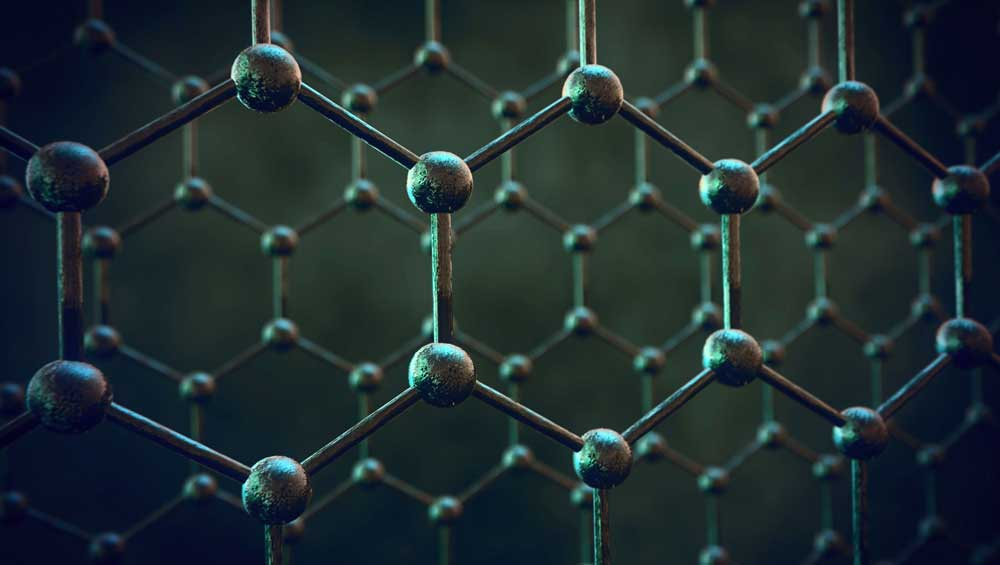
\includegraphics[height=50mm]{Cover/coverimage}  \end{center} % gráficos
 \vspace{5mm}
\centering
\LARGE \textbf{Development of a QMC code to tackle interacting electronic systems in 2D with application to TMD nanoribbons}
\\
\vspace{15mm}
\Large \textbf{Francisco Monteiro de Oliveira Brito} \\
\vspace{12mm}
\large Thesis to obtain the Master of Science Degree in
\\ \vspace{2mm}
\LARGE \textbf{Physics Engineering}
\\ \vspace{10mm}
\large Supervisor(s): Prof. Eduardo Filipe Vieira de Castro  \\
\large Prof. João Manuel Viana Parente Lopes 
\\ \vspace{10mm}
\Large \textbf{Examination Committee}
\\ \vspace{5mm}
\large Chairperson: Prof. Lorem \\
\large Supervisor: Prof. Eduardo Filipe Vieira de Castro \\
\large Co-Supervisor: Prof. João Manuel Viana Parente Lopes  \\
\large Members of the Committee: Dr. Lorem Ipsum \\
%\vspace{15mm}
\vspace{5mm}
\Large \textbf{\todaythesis\today} \\
\let\thepage\relax
\end{flushleft}
\pagebreak


\clearpage
% Since I am using double sided pages, the second page should be white.
% Remember that when delivering the dissertation, IST requires for the cover to appear twice.

\thispagestyle{empty}
\cleardoublepage

\setcounter{page}{1} \pagenumbering{roman}

\baselineskip 18pt % line spacing: -12pt for single spacing
                   %               -18pt for 1 1/2 spacing
                   %               -24pt for double spacingnts}
 
\thispagestyle{empty}
\hbox{} \vfill
\begin{flushright}
\small \textit{\textbf{The behavior of large and complex aggregates of elementary particles, it turns out, is not to be understood in terms of a simple extrapolation of the properties of a few particles.}}
\\ \vspace{2mm}  
\scriptsize P. W. Anderson
\end{flushright}

\clearpage
\thispagestyle{empty}
\cleardoublepage

\pdfbookmark{Acknowledgments}{Acknowledgments}
\begin{acknowledgments} 

I want to start by thanking my parents Laura and João, and the rest of my family, biological, and non-biological.
They did everything they could (and more) to ensure that I had the opportunities that led me to develop this work.
They taught me to do things out of love, and that is a lesson I carry with me everyday of my life.

Then, I want to thank Beatriz for supporting me unconditionally in everything I do, for always being  so kind and sincere, for brightening up my life and making me smile so much, and for the great love and understanding she shows everyday.
Quoting Carl Sagan, \say{In the vastness of space and the immensity of time, it is my joy to share a planet and an epoch} with her.

Of course, I would also like to thank my supervisors Prof. Eduardo Filipe Vieira de Castro, and Prof. João Manuel Viana Parente Lopes for the openness, support, and tireless will to teach me, and learn with me.
Not only did they provide valuable scientific insight, but they also showed great humaneness in guiding me through the journey I embarked on during the last year.

I also want to express the gratitude and admiration I feel for my colleagues at Centro de Física do Porto, the Theoretical Physics Center at University of Porto.
They worked beside me almost daily, discussing and criticizing my work, providing great help, be it by cheering me up in darker times, or by celebrating even the tiniest achievements in my work.

I am grateful for having had great teachers, who inspired me to seek knowledge over the years. I wish to thank all of them. In particular, I want to mention Maria da Luz and Vítor Santos who got me excited about Physics in the first place, and Profs. Joaquim Agostinho Gomes Moreira and João M. B. Lopes dos Santos for sparking my enthusiasm for condensed matter physics. Moreover, I would like to thank Dr. Miklós Lajkó, Dr. Jon Demidio for what they taught me during my stay in Lausanne, and Prof. Frédéric Mila for introducing me to the many currents topics of research in condensed matter theory, and sharing valuable insight.

Lastly, I want to thank a number of close friends who constantly support me, of which I will mention a few: Mateus, Carol, Marta, Bárbara, Andreia, Inês Lopes, Inês Viegas, Nuno, Glênio, Angélica, Raquel, Tiago, Miguel, Branca, Pedro, and Isabela. 

\end{acknowledgments}
\clearpage
\thispagestyle{empty}
\cleardoublepage
\selectlanguage{english}
\begin{abstract}

Cooperative behavior has been at the forefront of condensed matter physics research for the most part of the last half-century.
This complex systems era has brought about a concept called emergence, which is now overarching.
In particular, in strongly correlated electron systems, emergent phenomena lead to a variety of exotic properties that defy intuition.

The discovery of two-dimensional materials, has renewed interest in the many-electron problem since electron-electron interactions  play an important role in the description of many of the properties of these systems.
Moreover, the rapid increase in computational power, and algorithmic sophistication has made it possible to attack many problems in the field that were previously intractable.
In this work, we focus on a particular class of two-dimensional materials showing a wealth of fascinating electronic and optical properties: Transition Metal Dichalcogenides.

We investigate emerging edge-state magnetism in a type of nanostructure called a nanoribbon, so called because it resembles a ribbon, being much longer on direction than on the other.
To study this phenomenon, we consider a recently introduced symmetry-based tight-binding model that is found to capture most properties related to the edge physics of the problem.
Then, we generalize it to interacting case by considering intra-orbital Hubbard-type interactions.

Our approach to this problem is two-fold.
We start by performing original numerical mean field calculations and build an approximate physical picture of the system at hand.
Then, we use our own implementation of the unbiased, state-of-the-art Determinant Quantum Monte Carlo algorithm to simulate this interacting, quantum many-fermion system.

\end{abstract}
\begin{keywords}
\acs{2D} Materials, Hubbard Model, Strongly Correlated Electrons, \acl{TMD} Nanoribbons, Mean Field Theory, Determinant / Auxiliary Field \acf{QMC} (English)
\end{keywords}
\clearpage
\thispagestyle{empty}
\cleardoublepage
\selectlanguage{portuguese}
\begin{resumo}

O objectivo deste trabalho ... (Português)

\end{resumo}
\begin{palavraschave}
Materiais Bidimensionais, Modelo de Hubbard, Eletrões Fortemente Correlacionados, Nanofitas de Dicalcogenetos de Metais de Transição, Teoria de Campo Médio, Monte Carlo Quântico: Método do Determinante ou Campo Auxiliar (Português)
\end{palavraschave}
\clearpage
\thispagestyle{empty}
\cleardoublepage
\selectlanguage{english}
% This is required for the fancy chapters
\dominitoc
\dominilof
\dominilot

%%%%%%%%%%%%%%%%%%%%%%%%%%%%%%%%%%%%%%%%%%%%%%%%%%%%%%%%%%%%%%%%%%%%%%
% List of contents
%\renewcommand{\baselinestretch}{1}
\pdfbookmark[0]{Index}{index}
\pdfbookmark[1]{Contents}{toc}
\tableofcontents
% \contentsline{chapter}{References}{\pageref{bib}}
\clearpage
\thispagestyle{empty}
\cleardoublepage
%\renewcommand{\baselinestretch}{1.5}
%%%%%%%%%%%%%%%%%%%%%%%%%%%%%%%%%%%%%%%%%%%%%%%%%%%%%%%%%%%%%%%%%%%%%%
% List of figures
\pdfbookmark[1]{List of Figures}{lof}
\listoffigures
\clearpage
\thispagestyle{empty}
\cleardoublepage

%%%%%%%%%%%%%%%%%%%%%%%%%%%%%%%%%%%%%%%%%%%%%%%%%%%%%%%%%%%%%%%%%%%%%%
% List of tables
\pdfbookmark[1]{List of Tables}{lot}
\listoftables
\clearpage
\thispagestyle{empty}
\cleardoublepage

% %%%%%%%%%%%%%%%%%%%%%%%%%%%%%%%%%%%%%%%%%%%%%%%%%%%%%%%%%%%%%%%%%%%%%%
% % List of algorithms
% Requires packages algorithmic, algorithm
% \pdfbookmark[1]{List of Algorithms}{loa}
% \listofalgorithms
% \cleardoublepage
\acresetall
% Remember that in the list of tables titles are set manually
% %%%%%%%%%%%%%%%%%%%%%%%%%%%%%%%%%%%%%%%%%%%%%%%%%%%%%%%%%%%%%%%%%%%%%%
 % List of acronyms
\pdfbookmark[1]{List of Acronyms}{loac}

\chapter*{Abbreviations}


% See more at http://staff.science.uva.nl/~polko/HOWTO/LATEX/acronym.html

\begin{acronym}
%\acro{acro}{Dummy Acronym}
\acro{QMC}{Quantum Monte Carlo}
\acro{TMD}{Transition Metal Dichalcogenide}
\acro{LG}{Landau Ginzburg}
\acro{2D}{two-dimensional}
\acro{PBC}{periodic boundary condition}
\acro{OBC}{open boundary condition}
\acro{PHS}{Particle-hole symmetry}
\acro{AF}{antiferromagnetic}
\acro{PHT}{Particle-hole transformation}
\end{acronym}


%\ac{acro} 
% The first time you use this, the acronym will be written in full with the acronym in parentheses: supernova (SN). At later times it will just print the acronym: SN.

%\acf{acro}
% written out form with acronym in parentheses, irrespective of previous use

%\acs{acro}
% acronym form, irrespective of previous use

%\acl{acro}
% written out form without following acronym

%\acp{acro}
% plural form of acronym by adding an s. \acfp. \acsp, \aclp work as well.

\clearpage
\thispagestyle{empty}
\cleardoublepage




%%%%%%%%%%%%%%%%%%%%%%%%%%%%%%%%%%%%%%%%%%%%%%%%%%%%%%%%%%%%%%%%%%%%%%
% List of symbols
\pdfbookmark[1]{List of Symbols}{los}

\listofsymbols

\clearpage
\thispagestyle{empty}

\cleardoublepage
% Pages number is starting now with arabic style... until now it was on roman mode
\pagenumbering{arabic} \setcounter{page}{1}
\baselineskip 18pt
\selectlanguage{english}
% Define the title of Chapter Table of Contents
\mtcsettitle{minitoc}{Contents}
\pagestyle{documentsimple}%Simple head
% Insert chapters here

\fancychapter{Introduction}
\label{cap:int}

\slshape

The isolation of graphene in 2004 has led to a growing interest of the scientific community in \ac{2D} materials revealing extraordinary properties.
Among them are \acp{TMD}, appearing in the form of a variety of nanostructures.
Unlike in graphene, where electron interactions are relatively weak, in \acp{TMD}, electrons are strongly correlated, and one cannot overlook the interactions between them.
Analytical approaches to the solution of the problem are either hopeless, or rely on possibly unrealistic approximations.
In fact, the increased complexity of the models describing such highly correlated  materials, compared to their graphene counterparts, calls for sophisticated computer simulation methods, most notably \ac{QMC}.
In this introductory chapter, we start by  reviewing the literature on the physics of \acp{TMD}, focusing on their basic properties.
Then, we present a survey of simulation methods belonging to the \acl{QMC} class.
We introduce some basic concepts, and motivate the choice of the particular used  method.
Finally, we summarize our original contributions, and outline the structure of the thesis.

\normalfont

\section{Motivation}
\label{sec:motivation}

It might seem surprising that \ac{2D} systems were not considered as a real possibility before the discovery of graphene since they are often idealized in thought experiments, for example when investigating toy models of more complex higher dimensional systems.
In fact, while thin film deposition on comparably thicker substrates was commonplace long before 2004, \ac{2D} layers were thought not to exist independently from their 3D base.
Their existence was not expected \emph{a priori} because at first sight they seem to violate the Mermin-Wagner-Hohenberg theorem \cite{mermin_absence_1966, coleman_there_1973, hohenberg_existence_1967}, a no-go theorem that forbids ordering below three dimensions at finite temperature\footnote{\ac{2D} materials can be stable because not all the conditions of Mermin-Wagner-Hohenberg theorem are verified, namely the condition of short-ranged interactions. In the particular case of graphene sheets, ripples appear, which implies that the material is not strictly \ac{2D}, and thus can be stabilized. The issue is subtle, and is beyond the scope of this work.}.
The discovery of graphene paved the way for the search for similarly stable \ac{2D} materials, and since it was isolated, a plethora of these has been discovered.
A vast set of open problems remains to be solved within the realm of the fascinating and counterintuitive properties of the now huge variety of existing \ac{2D} systems.
In particular, in some of these, the effect of electron interactions is non negligible, leading to emergent phenomena.
These are collective effects that emerge as a result of the interactions between the individual components of a system.
The properties of the system's components do not directly percolate up; instead, they shape the interactions that dictate the system's properties sometimes in rather unexpected ways, leading to unusual behavior.

Interacting electron systems are often tackled by carrying out computer simulations.
\ac{QMC} is a family of numerical methods that are  amply applicable to condensed matter physics problems, and that are particularly well suited to study strongly correlated electrons.
Despite the system size being constrained due to limited simulation time, reliable, accurate and unbiased solutions are provided to the otherwise intractable quantum many-body problem.
The class of \acs{QMC} algorithms that is used in this work was introduced in the 1980's in a series of seminal papers by Hirsch and \acl{BSS}\footnote{After whom the \ac{BSS} algorithm, on which we based the implementation used in this work, is named.} \cite{hirsch_discrete_1983, hirsch_monte_1982, blankenbecler_monte_1981, hirsch_two-dimensional_1985, hirsch_monte_1983, hirsch_stable_1988, hirsch_antiferromagnetism_1989}, but it saw a recent surge \cite{dumitrescu_superconductivity_2016, berg_monte_2018, beyl_revisiting_2018, chang_recent_2015, esterlis_breakdown_2018, mondaini_determinant_2012, meng_characterization_2014, kung_characterizing_2016, johnston_determinant_2013, rademaker_determinant_2013, ying_determinant_2014, scalettar_numerical_2007, zhou_quantum_2014} due to the increase in computational power, and algorithmic development.
As a result, the field is currently very active. 
Method optimization can prove crucial in applications to widely studied physical models of electron interactions.
In particular, recent computational and algorithmic developments opened the door to study both larger and lower temperature systems \cite{jiang_fast_2016, lee_parallelization_2010, chang_recent_2015, bai_stable_2011}.
In this work, an implementation of determinant \acs{QMC} based on the \ac{BSS} algorithm is used to simulate a \ac{TMD} zigzag-edged nanoribbon, a nanostructure made of this recent member of the \acs{2D} materials family.
Preliminary mean field studies show that this type of nanostructures have a tendency towards magnetism in graphene \cite{yazyev_emergence_2010}, which makes them good candidates for use in nanospintronics.
Our mean field calculations for \acp{TMD} show a similar trend, motivating our subsequent \acs{QMC} study, in an attempt to test how realistic the mean field predictions are.
\acs{QMC} is a complementary, more accurate, and unbiased approach that can shed light upon not only magnetic, but also  other phenomena, like the formation of charge density waves and superconductivity in the context of generic interacting electron models. Hence \acs{QMC} has acquired a far-reaching importance as a flexible, and accurate numerical tool.
\section{Strongly correlated electron systems}
\label{sec:strongly_correlated}

Condensed matter physics is concerned with the emergence of the properties of quantum materials from complexity.
The central concept within this approach is that of symmetry breaking.
When a phase transition occurs, a system is said to condense into a phase of lower symmetry.
A simple pictorial example is the transition from a gas to a solid.
Statistically, any point within a gas is equivalent, that is, on average, the surroundings of all points look similar.
Formally, the system is then said to be fully translationally invariant.
On the other hand, in a solid, a point is only equivalent to a discrete set of other points.
In fact, a simplified view of a solid consists of a periodic arrangement of atoms occupying the points of a lattice.
Any point on the lattice can be reached starting from any other point upon translation by a lattice vector.
Thus, a system that makes a transition from the gaseous to the solid state becomes invariant only under a discrete set of translations, rather than a continuous one. 

A framework that is commonly used to identify symmetry breaking is the \ac{LG} theory of phase transitions.
The theory gives a prescription to discover phase transitions.
More precisely, it gives criteria for a symmetry to become manifest.
Although this framework is very useful, it turns out that the search for order relies on symmetry ideas well beyond condensed matter.
Symmetry breaking gives rise to emergent phenomena.
The idea of emergence rests on a constructionist, rather than a reductionist hypothesis: that the behavior of the many does not trivially follow from the behavior of the few.
As P.W. Anderson puts it, \say{The ability to reduce everything to simple fundamental laws does not imply the ability to start from those laws and reconstruct the universe.} \cite{anderson_more_1972}

The broad scope of condensed matter comes from the sheer number of possibilities that the symmetry breaking approach affords.
For the specific case of the \acs{LG} theory, one can study the emergence of magnetism, superconductivity, or superfluidity, just to name a few.
However, as we shall see, sometimes the \acs{LG} theory fails to capture a system's behavior, and we must resort to other theories to identify these, or other eventual properties that might arise.
The \acl{LG} procedure can be summarized as follows: identify an order parameter reflecting the underlying symmetry of the system, and minimize the free energy in order to deduce conditions for the symmetry to become manifest, leading to a phase transition.
The drawback of this \emph{variational} approach is that it might be difficult to identify an order parameter in the first place.
Moreover, even if we do manage to find one, the usual procedure may be impossible to perform.
It can easily happen that the degree of complexity of the order parameter is simply too high.
Additionally, and perhaps more importantly, not all phase transitions can be described by the LG paradigm.

On the one hand, there are systems where a different kind of order arises.
A prominent example is that of fractional quantum Hall effect, where (rather surprisingly!) the \emph{quasi-particles} describing the excitations of the quantum Hall fluid carry \emph{fractions} of the electron charge.
There is an intimate connection between charge fractionalization and topology, which may be understood in terms of the properties of the Laughlin states describing the quantum Hall fluid. However, while it is tempting to try to characterize the latter in terms of the \acs{LG} paradigm, it must actually be regarded as a distinct type of matter, where \say{topological order} arises \cite{wen_topological_1990}.
%The proposal put forward by Wen \cite{wen_topological_1990} rests on characterizing quantum states by their ground state degeneracy, and investigating how they change under operations defined on specific manifolds. 

On the other hand, for the so called strongly correlated systems we shall focus on in this work, there are phenomena which emerge specifically due to the interacting nature of the problem.
They are elusive because a description in terms of the \acs{LG} paradigm does not yield a behavior consistent with what is observed empirically.
Instead, order emerges from the complexity created by the interactions among all the constituents.
The \acs{LG} theory fails because it ignores these interactions by disregarding fluctuations in the microscopic configuration of the system.
This approximation consists of reducing the complex interactions to an effective \emph{mean field}, which is normally determined self consistently.
Strongly correlated systems require an approach beyond mean field, which makes them both extremely interesting and notoriously difficult to tackle.
The mean field view fails to describe them because it considers each constituent to interact only with an external entity representing the interactions with all other constituents, underestimating collective behavior.
In fact, the failure of mean field theory is not limited to correlated systems, and its success in describing a given system depends, for example, on the dimensionality\footnote{Normally, there is an upper critical dimension $d_c$ above which mean field is exact. Below $d_c$, its predictions might be useful qualitatively, but not quantitatively.} and on the range of the particular type of interaction that is considered.

In many cases, mean field theory is too extreme an approximation.
Nonetheless, its occasional failure at capturing the whole of a system's properties does not deem it  useless.
Actually, it is quite the contrary.
Mean field is often used as a first approach to build an intuitive physical picture for the general properties and behavior of the system.
Of course, this is done while keeping in mind that the description it provides is intrinsically insufficient.
Clearly, to extract the features of a correlated system we must extend it to the fully interacting case.

Strongly correlated quantum matter is ubiquitous and is at the heart of today's most advanced electronic materials, namely organic conductors, high $T_c$ (cuprate) superconductors, colossal  magnetoresistance materials, and \say{heavy-fermion}\footnote{The quasi-particles describing excitations in these materials behave like much heavier electrons, hence the name.} compounds. 
Actually, the problem of strong correlations has now expanded beyond condensed matter physics. Quark-gluon plasmas, believed to have been formed just a few microseconds after the Big Bang, also belong to this class of systems.
Another example comes from atomic physics: ultracold atoms in optical lattices behave in a very similar way to correlated electrons.
In fact, the behavior is so similar that these systems are being used as \emph{de facto} quantum simulators of correlated electron systems \cite{quintanilla_strong-correlations_2009}.

A central piece in the understanding of correlated matter is the Hubbard model.
It was introduced to bridge a gap between metals and magnetic insulators, building on the earlier work of Mott.
The model is extremely simple.
Electrons hop from atom to atom on a lattice, paying an energy penalty when they occupy the same site.
This repulsive effect results in correlations beyond those that are always present due to the fermionic nature of the particles obeying the Pauli exclusion principle.
In the limit of weak repulsion, the electrons are nearly free, and the system behaves like a metal.
Otherwise, the electrons become localized at fixed atomic positions resulting in magnetic insulating behavior.
The model is simple to formulate, but already includes highly nontrivial  correlation effects between all electrons in the solid.
Thus, it is not surprising that an exact solution exists only in \acs{1D} \cite{lieb_absence_1968}, and higher dimensional versions are still being studied more than 50 years after the model appeared \cite{hubbard_electron_1963}.
\section{State of The Art}
\label{sec:int_state}

Solving the many-body problem remains one of the greatest challenges in physics.
Following the wealth of attempts at such pursuit, certain phenomena arising due to the strong interactions in quantum systems are explained in different theoretical frameworks, namely superconductivity, the Mott metal-insulator transition, and fractional quantum Hall effect.
All of these breakthroughs represented revolutions in their respective fields with significant scientific and technological impact.

Only in very limited cases does an actual analytical solution exist for the  Schr\"odinger equation for a system of interacting particles.
One must resort to sophisticated approximation methods to obtain  information about the role played by the competing interactions under various conditions in the aforementioned cases.
It is then natural that numerical methods have become prominent as a tool for extracting useful information about this type of systems.
\ac{QMC} is amongst the most accurate and extensively studied ones.

The idea of all \ac{QMC} methods is to reduce the interacting problem to solving a set of integrals, which can be evaluated numerically through a standard stochastic procedure.
These integrals are arrived at upon formulating the quantum many-body description of the system using the Schr\"odinger equation.
Hence the name \acl{QMC}, which is used to distinguish it from Classical Monte Carlo.
In the classical version, one measures thermal averages, while in the quantum version, one measures expectations of operators over the Hilbert space of the system, corresponding to physical observables that fluctuate with a dynamics given by the Schr\"odinger equation.

\subsection{Beyond graphene: TMD nanoribbons}

\ac{2D} materials have steadily been drawing the attention of the community since graphene was experimentally isolated from a graphite sample by mechanical exfoliation, yielding a system constituted by a single layer of atoms (Figure \ref{fig:graphene}, left).
Since then, numerous studies have been made due to the promising properties of these materials, and the interesting as-yet-unseen phenomena occurring within them, for example: unconventional quantum Hall effect, absence of localization, and electrons behaving like massless relativistic particles (Figure \ref{fig:graphene}, right), providing a bridge between condensed matter physics and quantum electrodynamics \cite{katsnelson_graphene:_2007}.

\begin{figure}[H]
\hspace{1cm}
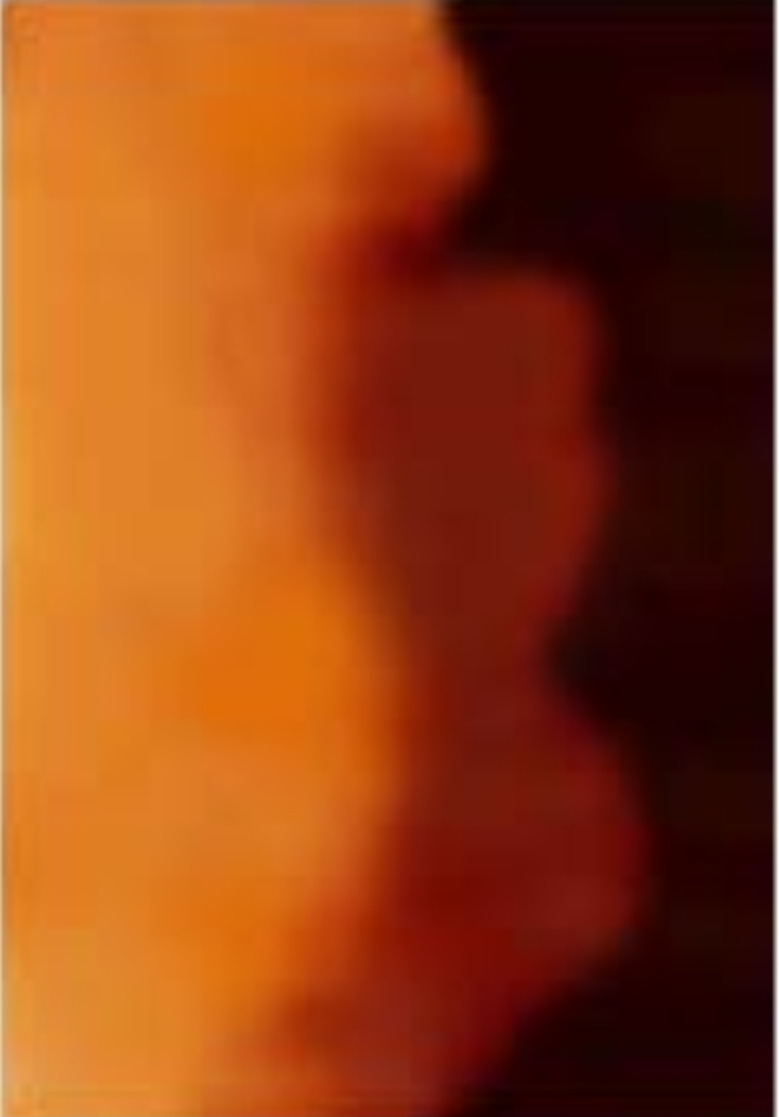
\includegraphics[width = 3.6cm]{Introduction/graphene.png}
\hspace{3cm}
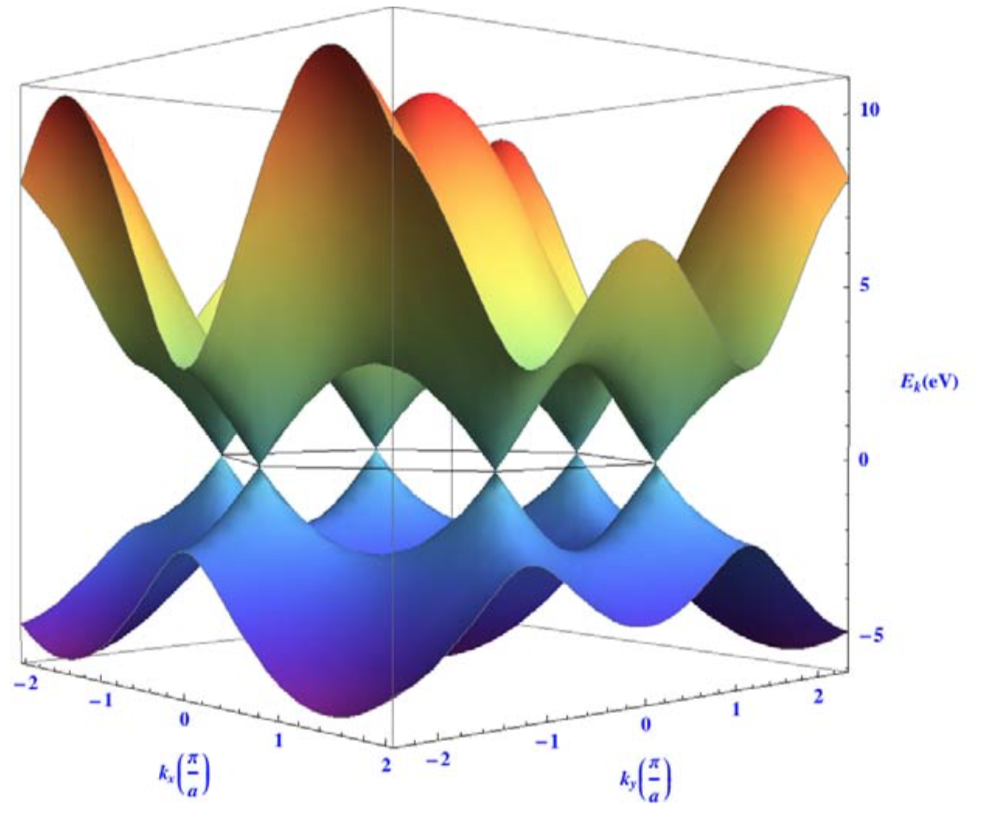
\includegraphics[width = 6.5cm]{Introduction/disp_rel.png}
\caption[Graphene monolayer; graphene's dispersion relation.]{Left: \acf{AFM} picture of a graphene monolayer. The black area is a substrate used for fabrication purposes. The dark orange area is a monolayer of graphene. Right: Dispersion relation of graphene. The black line represents the Fermi energy. Close to it, the dispersion relation is linear, corresponding to massless excitations (taken from \cite{noauthor_nobel_nodate}). }
\label{fig:graphene}
\end{figure}	

On the other hand, \acp{TMD} are a recent member of the \ac{2D} materials family \cite{wang_electronics_2012, roldan_electronic_2014, xu_spin_2014}.
\acp{TMD} have been attracting interest because they seem to overcome some of the drawbacks of graphene in technological applications.
For example, monolayer graphene is gapless, while its bilayer counterpart has only a tunable, but small gap of the order of a tenth of an $eV$.
Contrastingly, \acp{TMD} have an intrinsic gap in excess of $1 \, eV$, being more promising in designing, for example, transistors.
Hole-doped \acp{TMD} are expected to show topological superconductivity \cite{hsu_topological_2017}, while the superconducting phase of graphene has been predicted, but is not easily attained.
Superconductivity in graphene-like \ac{2D} materials is important because it could boost high speed nanoelectronics.
Moreover, the presence of transition metal atoms in \acp{TMD} suggests the possibility of magnetic ordering \cite{braz_valley_2017}, which could be very relevant in nanospintronics applications.
Both topological superconductivity and magnetic ordering arise due to the effect of strong electron correlations.
Thus, to investigate these properties of \acp{TMD} when performing simulations, we need a computational method that is robust enough to capture the effects of electron interactions.

A nanoribbon consists of a \ac{2D} layer that can be regarded as infinitely long on one direction, but not on the other (Figure \ref{fig:fabrication}), so that edge states become relevant, and can be controlled to yield interesting properties.
For simulation purposes, it is natural to assume translational invariance along the ribbon's longitudinal direction, and use \acp{PBC}.
On the other direction, we use \acp{OBC}, effectively considering zigzag edges (Figure \ref{fig:nanoribbons}, left).

\begin{figure}[H]
\centering
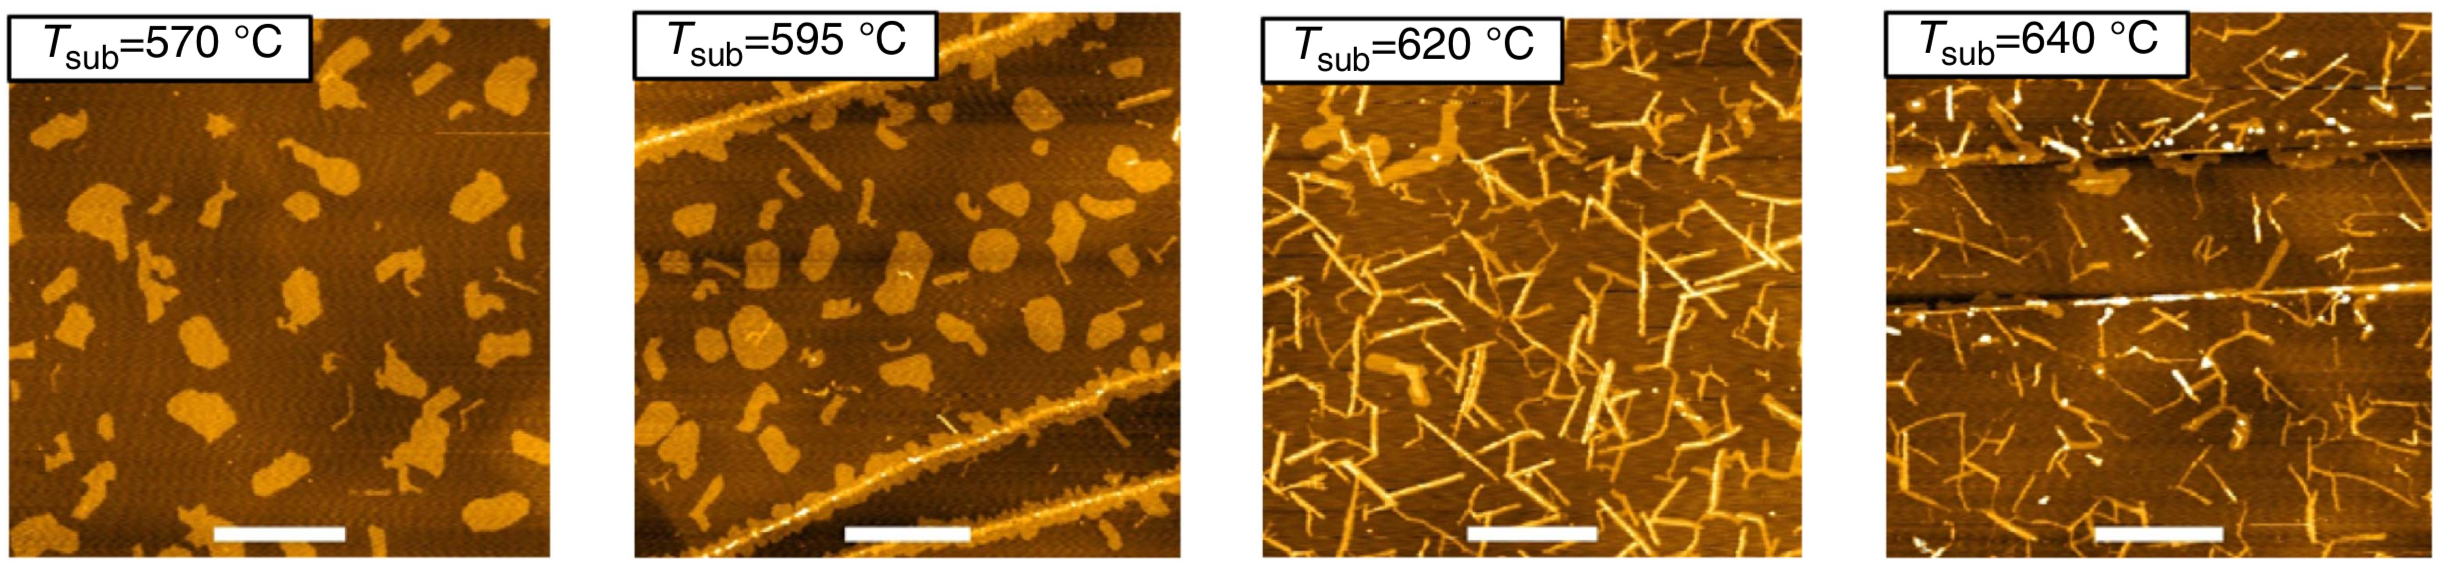
\includegraphics[scale = 0.35]{Introduction/nanoribbons}
\caption[Fabrication of \ac{TMD} nanoribbons]{Fabrication of \ac{TMD} nanoribbons. From left to right, we see \ac{AFM} images showing the appeareance of nanostructures ranging from \ac{2D} nanoislands to nanoribbons, as the temperature of the substrate is increased. The nanoribbons are grown by taking advantage of the temperature dependence of shape transformations occuring during the nonequilibrium growth of this kind of surface-based nanostructures. (taken from \cite{chen_fabrication_2017})}
\label{fig:fabrication}
\end{figure}
   
A high density of low-energy electronic states is localized at the zigzag edges, decaying quickly in the bulk, which suggests the possibility of magnetic ordering.
In fact, a mean field solution of the Hubbard model for a graphene nanoribbon shows that magnetic moments are localized at the edges \cite{yazyev_emergence_2010} (Figure \ref{fig:nanoribbons}, right).
QMC has been used to investigate edge-state magnetism beyond mean field in graphene \cite{feldner_dynamical_2011, golor_quantum_2013, cheng_strain-induced_2015, raczkowski_interplay_2017, yang_strain-tuning_2017}.
However, edge magnetism in TMD nanoribbons remains unexplored \cite{davelou_nanoribbon_2017}.
 
\begin{figure}[H]
\hspace{2cm}
\begin{minipage}[c]{0.1\textwidth}
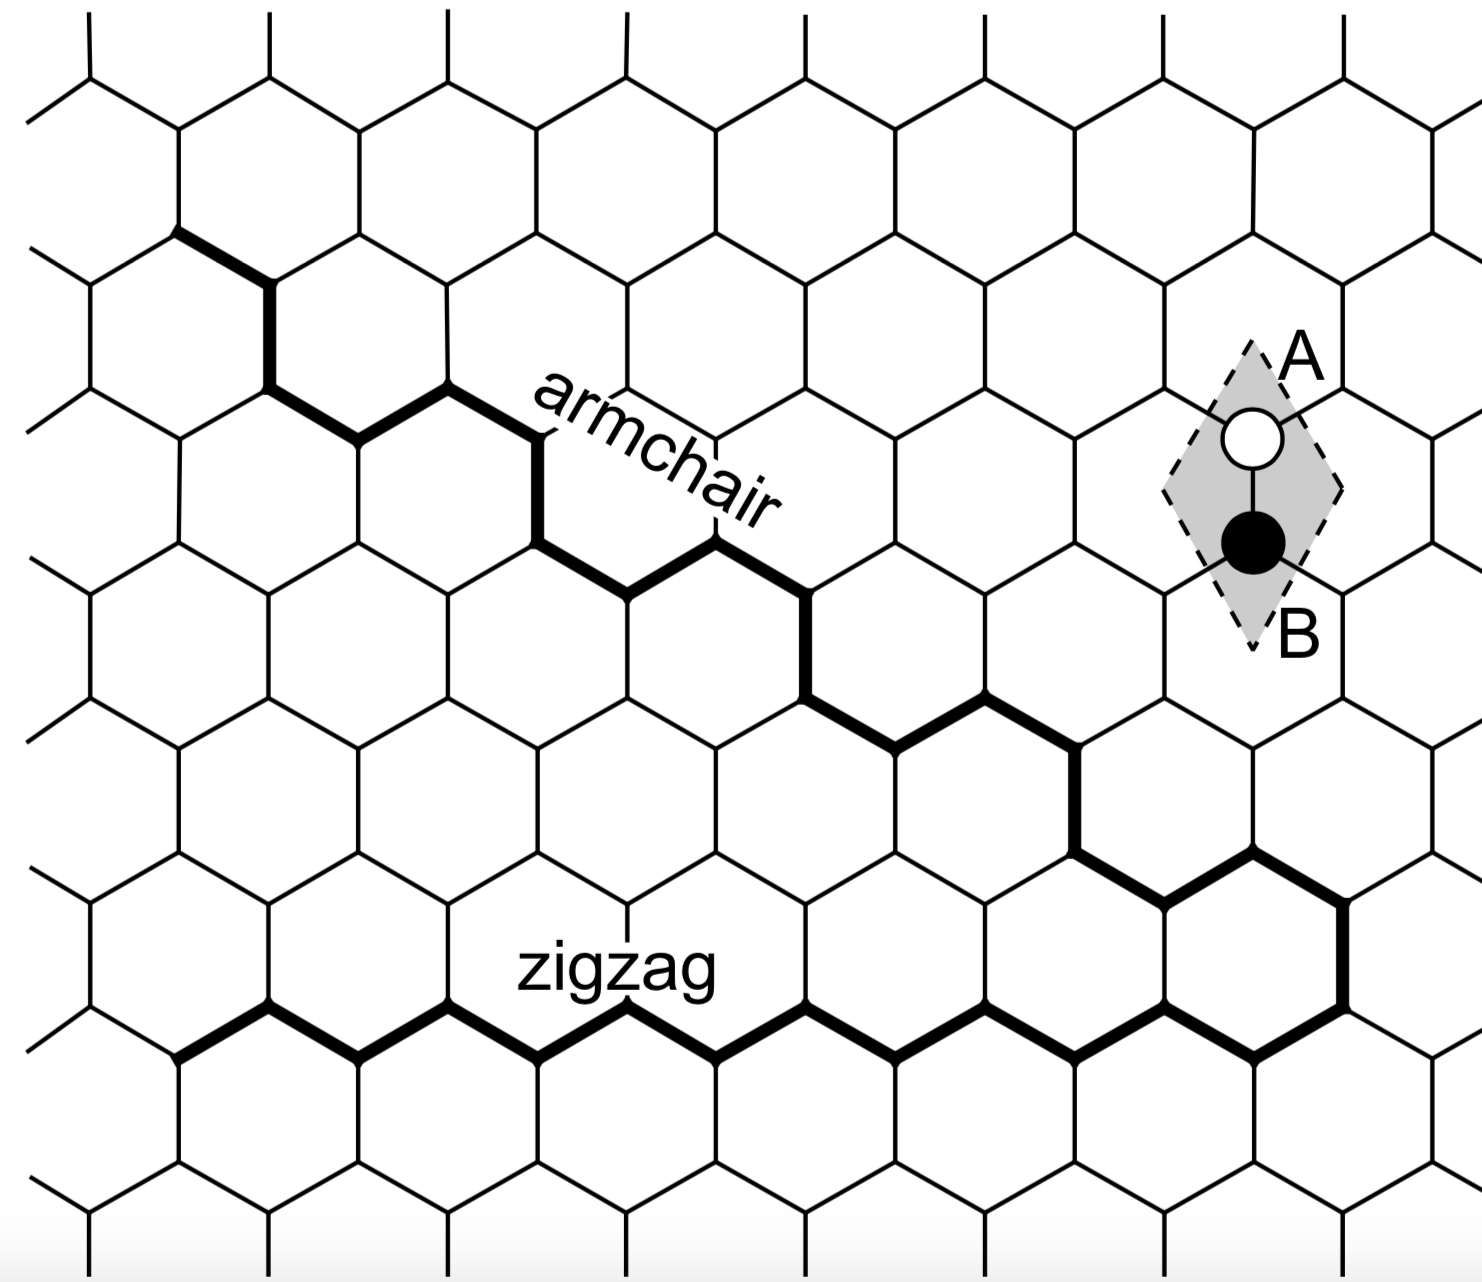
\includegraphics[scale = 0.22]{Introduction/zigzag}
\end{minipage} \hspace{6cm}
\begin{minipage}[c]{0.1\textwidth}
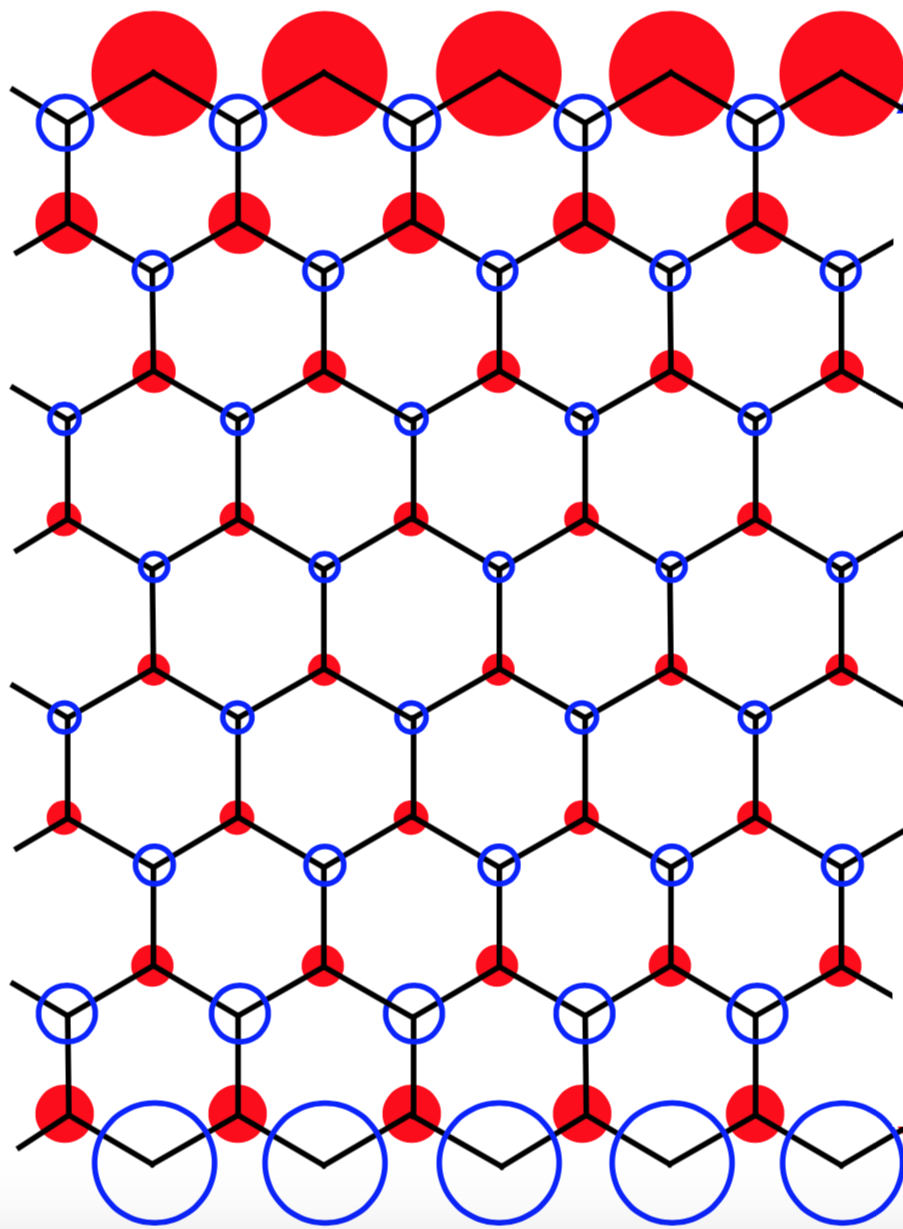
\includegraphics[scale = 0.23]{Introduction/edge_states}
\end{minipage}
 \caption[Zigzag edges of a nanoribbon and magnetism.]{Left: Two possible terminations of a \ac{TMD} nanoribbon condensing in a honeycomb lattice. Right: Local magnetic moments exist on the zig zag edges. The area of the circles corresponds to the magnitude of the magnetic moment, while the color red corresponds to a spin up density, and blue to a spin down density. The accumulation of electronic edge states leads to an \ac{AF} ground state (opposite edges with opposite magnetic moment). (taken from \cite{yazyev_emergence_2010}) \label{fig:nanoribbons}}
\end{figure}

While the zigzag graphene nanoribbon antiferromagnetic ground state is semiconducting, a state with interedge ferromagnetic orientation is a metal.
An example of an application based on the switching between the two states is a magnetorresistive sensor.
This device allows switching between low and high-resistance configurations, corresponding, respectively, to parallel, and antiparallel configurations of ferromagnetic leads at the ends of a nanoribbon.
An important application of this project is precisely the investigation of the possibility of edge-state magnetism, as is observed in graphene nanoribbons, for TMD nanoribbons, which could yield similarly innovative applications.


\subsection{Introduction to \acl{QMC}}

In principle, the properties of a quantum many-fermion system can all be deduced by solving an extremely complicated Schr\"odinger equation that takes into account the coupling of all (identical) particles of the system.
However, for the majority of systems the resulting integrals have no analytic solution, so we solve the problem by numerical integration.
But there is a myriad of methods to evaluate integrals numerically.
How do we pick the best one for this case? 
Multi-dimensional integrals are plagued by the curse of dimensionality.
Although the Newton-Cotes quadrature formulas (including, for example the Newton method, and Simpson's rules), Gaussian quadrature formulas, or Romberg's method all scale polynomially with the number of integration points, they become impractical as the dimension increases.
To use them, one would invoke Fubini's theorem to reduce the multi-dimensional integral to a series of one-dimensional integrals.
However, the number of function evaluations required to compute the whole integral grows exponentially with its dimension.
The Monte Carlo method preserves the polynomial scaling, thus yielding comparable accuracy with far less function evaluations.
It is natural to use it since typically the state space of our quantum system is huge, leading to high dimensional integrals.

The Monte Carlo method is ubiquitous.
Its central idea is to use randomness to produce accurate estimates of deterministic integrals.
The term was coined by Nicolas Metropolis in 1949, first appearing in a seminal paper, in which it was described as a \say{statistical approach to the study of differential equations, or more generally, of integro-differential equations that occur in various branches of sciences}\cite{metropolis_monte_1949}.
Although it was used as early as 1777 in an experiment known as Buffon's needle - where one obtains an estimate of the constant $\pi$ by repeatedly throwing a needle randomly onto a sheet of paper with evenly spaced lines - it was crucially developed in the Los Alamos National Laboratory during World War II where the development of the first atomic bomb was completed, the primary objective of the Manhattan Project.
The method is particularly useful when one wants to sample from a probability distribution in an exponentially large state space.
In fact, it can in principle be used to solve any problem allowing a probabilistic formulation.

A variety of \acf{QMC} methods exists, using a sampling scheme based on the Metropolis algorithm, and variations thereof.
Variational and Diffusion \ac{QMC} are the simplest \ac{QMC} methods that allow one to capture some properties of correlated systems.
Although they already contain the main concepts used in this type of simulations, it is not always possible to use them. 
We will discuss their flaws and show how further refinement leads to the determinant, or auxiliary field method we ultimately used.

Using the Monte Carlo approach to study a many-fermion system implies overcoming a significant obstacle common to all \ac{QMC} methods - the so called \emph{fermion-sign problem}.
Pauli's exclusion principle implies that the many-fermion wave function is anti-symmetric, which leads to a sign oscillation that greatly impedes the accurate evaluation of averages of quantum observables.
The anti-symmetry constraint implies that a  straightforward weight interpretation of the wave function is not possible.
In the case of the finite temperature algorithm, the cancellations that occur when computing the average of any physical observable lead to poor statistical properties of the corresponding estimators.
This means that a massive amount of samples requiring enormous computer time are needed to obtain meaningful results.
In the case of the zero temperature algorithms, the situation is even worse.
It might not even be possible to design a stochastic process carrying the system to its ground state, as normally is done in \say{projective} methods\footnote{Methods that iteratively project a trial wave function onto the ground state.}: the wave function that is used as an initial proposal turns out to converge to a bosonic one, and the fermionic character of the system is lost.

As was proven by Troyer, the \emph{fermion-sign problem} has NP\footnote{NP or nondeterministic polynomial time, meaning that one can devise an algorithm that verifies the "yes" answer to a decision problem in polynomial time in the system size.
Note that the class $P$ - of polynomial time algorithms - is a subclass of NP.} computational complexity \cite{troyer_computational_2005}.
One of the greatest open questions in computer science is whether $P = NP$.
Solving the \emph{fermion-sign problem} would imply finding a solution to $P = NP$, which would constitute a major breakthrough.



\subsection{Variational Monte Carlo}

Variational techniques rely on an educated guess for the wave function of the system.
One introduces a set of variational parameters $\bm \alpha$ that are then tuned according to a variational principle.
Then, we may use the optimized trial wave function to compute physical quantities of interest using Monte Carlo.
The method is used to obtain zero temperature properties of a given model.
Note that it requires prior knowledge about the system to propose an approximate wave function in the first place.

A particularly relevant observable is the variational energy $E_V$ associated to a trial ground state.
Let $\bm r$ be the $3N$ spatial coordinates of the $N$ electrons.
Given the Hamiltonian of the system $\mathcal{H}$, and a trial wave function $\psi (\bm r)$ - a guess of the wave function representing the ground state - one can compute the corresponding variational energy.

\begin{equation}\label{eq:variational_energy}
E_V = \frac{\left\langle \psi | \mathcal{H} | \psi \right \rangle}{\left\langle \psi | \psi \right \rangle} = \frac{ \int d\bm r |\psi (\bm r)|^2 E_L (\bm r)}{\int d\bm r | \psi (\bm r)|^2 } = \int d\bm r\rho (\bm r) E_L (\bm r) ,
\end{equation}
where the local energy $E_L (\bm r)$ is defined as

\begin{equation}\label{eq:local_energy}
E_L = \frac{\mathcal{H} \psi (\bm r) }{\psi (\bm r)}
\end{equation}
and the probability distribution $\rho (\bm r)$ is defined as

\begin{equation}\label{eq:rho}
\rho (\bm r) = \frac{ | \psi (\bm r) |^2}{ \int d\bm r' | \psi (\bm r') |^2}
\end{equation}

Note that we managed to recast the variational energy as an average of the \emph{local} energy, $\left\langle E_L \right\rangle $, over the the distribution $\rho$.
This may be computed using the Monte Carlo method by sampling $M$ points $\bm r_k$ from distribution $\rho (\bm r)$:

\begin{equation}\label{eq:average}
E_V \approx \overline{E}_L = \frac{1}{M} \sum_{k= 1}^{M} E_L (\bm r_k) ,
\end{equation}
where $\overline {X}$ denotes a sample mean of the random variable $X$.

Let the ground state energy be $E_0$.
Then, states are optimized according to the variational principle:

\begin{equation}
E_V(\bm \alpha) = \frac{\left\langle \psi_{\bm \alpha} | \mathcal{H} | \psi_{\bm \alpha} \right\rangle}{\left\langle\psi_{\bm \alpha} | \psi_{\bm \alpha} \right\rangle} \ge E_0,
\end{equation}
where $\psi_{\bm \alpha}$ is the trial ground state wave function for the set of variational parameters ${\bm \alpha}$.

By varying $\bm \alpha$ we aim to obtain a variational energy that is as close as possible to the true ground state energy.
Since $E_V(\bm \alpha)$ is bounded from below, this is equivalent to minimizing it in the hope that $E_V(\bm \alpha_{min}) \gtrsim E_0$, i.e. the bound is tight.

The finite sampling size $M$, of course, introduces a statistical error common to all Monte Carlo methods. 
However, the use of an approximate wave function introduces a systematic error that is hard to control since trial wave functions are generally introduced based on approximate, or heuristic arguments.

\subsection{Diffusion Monte Carlo and projective methods}\label{subsec:dmc}

Variational Monte Carlo is severely limited by the use of a trial wave function $\psi_{\bm \alpha} (\bm r)$ because we may even not have enough information to even construct a reliable variational wave function.

Diffusion \ac{QMC} allows the simulation of a many-body system while having only a limited knowledge of the system's physical properties.
While it is exact for many-boson systems, it is only approximate for many-fermion systems.
The idea is to map the Schr\"odinger equation into  an imaginary-time diffusion equation.
Excited states are then filtered out by a diffusion process as we advance in imaginary-time.
In imaginary-time $\tau = i t$, the solution to the Schr\"odinger equation in terms of a formal series expansion in the eigenfunctions of the hamiltonian becomes a series of transients $e^{-E_n \tau}, \, n \in \mathbb{N}$.
The longest lasting of these is the ground state  \cite{kosztin_introduction_1996}.

The idea of the diffusion method is to generate samples using the exact ground state wave function $\psi_0 (\bm r)$ \cite{toulouse_chapter_2016}.
The associated exact energy $E_0$ is the matrix element of the hamiltonian calculated using a trial wave function and the ground state wave function.

\begin{equation}
E_0 = \frac{ \left\langle \psi_0 |E_0 \mathbbm{1} | \psi \right\rangle}{\left\langle \psi_0 | \psi \right\rangle} = \frac{\left\langle \psi_0 | \mathcal{H} | \psi \right\rangle}{ \left\langle\psi_0 | \psi \right\rangle} = \frac{\int d\bm r \psi_0^\star (\bm r) \psi (\bm r) E_L (\bm r)}{\int d\bm r\psi_0^\star (\bm r) \psi (\bm r)}
\end{equation}

Note that using this trick we avoid the computation of $\mathcal{H} \psi_0 = E_0 \psi_0$, that is, the ground state energy.
Instead, we approximate the integral by considering $M$ configuration samples $\bm r_{k = 1,..., N}$ in a similar spirit to that of Variational \ac{QMC}.
Notice that the integral consists of a local energy of the trial wave function $E_L (\bm r) = \frac{\mathcal{H} \psi (\bm r)}{\psi (\bm r)}$ averaged over a mixed distribution from which we draw a sample of points $\bm r_{k=1,...M}$:

\begin{equation}
f(\bm r) = \frac{\psi_0^\star (\bm r) \psi (\bm r) }{ \int d\bm r  \psi_0 (\bm r) \psi (\bm r)}
\end{equation}

Although the method is, of course, aimed at probing many-body systems, let us consider a single particle in \acs{1D} for simplicity for illustrating the method.
Performing a Wick rotation - effectively going to imaginary time - and shifting the energy, the Schr\"odinger equation becomes

\begin{equation}
\frac{\partial \psi ( x, \tau )}{\partial\tau}  = -\frac{1}{2m}\frac{\partial^2 \psi ( x, \tau )}{\partial x^2} - \bigg[ V(x) - E_T \bigg] \psi( x, \tau ) 
\end{equation}

The exact ground state wave function $\psi_0 ( x )$ is obtained as the longest lasting transient state in imaginary time: we are interested in the asymptotic behavior of the series expansion constituting the formal solution of the Schr\"odinger equation

\begin{equation}
\psi (x, \tau) = \sum_{n=0}^{\infty} c_n \psi_n (x) e^{-(E_n - E_T)\tau}
\end{equation}

Imaginary time evolution is governed by

\begin{equation}\label{eq:im_ev}
\begin{split}
&\left| \psi (t) \right\rangle = \lim_{\tau \rightarrow \infty} \sum_i e^{-(E_i - E_T) \tau} \left|\psi_i \right\rangle \left\langle \psi_i | \psi \right\rangle = \\
&= \lim_{\tau \rightarrow \infty} e^{-(E_0 - E_T)\tau} \left| \psi_0 \right\rangle \left\langle \psi_0 | \psi \right\rangle 
\end{split}
\end{equation}


If $E_T > E_0$ the wave function diverges exponentially fast: $\lim_{\tau \rightarrow \infty} \psi ( x, \tau) = \infty$.
Similarly, for $E_T < E_0$ it vanishes exponentially fast: $\lim_{\tau \rightarrow \infty} \psi ( x, \tau) = 0$.
However, if $E_T = E_0$ the wave function converges to the ground state one up to a constant factor.

\begin{equation}\label{eq:dmc}
\lim_{\tau \rightarrow \infty} \psi ( x, \tau) = c_0 \psi_0 (x) \,\,\, \text{, or} \quad \lim_{\tau \rightarrow \infty} \left|\psi (\tau) \right\rangle \propto \left| \psi_0 \right\rangle
\end{equation}

Diffusion \ac{QMC} makes use of Eq. (\ref{eq:dmc}), approximating $\psi_0(x)$ by $\psi (x, \tau)$ for sufficiently long time.
The only requirement is that $\psi (x, \tau)$ and $\psi_0(x)$ overlap significantly so that $c_0$ is large enough to be numerically measurable, and we can always center a positive trial wave function in a region where $\psi_0(x)$ is large enough and positive.
If the latter condition does not hold, the wave function converges to a bosonic, instead of a fermionic one.
Of course, these conditions can always be met for a single particle, but note that they might fail for a many-fermion system, for which the wave function crosses a number of nodes due to its anti-symmetric nature.

\subsection{Drawbacks of variational and projective methods. Auxiliary Field \acs{QMC}. The Fermion Sign Problem.}
\label{subsec:introAFQMC}

As we have seen, the major drawback of the variational method was that it demanded \emph{a priori} knowledge of a reasonable variational wave function describing, at least partly, some of the physics of the problem.
Diffusion \acs{QMC} demands less: we need only propose a trial wave function that overlaps with the ground state.
However, none of these methods allow us to probe systems at finite temperature.
Moreover, they both require some prior knowledge about the system, which may not always be available.

An alternative method is based on introducing an additional lattice bosonic field that mediates the electron-electron interaction.
The interacting problem then becomes a problem of independent fermions coupled to an external field, and the fermionic part of the partition function can be traced out explicitly, leaving the contribution of a \emph{discrete}\footnote{Although, there is a finite number of field configurations, the number grows exponentially with the number of sites on the lattice.} bosonic field.
This contribution can be evaluated numerically by employing importance sampling over the field configurations.
Auxiliary field \acs{QMC} relies on a mapping to a classical system:

\begin{equation}
Z = \Tr [ e^{-\beta \mathcal{H} } ] = \sum_c p_c ,
\end{equation}
but some of the \say{probabilities} can actually be negative $p_c < 0$.
This occurs due to the antisymmetry of the many-electron wave function under exchange of two electrons.

The negative weight problem may easily be circumvented when computing averages of observables:

\begin{equation}\label{eq:signSampling}
\left\langle A \right\rangle = \frac{\sum_c A ( c ) p ( c )}{\sum_c p ( c ) } = \frac{\sum_c A ( c )|  p ( c ) | \text{sign}[p(c)] / \sum_c | p ( c ) | }{\sum_c  |  p ( c ) | \text{sign}[p(c)] /  \sum_c | p ( c ) |} \equiv \frac{\left\langle A s \right\rangle_{|p|}}{\left\langle s \right\rangle_{|p|}} ,
\end{equation}
where $s(c) = \text{sign} [ p ( c ) ]$, and $| p ( c ) | $ corresponds to an auxiliary bosonic system (also coupled to the bosonic field) corresponding to the original fermionic system, and for which there is no sign problem.

The relative error $\Delta s / \left\langle s \right\rangle$ increases exponentially with the number of particles, with inverse temperature, and possibly with other parameters of the specific model to be studied \cite{troyer_computational_2005, hou_numerical_2009}.
To see this, we start by noting that the average sign is the ratio between the partition functions of the fermionic ($Z = \sum_c p(c)$) and bosonic systems ($Z = \sum_c | p ( c ) |$).
In terms of the difference in free energy densities, $\left\langle s \right\rangle = Z / Z' = e^{-\beta N_p \Delta f}$, implying that for $M$ samples, the error of the denominator of Eq. (\ref{eq:signSampling}) becomes

\begin{equation}
\frac{\Delta s}{\left\langle s \right\rangle} = \frac{\sqrt{(\left\langle s^2 \right\rangle - \left\langle s \right\rangle^2 )/ M }}{\left\langle s \right\rangle} = \frac{ \sqrt{ 1 - \left\langle s \right\rangle^2}  }{\sqrt{M} \left\langle s \right\rangle} \propto \frac{e^{\beta N_p \Delta f}}{\sqrt{M}} ,
\end{equation}
and similarly for the numerator of Eq. (\ref{eq:signSampling}).

Auxiliary field \acs{QMC} can also be formulated to probe ground state properties, and a sign problem arises similarly.
Apart from this problem, which plagues all \acs{QMC} methods, this method is one of the most robust, unbiased, and reliable methods, hence we choose it to carry out our simulations.
Note that, in particular, it is certainly more powerful than the variational and diffusion methods outlined before since it requires much less \emph{a priori} information about the system.
Perhaps more importantly, given some recent findings, it can be used in conjunction with neural networks to discover quantum phase transitions in correlated systems  \cite{broecker_machine_2017}.
\section{Introduction to \acl{QMC}}
\label{sec:introQMC}

Solving the many-body problem remains one of the greatest challenges in physics.
Following the wealth of attempts at such pursuit, certain phenomena arising due to the strong interactions in quantum systems are explained in different theoretical frameworks, namely superconductivity, the Mott metal-insulator transition, and fractional quantum Hall effect.
All of these breakthroughs represented revolutions in their respective fields with significant scientific and technological impact.
However, only in very limited cases does an actual analytical solution exist for the  Schr\"odinger equation for a system of interacting particles.
One must resort to sophisticated approximation methods to obtain  information about the role played by the competing interactions under various conditions in the aforementioned cases.
It is then natural that numerical methods have become prominent as a tool for extracting useful information about this type of systems.
\ac{QMC} is amongst the most accurate and extensively studied ones.
The idea of all \ac{QMC} methods is to reduce the interacting problem to solving a set of integrals, which can be evaluated numerically through a standard stochastic procedure.
These integrals are arrived at upon formulating the quantum many-body description of the system using the Schr\"odinger equation.
Hence the name \acl{QMC}, which is used to distinguish it from Classical Monte Carlo.
In the classical version, one measures thermal averages, while in the quantum version, one measures expectations of operators over the Hilbert space of the system, corresponding to physical observables that fluctuate with a dynamics given by the Schr\"odinger equation (and, of course, can also have thermal fluctuations).
In fact, the dynamics of a quantum system are encoded in the Hamiltonian operator.
In the case of graphene-like \ac{2D} materials, one usually uses a tight-binding model.
It is found that the dynamics given by the tight-binding Hamiltonian is sufficient to describe most properties of graphene.
However, in other materials, such as \acp{TMD}, electron-electron interactions are stronger, and Hubbard-type models could give us a more accurate picture of the phenomena that occur within them.

For quantum many-fermion systems, observables are given in terms of integrals which have no analytic solution, so we solve the problem numerically.
But there is a myriad of methods to evaluate integrals numerically.
How do we pick the best one for this case? 
Multi-dimensional integrals are plagued by the curse of dimensionality.
Although the Newton-Cotes quadrature formulas (including, for example the Newton method, and Simpson's rules), Gaussian quadrature formulas, or Romberg's method all scale polynomially with the number of integration points, they become impractical as the dimension increases.
To use them, one would invoke Fubini's theorem to reduce the multi-dimensional integral to a series of one-dimensional integrals.
However, the number of function evaluations required to compute the whole integral grows exponentially with its dimension.
The Monte Carlo method preserves the polynomial scaling, thus yielding comparable accuracy with far less function evaluations.
It is natural to use it since typically the state space of our quantum system is huge, leading to high dimensional integrals.

The Monte Carlo method is ubiquitous.
Its central idea is to use randomness to produce accurate estimates of deterministic integrals.
The term was coined by Metropolis in 1949, although it was used as early as 1777 in an experiment known as Buffon's needle - where one obtains an estimate of the constant $\pi$ by repeatedly throwing a needle randomly onto a sheet of paper with evenly spaced lines. %t was crucially developed in the Los Alamos National Laboratory during World War II where the development of the first atomic bomb was completed, the primary objective of the Manhattan Project.
The method is particularly useful when one wants to sample from a probability distribution in an exponentially large state space (like the huge Hilbert space of an interacting electron system), but it can, in principle, be used to solve any problem allowing a probabilistic formulation.
To solve the interacting fermion problem, a variety of \ac{QMC} methods exists, using a sampling scheme based on the Metropolis algorithm, and variations thereof.
Variational and Diffusion \ac{QMC} are the simplest \ac{QMC} methods that allow one to capture some properties of correlated systems, but it is not always ideal or even possible to use them. 
%We will discuss their flaws and show how further refinement leads to the auxiliary field method we ultimately used.

Using the Monte Carlo approach to study a many-fermion system implies overcoming a significant obstacle common to all \ac{QMC} methods - the so called \emph{fermion sign problem}.
Pauli's exclusion principle implies that the many-fermion wave function is anti-symmetric, which leads to a sign oscillation that greatly impedes the accurate evaluation of averages of quantum observables.
The anti-symmetry constraint implies that a  straightforward weight interpretation of the wave function is not possible.
In the case of the finite temperature algorithm, the cancellations that occur when computing the average of any physical observable lead to poor statistical properties of the corresponding estimators.
This means that a massive amount of samples requiring enormous computer time are needed to obtain meaningful results.
In the case of the zero temperature algorithms, the situation is even worse.
It might not even be possible to design a stochastic process carrying the system to its ground state, as normally is done in \say{projective} methods\footnote{Methods that iteratively project a trial wave function onto the ground state.}: the wave function that is used as an initial proposal turns out to converge to a bosonic one, and the fermionic character of the system is lost.
As was proven by Troyer, the \emph{fermion sign problem} has NP\footnote{NP or nondeterministic polynomial time, meaning that one can devise an algorithm that verifies the "yes" answer to a decision problem in polynomial time in the system size.
Note that the class $P$ - of polynomial time algorithms - is a subclass of NP.} computational complexity \cite{troyer_computational_2005}.
One of the greatest open questions in computer science is whether $P = NP$.
Solving the \emph{fermion sign problem} would imply finding a solution to $P = NP$, which would constitute a major breakthrough.

\subsection{Variational Monte Carlo}

Variational techniques rely on an educated guess for the wave function of the system.
One introduces a set of variational parameters $\bm \alpha$ that are then tuned according to a variational principle.
Then, we may use the optimized trial wave function to compute physical quantities of interest using Monte Carlo.
The method is used to obtain zero temperature properties of a given model.
Note that it requires prior knowledge about the system to propose an approximate wave function in the first place.

A particularly relevant observable is the variational energy $E_V$ associated to a trial ground state.
Let $\bm r$ be the $3N$ spatial coordinates of the $N$ electrons.
For simplicity, let us ignore all other degrees of freedom, such as spin.
Given the Hamiltonian of the system $\mathcal{H}$, and a trial wave function $\psi_T (\bm r)$ - a guess of the wave function representing the ground state - one can compute the corresponding variational energy by averaging over a \say{local} energy:

\begin{equation}\label{eq:variational_energy}
E_V = \frac{\left\langle \psi_T | \mathcal{H} | \psi_T \right \rangle}{\left\langle \psi_T | \psi_T \right \rangle} = \frac{ \int d\bm r |\psi_T (\bm r)|^2 E_L (\bm r)}{\int d\bm r | \psi_T (\bm r)|^2 } = \int d\bm r\rho (\bm r) E_L (\bm r) , \text{where}
\end{equation}

\begin{equation}\label{eq:local_energy}
E_L = \frac{\mathcal{H} \psi_T (\bm r) }{\psi_T (\bm r)}   \quad \text{and} \quad \rho (\bm r) = \frac{ | \psi_T (\bm r) |^2}{ \int d\bm r' | \psi_T (\bm r') |^2}
\end{equation}

Note that we managed to recast the variational energy as an average of the \emph{local} energy, $\left\langle E_L \right\rangle $, over the the distribution $\rho$.
This may be computed using the Monte Carlo method by sampling $M$ points $\bm r_k$ from the distribution $\rho (\bm r)$.
Denoting the sample mean of the random variable $X$ as $\overline {X}$:

\begin{equation}\label{eq:average}
E_V \approx \overline{E}_L = \frac{1}{M} \sum_{k= 1}^{M} E_L (\bm r_k) ,
\end{equation}

Let the ground state energy be $E_0$.
Then, states are optimized according to the variational principle:

\begin{equation}
E_V(\bm \alpha) = \frac{\left\langle \psi_{\bm \alpha} | \mathcal{H} | \psi_{\bm \alpha} \right\rangle}{\left\langle\psi_{\bm \alpha} | \psi_{\bm \alpha} \right\rangle} \ge E_0,
\end{equation}
where $\psi_{\bm \alpha}$ is the trial ground state wave function for the set of variational parameters ${\bm \alpha}$.
By varying $\bm \alpha$ we aim to obtain a variational energy that is as close as possible to the true ground state energy, and use the corresponding trial wave function to compute averages of other observables.
Since $E_V(\bm \alpha)$ is bounded from below, this is equivalent to minimizing it in the hope that $E_V(\bm \alpha_{min}) \gtrsim E_0$, i.e. the bound is tight.
The finite sampling size $M$, of course, introduces a statistical error common to all Monte Carlo methods. 
However, the use of an approximate wave function introduces a systematic error that is hard to control since trial wave functions are generally introduced based on approximate, or heuristic arguments.

\subsection{Diffusion Monte Carlo and projective methods}\label{subsec:dmc}

Variational Monte Carlo is severely limited by the use of a trial wave function $\psi_T (\bm r)$ because we may not even have enough information to even construct a reliable variational wave function in the first place.
Diffusion \ac{QMC} allows the simulation of a many-body system while having only a limited knowledge of the system's physical properties.
As a projective method, it is exact for many-boson systems, while being only approximate for many-fermion systems.
The idea is to map the Schr\"odinger equation onto an imaginary-time diffusion equation.
Excited states are then filtered out by a diffusion process as we advance in imaginary-time.
In imaginary-time $\tau = i t$, the solution to the Schr\"odinger equation in terms of a formal series expansion in the eigenfunctions of the Hamiltonian becomes a series of \say{transient} wavefunctions weighted by $e^{-E_n \tau}, \, n \in \mathbb{N}$.
Within precision and accuracy constraints, the longest lasting of these is the ground state \cite{kosztin_introduction_1996}.
Thus, the idea of the diffusion method is to generate samples using the exact ground state wave function $\psi_0 (\bm r)$ \cite{toulouse_chapter_2016}.
The associated exact energy $E_0$ is the matrix element of the hamiltonian calculated using a trial wave function and the ground state.

\begin{equation}
E_0 = \frac{ \big( \left\langle \psi_0 |E_0 \big) \big( \mathbbm{1} | \psi_T \right\rangle \big)}{\left\langle \psi_0 | \psi_T \right\rangle} = \frac{\left\langle \psi_0 | \mathcal{H} | \psi_T \right\rangle}{ \left\langle\psi_0 | \psi_T \right\rangle} = \frac{\int d\bm r \psi_0^\star (\bm r) \psi_T (\bm r) E_L (\bm r)}{\int d\bm r\psi_0^\star (\bm r) \psi_T (\bm r)}
\end{equation}

Note that using this trick we avoid the computation of $\mathcal{H} \psi_0 = E_0 \psi_0$, that is, the ground state energy.
Instead, we approximate the integral by considering $M$ configuration samples $\bm r_{k = 1,..., M}$ in a similar spirit to that of Variational \ac{QMC}.
Notice that the integral consists of a local energy of the trial wave function $E_L (\bm r) = \frac{\mathcal{H} \psi (\bm r)}{\psi (\bm r)}$ averaged over a mixed distribution from which we draw a sample:

\begin{equation}
f(\bm r) = \frac{\psi_0^\star (\bm r) \psi_T (\bm r) }{ \int d\bm r  \psi_0 (\bm r) \psi_T (\bm r)}
\end{equation}

Although the method is, of course, aimed at probing many-body systems, let us consider a single particle in \acs{1D}, for simplicity, to illustrate the method.
Performing a Wick rotation - effectively going to imaginary time - and shifting the energy, the Schr\"odinger equation becomes (with $\hbar = 1$)

\begin{equation}
\frac{\partial \psi_T ( x, \tau )}{\partial\tau}  = -\frac{1}{2m}\frac{\partial^2 \psi_T ( x, \tau )}{\partial x^2} - \bigg[ V(x) - E_T \bigg] \psi_T( x, \tau ) 
\end{equation}

The exact ground state wave function $\psi_0 ( x )$ is obtained as the longest lasting transient state in imaginary time: we are interested in the asymptotic behavior of the series expansion constituting the formal solution of the Schr\"odinger equation

\begin{equation}
\psi_T (x, \tau) = \sum_{n=0}^{\infty} c_n \psi_n (x) e^{-(E_n - E_T)\tau}
\end{equation}

Imaginary time evolution is governed by

\begin{equation}\label{eq:im_ev}
\left| \psi_T (t) \right\rangle = \lim_{\tau \rightarrow \infty} \sum_n e^{-(E_n - E_T) \tau} \left|\psi_n \right\rangle \left\langle \psi_n | \psi_T \right\rangle = \lim_{\tau \rightarrow \infty} e^{-(E_0 - E_T)\tau} \left| \psi_0 \right\rangle \left\langle \psi_0 | \psi_T \right\rangle 
\end{equation}

If $E_T > E_0$ the wave function diverges exponentially fast: $\lim_{\tau \rightarrow \infty} \psi_T ( x, \tau) = \infty$.
Similarly, for $E_T < E_0$ it vanishes exponentially fast: $\lim_{\tau \rightarrow \infty} \psi_T ( x, \tau) = 0$.
However, if $E_T = E_0$ the wave function converges to the ground state one up to a constant factor, $c_0 = \left\langle \psi_0 | \psi_T \right\rangle$.

\begin{equation}\label{eq:dmc}
\lim_{\tau \rightarrow \infty} \psi_T ( x, \tau) = c_0 \psi_0 (x) \quad \text{or} \quad \lim_{\tau \rightarrow \infty} \left|\psi_T (\tau) \right\rangle \propto \left| \psi_0 \right\rangle
\end{equation}

Diffusion \ac{QMC} makes use of Eq. (\ref{eq:dmc}), approximating $\psi_0(x)$ by $\psi_T (x, \tau)$ for sufficiently long time.
The only requirement is that $\psi_T (x, \tau)$ and $\psi_0(x)$ overlap significantly so that $c_0$ is large enough to be numerically measurable, and we can always center a positive trial wave function in a region where $\psi_0(x)$ is large enough and positive.
If the latter condition does not hold, the wave function converges to a bosonic, instead of a fermionic one.
Of course, these conditions can always be met for a single particle, but note that they might fail for a many-fermion system, for which the wave function crosses a number of nodes due to its anti-symmetric nature.

\subsection{Auxiliary Field \acs{QMC} and the Fermion Sign Problem}
\label{subsec:introAFQMC}

As we have seen, the major drawback of the variational method was that it demanded \emph{a priori} knowledge of a reasonable variational wave function describing, at least partly, some of the physics of the problem.
Diffusion \acs{QMC} demands less: we need only propose a trial wave function that overlaps with the ground state.
However, none of these methods allow us to probe systems at finite temperature.
Moreover, they both require some prior knowledge about the system, which may not always be available.

An alternative method is based on introducing an additional lattice bosonic field that mediates the electron-electron interaction.
The interacting problem then becomes a problem of independent fermions coupled to an external field, and the fermionic part of the partition function can be traced out explicitly, leaving the contribution of a \emph{discrete}\footnote{The introduced field is discrete (and \emph{binary}) because each fermionic state can only have occupations $n = 0, 1$. Although, there is a finite number of field configurations, the number grows exponentially with the number of sites on the lattice.} bosonic field, $\bm h$.
This contribution can be evaluated numerically by employing importance sampling over the field configurations.
Auxiliary field \acs{QMC} relies on a mapping to a so called \say{classical} system (in quotes because there may be no actual classical analogue):

\begin{equation}\label{eq:Zsign}
Z = \Tr [ e^{-\beta \mathcal{H} } ] = \sum_{\{ \bm h\} } \sum_{\text{fermionic}} e^{-S} = \sum_c p_c ,
\end{equation}
but some of the \say{probabilities} can actually be negative $p_c < 0$.
This occurs due to the antisymmetry of the many-electron wavefunction under electron exchange, and is at the root of the sign problem.
Here, $S$ is a fermion-boson action that we shall write out explicitly later.
For a fixed configuration of the bosonic field, we sum over the fermionic part exactly to obtain the weight of each configuration $p_c$.
The sum over $\bm h$ is carried out stochastically.

The negative weight problem may easily be circumvented when computing averages of observables:

\begin{equation}\label{eq:signSampling}
\left\langle A \right\rangle = \frac{\sum_c A ( c ) p ( c )}{\sum_c p ( c ) } = \frac{\sum_c A ( c )|  p ( c ) | \text{sign}[p(c)] / \sum_c | p ( c ) | }{\sum_c  |  p ( c ) | \text{sign}[p(c)] /  \sum_c | p ( c ) |} \equiv \frac{\left\langle A s \right\rangle_{|p|}}{\left\langle s \right\rangle_{|p|}} ,
\end{equation}
where $s(c) = \text{sign} [ p ( c ) ]$, and $| p ( c ) | $ corresponds to an auxiliary bosonic system (also coupled to the bosonic field) corresponding to the original fermionic system, and for which there is no sign problem.

The relative error $\Delta s / \left\langle s \right\rangle$ increases exponentially with the number of particles, with inverse temperature, and possibly with other parameters of the specific model to be studied \cite{troyer_computational_2005, hou_numerical_2009}.
To see this, we start by noting that the average sign is the ratio between the partition functions of the fermionic ($Z = \sum_c p(c)$) and bosonic systems ($Z' = \sum_c | p ( c ) |$).
In terms of the difference in free energy densities, $\left\langle s \right\rangle = Z / Z' = e^{-\beta N_p \Delta f}$, implying that for $M$ samples, the error of the denominator of Eq. (\ref{eq:signSampling}) becomes

\begin{equation}
\frac{\Delta s}{\left\langle s \right\rangle} = \frac{\sqrt{(\left\langle s^2 \right\rangle - \left\langle s \right\rangle^2 )/ M }}{\left\langle s \right\rangle} = \frac{ \sqrt{ 1 - \left\langle s \right\rangle^2}  }{\sqrt{M} \left\langle s \right\rangle} \propto \frac{e^{\beta N_p \Delta f}}{\sqrt{M}} ,
\end{equation}
and similarly for the numerator of Eq. (\ref{eq:signSampling}).

Auxiliary field, or determinant \acs{QMC} can also be formulated to probe ground state properties, and a sign problem arises similarly.
In fact, this problem plagues all \acs{QMC} methods, even though we showed it only for the determinant method\footnote{So called because, as we shall show later, $p_c$ boils down to a product of determinants that depends on the energy scales of the problem.}.
The latter is the most robust, unbiased, and reliable method, with a generally modest sign problem, hence we choose it to carry out our simulations.

Furthermore, in general, it suffices to use the finite temperature auxiliary field  method with $\beta$ large enough to probe ground state properties (for example, this is shown numerically for the Hubbard model on the square lattice in \cite{white_numerical_1989}).
In this case, the inverse temperature may be regarded as being analogous to a  projective parameter $\Theta$, characterizing convergence to the ground state, within statistical uncertainty.
Projector \ac{QMC}, the zero temperature version of auxiliary field \ac{QMC} is based on an equation similar to Eq.(\ref{eq:dmc}).
Any observable $A$ is computed by use of a trial wave function with some overlap with the ground state $\left\langle \psi_T | \psi_0 \right\rangle \neq 0$ (see \cite{f._assaad_quantum_2002} for more details on the projector method; in this work we focus on the finite temperature version since it is more general):

\begin{equation}
\left\langle A \right\rangle = \lim_{\Theta \rightarrow \infty} \frac{\left\langle \psi_T | e^{-\Theta \mathcal{H} } A e^{-\Theta \mathcal{H} } | \psi_T \right\rangle }{\left\langle \psi_T | e^{- 2 \Theta \mathcal{H} } | \psi_T \right\rangle}
\end{equation}

Note that auxiliary field \ac{QMC} is more powerful than the variational and diffusion methods outlined before since it requires much less \emph{a priori} information about the system.
Perhaps more importantly, recent work suggests that it can be used in conjunction with neural networks to discover quantum phase transitions in correlated systems  \cite{broecker_machine_2017} in what could be a revolution in the field.
\section{Original Contributions}
\label{sec:int_contributions}

In this work we focus mainly on the study of the magnetic properties of \ac{TMD} nanoribbons.
We compare our \ac{QMC} results with those obtained in the mean field approximation and benchmark them  against existing, \say{tried and true}  implementations (namely \texttt{ALF} \cite{bercx_alf_2017} and \texttt{QUEST} \cite{noauthor_quest_2012}), and early seminal studies \cite{hirsch_discrete_1983,white_numerical_1989}.

To carry out this study, we use \texttt{QUEST} and our own original implementation of the auxiliary field \ac{QMC} algorithm in \texttt{C++}.
The code we wrote can be used to simulate low-dimensional Hubbard-like models with different geometries to extend this work.
Additionaly, using our code, we characterize and compare different options to stabilize the matrix products needed to perform the simulations.
Lastly, we give a contribution to circumvent the fermion sign problem in an attempt to extract the maximum amount of information out of the Monte Carlo measurements.
\section{Outline}
\label{sec:int_outline}

We started this introductory chapter with the concept of emergence in strongly correlated electron systems.
Then, we proceeded to discuss the particular example we study in this thesis: the \acs{2D} \acs{TMD} nanoribbon.
In this system, we show that electron correlations give rise to emergent edge-state magnetism, which was unexplored numerically  before this work.
To tackle this interacting fermion system, we resort to a state-of-the-art determinant  \ac{QMC} algorithm.

In chapter (\ref{cap:hubbard}), we introduce the Hubbard model, a ubiquitous model of electron correlations.
We discuss analytical solutions of simple limiting cases, outline some approximation methods, and introduce Green's functions, which turn out to be the main object of our simulations.
Moreover, we formulate the mean field theory of the Hubbard model.
Then, we proceed to the simulation method.
In chapter (\ref{cap:afqmc}), we start by summarizing the main ideas about how to apply the Monte Carlo method to statistical physics problems.
In this context, we use original results of our simulations to illustrate the concepts in the specific context of our problem.
Still in chapter (\ref{cap:afqmc}), we introduce the auxiliary field method, and its various challenges, namely low temperature, and large size stabilization.

In chapter (\ref{cap:applications}), we apply the code we implemented for a variety of systems, benchmarking our code, and carrying out some original calculations both at the mean field level and using \acs{QMC} for \acp{TMD}.
Finally, in chapter (\ref{cap:conclusions}), we conclude by discussing the results obtained in the previous chapter in the context of the literature, and propose future work to be done on the topic.

\cleardoublepage

\fancychapter{Introduction}
\label{cap:int}

\slshape

The isolation of graphene in 2004 has led to a growing interest of the scientific community in \ac{2D} materials revealing extraordinary properties.
Among them are \acp{TMD}, appearing in the form of a variety of nanostructures.
Unlike in graphene, where electron interactions are relatively weak, in \acp{TMD}, electrons are strongly correlated, and one cannot overlook the interactions between them.
Analytical approaches to the solution of the problem are either hopeless, or rely on possibly unrealistic approximations.
In fact, the increased complexity of the models describing such highly correlated  materials, compared to their graphene counterparts, calls for sophisticated computer simulation methods, most notably \ac{QMC}.
In this introductory chapter, we start by  reviewing the literature on the physics of \acp{TMD}, focusing on their basic properties.
Then, we present a survey of simulation methods belonging to the \acl{QMC} class.
We introduce some basic concepts, and motivate the choice of the particular used  method.
Finally, we summarize our original contributions, and outline the structure of the thesis.

\normalfont

\section{Motivation}
\label{sec:motivation}

It might seem surprising that \ac{2D} systems were not considered as a real possibility before the discovery of graphene since they are often idealized in thought experiments, for example when investigating toy models of more complex higher dimensional systems.
In fact, while thin film deposition on comparably thicker substrates was commonplace long before 2004, \ac{2D} layers were thought not to exist independently from their 3D base.
Their existence was not expected \emph{a priori} because at first sight they seem to violate the Mermin-Wagner-Hohenberg theorem \cite{mermin_absence_1966, coleman_there_1973, hohenberg_existence_1967}, a no-go theorem that forbids ordering below three dimensions at finite temperature\footnote{\ac{2D} materials can be stable because not all the conditions of Mermin-Wagner-Hohenberg theorem are verified, namely the condition of short-ranged interactions. In the particular case of graphene sheets, ripples appear, which implies that the material is not strictly \ac{2D}, and thus can be stabilized. The issue is subtle, and is beyond the scope of this work.}.
The discovery of graphene paved the way for the search for similarly stable \ac{2D} materials, and since it was isolated, a plethora of these has been discovered.
A vast set of open problems remains to be solved within the realm of the fascinating and counterintuitive properties of the now huge variety of existing \ac{2D} systems.
In particular, in some of these, the effect of electron interactions is non negligible, leading to emergent phenomena.
These are collective effects that emerge as a result of the interactions between the individual components of a system.
The properties of the system's components do not directly percolate up; instead, they shape the interactions that dictate the system's properties sometimes in rather unexpected ways, leading to unusual behavior.

Interacting electron systems are often tackled by carrying out computer simulations.
\ac{QMC} is a family of numerical methods that are  amply applicable to condensed matter physics problems, and that are particularly well suited to study strongly correlated electrons.
Despite the system size being constrained due to limited simulation time, reliable, accurate and unbiased solutions are provided to the otherwise intractable quantum many-body problem.
The class of \acs{QMC} algorithms that is used in this work was introduced in the 1980's in a series of seminal papers by Hirsch and \acl{BSS}\footnote{After whom the \ac{BSS} algorithm, on which we based the implementation used in this work, is named.} \cite{hirsch_discrete_1983, hirsch_monte_1982, blankenbecler_monte_1981, hirsch_two-dimensional_1985, hirsch_monte_1983, hirsch_stable_1988, hirsch_antiferromagnetism_1989}, but it saw a recent surge \cite{dumitrescu_superconductivity_2016, berg_monte_2018, beyl_revisiting_2018, chang_recent_2015, esterlis_breakdown_2018, mondaini_determinant_2012, meng_characterization_2014, kung_characterizing_2016, johnston_determinant_2013, rademaker_determinant_2013, ying_determinant_2014, scalettar_numerical_2007, zhou_quantum_2014} due to the increase in computational power, and algorithmic development.
As a result, the field is currently very active. 
Method optimization can prove crucial in applications to widely studied physical models of electron interactions.
In particular, recent computational and algorithmic developments opened the door to study both larger and lower temperature systems \cite{jiang_fast_2016, lee_parallelization_2010, chang_recent_2015, bai_stable_2011}.
In this work, an implementation of determinant \acs{QMC} based on the \ac{BSS} algorithm is used to simulate a \ac{TMD} zigzag-edged nanoribbon, a nanostructure made of this recent member of the \acs{2D} materials family.
Preliminary mean field studies show that this type of nanostructures have a tendency towards magnetism in graphene \cite{yazyev_emergence_2010}, which makes them good candidates for use in nanospintronics.
Our mean field calculations for \acp{TMD} show a similar trend, motivating our subsequent \acs{QMC} study, in an attempt to test how realistic the mean field predictions are.
\acs{QMC} is a complementary, more accurate, and unbiased approach that can shed light upon not only magnetic, but also  other phenomena, like the formation of charge density waves and superconductivity in the context of generic interacting electron models. Hence \acs{QMC} has acquired a far-reaching importance as a flexible, and accurate numerical tool.
\section{Strongly correlated electron systems}
\label{sec:strongly_correlated}

Condensed matter physics is concerned with the emergence of the properties of quantum materials from complexity.
The central concept within this approach is that of symmetry breaking.
When a phase transition occurs, a system is said to condense into a phase of lower symmetry.
A simple pictorial example is the transition from a gas to a solid.
Statistically, any point within a gas is equivalent, that is, on average, the surroundings of all points look similar.
Formally, the system is then said to be fully translationally invariant.
On the other hand, in a solid, a point is only equivalent to a discrete set of other points.
In fact, a simplified view of a solid consists of a periodic arrangement of atoms occupying the points of a lattice.
Any point on the lattice can be reached starting from any other point upon translation by a lattice vector.
Thus, a system that makes a transition from the gaseous to the solid state becomes invariant only under a discrete set of translations, rather than a continuous one. 

A framework that is commonly used to identify symmetry breaking is the \ac{LG} theory of phase transitions.
The theory gives a prescription to discover phase transitions.
More precisely, it gives criteria for a symmetry to become manifest.
Although this framework is very useful, it turns out that the search for order relies on symmetry ideas well beyond condensed matter.
Symmetry breaking gives rise to emergent phenomena.
The idea of emergence rests on a constructionist, rather than a reductionist hypothesis: that the behavior of the many does not trivially follow from the behavior of the few.
As P.W. Anderson puts it, \say{The ability to reduce everything to simple fundamental laws does not imply the ability to start from those laws and reconstruct the universe.} \cite{anderson_more_1972}

The broad scope of condensed matter comes from the sheer number of possibilities that the symmetry breaking approach affords.
For the specific case of the \acs{LG} theory, one can study the emergence of magnetism, superconductivity, or superfluidity, just to name a few.
However, as we shall see, sometimes the \acs{LG} theory fails to capture a system's behavior, and we must resort to other theories to identify these, or other eventual properties that might arise.
The \acl{LG} procedure can be summarized as follows: identify an order parameter reflecting the underlying symmetry of the system, and minimize the free energy in order to deduce conditions for the symmetry to become manifest, leading to a phase transition.
The drawback of this \emph{variational} approach is that it might be difficult to identify an order parameter in the first place.
Moreover, even if we do manage to find one, the usual procedure may be impossible to perform.
It can easily happen that the degree of complexity of the order parameter is simply too high.
Additionally, and perhaps more importantly, not all phase transitions can be described by the LG paradigm.

On the one hand, there are systems where a different kind of order arises.
A prominent example is that of fractional quantum Hall effect, where (rather surprisingly!) the \emph{quasi-particles} describing the excitations of the quantum Hall fluid carry \emph{fractions} of the electron charge.
There is an intimate connection between charge fractionalization and topology, which may be understood in terms of the properties of the Laughlin states describing the quantum Hall fluid. However, while it is tempting to try to characterize the latter in terms of the \acs{LG} paradigm, it must actually be regarded as a distinct type of matter, where \say{topological order} arises \cite{wen_topological_1990}.
%The proposal put forward by Wen \cite{wen_topological_1990} rests on characterizing quantum states by their ground state degeneracy, and investigating how they change under operations defined on specific manifolds. 

On the other hand, for the so called strongly correlated systems we shall focus on in this work, there are phenomena which emerge specifically due to the interacting nature of the problem.
They are elusive because a description in terms of the \acs{LG} paradigm does not yield a behavior consistent with what is observed empirically.
Instead, order emerges from the complexity created by the interactions among all the constituents.
The \acs{LG} theory fails because it ignores these interactions by disregarding fluctuations in the microscopic configuration of the system.
This approximation consists of reducing the complex interactions to an effective \emph{mean field}, which is normally determined self consistently.
Strongly correlated systems require an approach beyond mean field, which makes them both extremely interesting and notoriously difficult to tackle.
The mean field view fails to describe them because it considers each constituent to interact only with an external entity representing the interactions with all other constituents, underestimating collective behavior.
In fact, the failure of mean field theory is not limited to correlated systems, and its success in describing a given system depends, for example, on the dimensionality\footnote{Normally, there is an upper critical dimension $d_c$ above which mean field is exact. Below $d_c$, its predictions might be useful qualitatively, but not quantitatively.} and on the range of the particular type of interaction that is considered.

In many cases, mean field theory is too extreme an approximation.
Nonetheless, its occasional failure at capturing the whole of a system's properties does not deem it  useless.
Actually, it is quite the contrary.
Mean field is often used as a first approach to build an intuitive physical picture for the general properties and behavior of the system.
Of course, this is done while keeping in mind that the description it provides is intrinsically insufficient.
Clearly, to extract the features of a correlated system we must extend it to the fully interacting case.

Strongly correlated quantum matter is ubiquitous and is at the heart of today's most advanced electronic materials, namely organic conductors, high $T_c$ (cuprate) superconductors, colossal  magnetoresistance materials, and \say{heavy-fermion}\footnote{The quasi-particles describing excitations in these materials behave like much heavier electrons, hence the name.} compounds. 
Actually, the problem of strong correlations has now expanded beyond condensed matter physics. Quark-gluon plasmas, believed to have been formed just a few microseconds after the Big Bang, also belong to this class of systems.
Another example comes from atomic physics: ultracold atoms in optical lattices behave in a very similar way to correlated electrons.
In fact, the behavior is so similar that these systems are being used as \emph{de facto} quantum simulators of correlated electron systems \cite{quintanilla_strong-correlations_2009}.

A central piece in the understanding of correlated matter is the Hubbard model.
It was introduced to bridge a gap between metals and magnetic insulators, building on the earlier work of Mott.
The model is extremely simple.
Electrons hop from atom to atom on a lattice, paying an energy penalty when they occupy the same site.
This repulsive effect results in correlations beyond those that are always present due to the fermionic nature of the particles obeying the Pauli exclusion principle.
In the limit of weak repulsion, the electrons are nearly free, and the system behaves like a metal.
Otherwise, the electrons become localized at fixed atomic positions resulting in magnetic insulating behavior.
The model is simple to formulate, but already includes highly nontrivial  correlation effects between all electrons in the solid.
Thus, it is not surprising that an exact solution exists only in \acs{1D} \cite{lieb_absence_1968}, and higher dimensional versions are still being studied more than 50 years after the model appeared \cite{hubbard_electron_1963}.
\section{State of The Art}
\label{sec:int_state}

Solving the many-body problem remains one of the greatest challenges in physics.
Following the wealth of attempts at such pursuit, certain phenomena arising due to the strong interactions in quantum systems are explained in different theoretical frameworks, namely superconductivity, the Mott metal-insulator transition, and fractional quantum Hall effect.
All of these breakthroughs represented revolutions in their respective fields with significant scientific and technological impact.

Only in very limited cases does an actual analytical solution exist for the  Schr\"odinger equation for a system of interacting particles.
One must resort to sophisticated approximation methods to obtain  information about the role played by the competing interactions under various conditions in the aforementioned cases.
It is then natural that numerical methods have become prominent as a tool for extracting useful information about this type of systems.
\ac{QMC} is amongst the most accurate and extensively studied ones.

The idea of all \ac{QMC} methods is to reduce the interacting problem to solving a set of integrals, which can be evaluated numerically through a standard stochastic procedure.
These integrals are arrived at upon formulating the quantum many-body description of the system using the Schr\"odinger equation.
Hence the name \acl{QMC}, which is used to distinguish it from Classical Monte Carlo.
In the classical version, one measures thermal averages, while in the quantum version, one measures expectations of operators over the Hilbert space of the system, corresponding to physical observables that fluctuate with a dynamics given by the Schr\"odinger equation.

\subsection{Beyond graphene: TMD nanoribbons}

\ac{2D} materials have steadily been drawing the attention of the community since graphene was experimentally isolated from a graphite sample by mechanical exfoliation, yielding a system constituted by a single layer of atoms (Figure \ref{fig:graphene}, left).
Since then, numerous studies have been made due to the promising properties of these materials, and the interesting as-yet-unseen phenomena occurring within them, for example: unconventional quantum Hall effect, absence of localization, and electrons behaving like massless relativistic particles (Figure \ref{fig:graphene}, right), providing a bridge between condensed matter physics and quantum electrodynamics \cite{katsnelson_graphene:_2007}.

\begin{figure}[H]
\hspace{1cm}
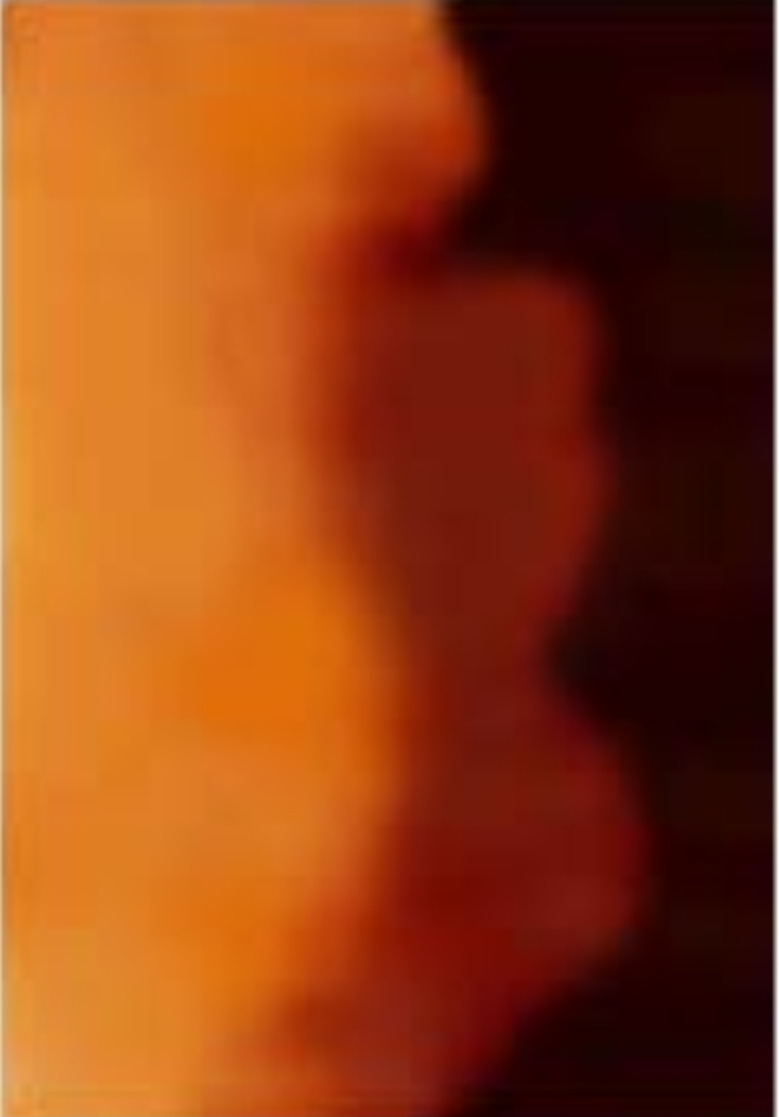
\includegraphics[width = 3.6cm]{Introduction/graphene.png}
\hspace{3cm}
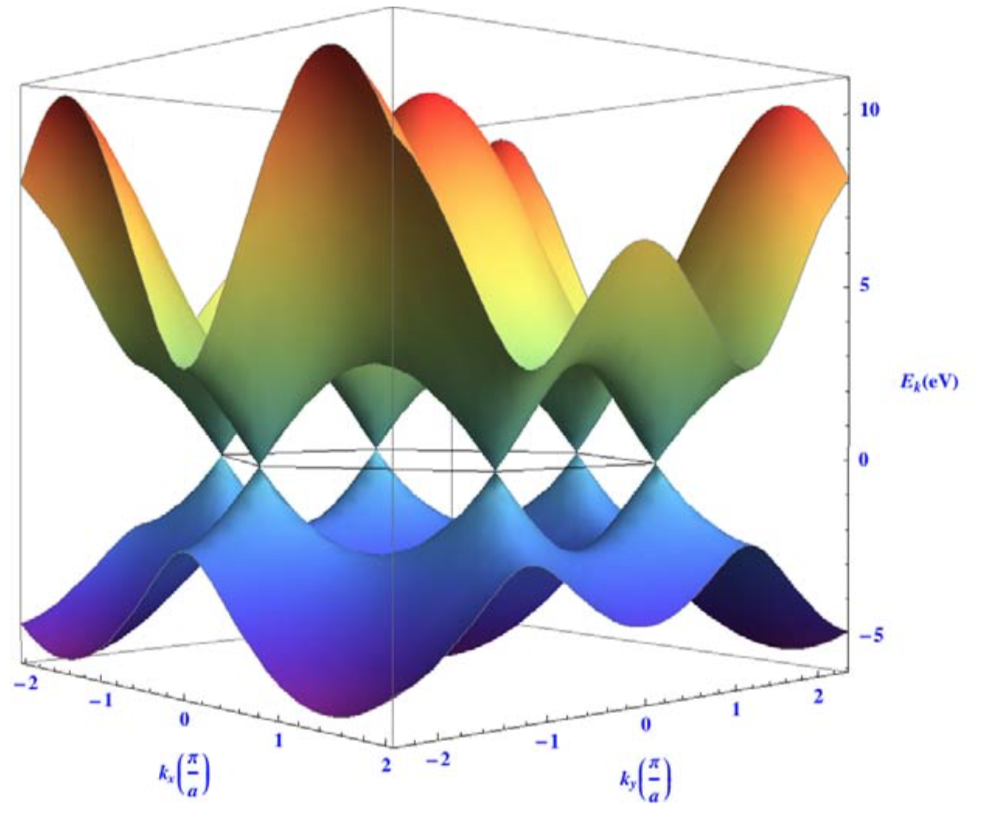
\includegraphics[width = 6.5cm]{Introduction/disp_rel.png}
\caption[Graphene monolayer; graphene's dispersion relation.]{Left: \acf{AFM} picture of a graphene monolayer. The black area is a substrate used for fabrication purposes. The dark orange area is a monolayer of graphene. Right: Dispersion relation of graphene. The black line represents the Fermi energy. Close to it, the dispersion relation is linear, corresponding to massless excitations (taken from \cite{noauthor_nobel_nodate}). }
\label{fig:graphene}
\end{figure}	

On the other hand, \acp{TMD} are a recent member of the \ac{2D} materials family \cite{wang_electronics_2012, roldan_electronic_2014, xu_spin_2014}.
\acp{TMD} have been attracting interest because they seem to overcome some of the drawbacks of graphene in technological applications.
For example, monolayer graphene is gapless, while its bilayer counterpart has only a tunable, but small gap of the order of a tenth of an $eV$.
Contrastingly, \acp{TMD} have an intrinsic gap in excess of $1 \, eV$, being more promising in designing, for example, transistors.
Hole-doped \acp{TMD} are expected to show topological superconductivity \cite{hsu_topological_2017}, while the superconducting phase of graphene has been predicted, but is not easily attained.
Superconductivity in graphene-like \ac{2D} materials is important because it could boost high speed nanoelectronics.
Moreover, the presence of transition metal atoms in \acp{TMD} suggests the possibility of magnetic ordering \cite{braz_valley_2017}, which could be very relevant in nanospintronics applications.
Both topological superconductivity and magnetic ordering arise due to the effect of strong electron correlations.
Thus, to investigate these properties of \acp{TMD} when performing simulations, we need a computational method that is robust enough to capture the effects of electron interactions.

A nanoribbon consists of a \ac{2D} layer that can be regarded as infinitely long on one direction, but not on the other (Figure \ref{fig:fabrication}), so that edge states become relevant, and can be controlled to yield interesting properties.
For simulation purposes, it is natural to assume translational invariance along the ribbon's longitudinal direction, and use \acp{PBC}.
On the other direction, we use \acp{OBC}, effectively considering zigzag edges (Figure \ref{fig:nanoribbons}, left).

\begin{figure}[H]
\centering
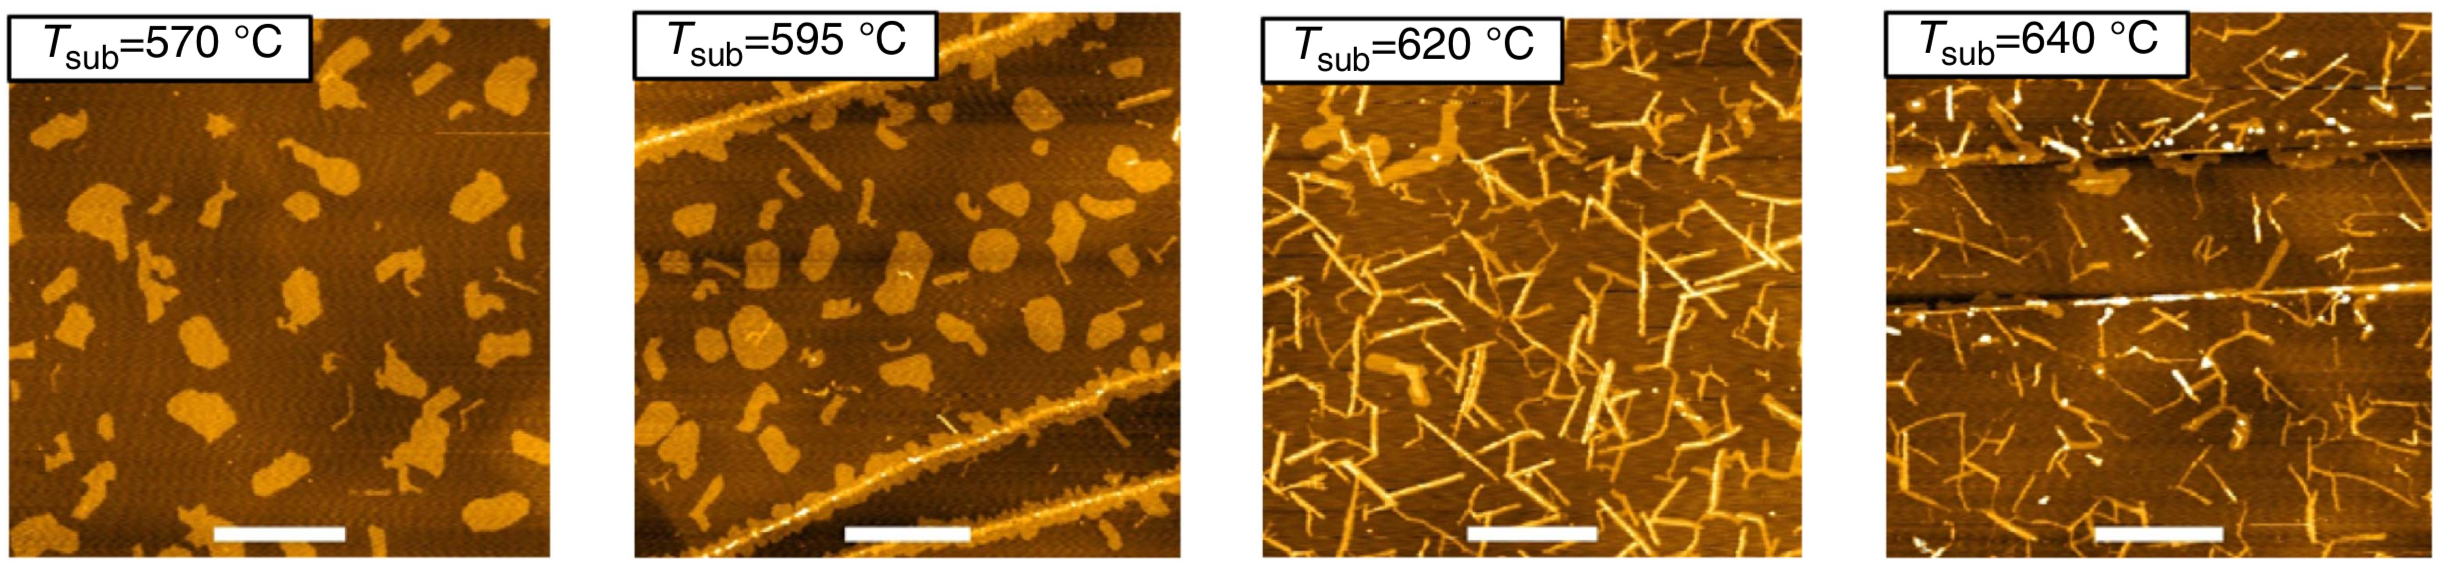
\includegraphics[scale = 0.35]{Introduction/nanoribbons}
\caption[Fabrication of \ac{TMD} nanoribbons]{Fabrication of \ac{TMD} nanoribbons. From left to right, we see \ac{AFM} images showing the appeareance of nanostructures ranging from \ac{2D} nanoislands to nanoribbons, as the temperature of the substrate is increased. The nanoribbons are grown by taking advantage of the temperature dependence of shape transformations occuring during the nonequilibrium growth of this kind of surface-based nanostructures. (taken from \cite{chen_fabrication_2017})}
\label{fig:fabrication}
\end{figure}
   
A high density of low-energy electronic states is localized at the zigzag edges, decaying quickly in the bulk, which suggests the possibility of magnetic ordering.
In fact, a mean field solution of the Hubbard model for a graphene nanoribbon shows that magnetic moments are localized at the edges \cite{yazyev_emergence_2010} (Figure \ref{fig:nanoribbons}, right).
QMC has been used to investigate edge-state magnetism beyond mean field in graphene \cite{feldner_dynamical_2011, golor_quantum_2013, cheng_strain-induced_2015, raczkowski_interplay_2017, yang_strain-tuning_2017}.
However, edge magnetism in TMD nanoribbons remains unexplored \cite{davelou_nanoribbon_2017}.
 
\begin{figure}[H]
\hspace{2cm}
\begin{minipage}[c]{0.1\textwidth}
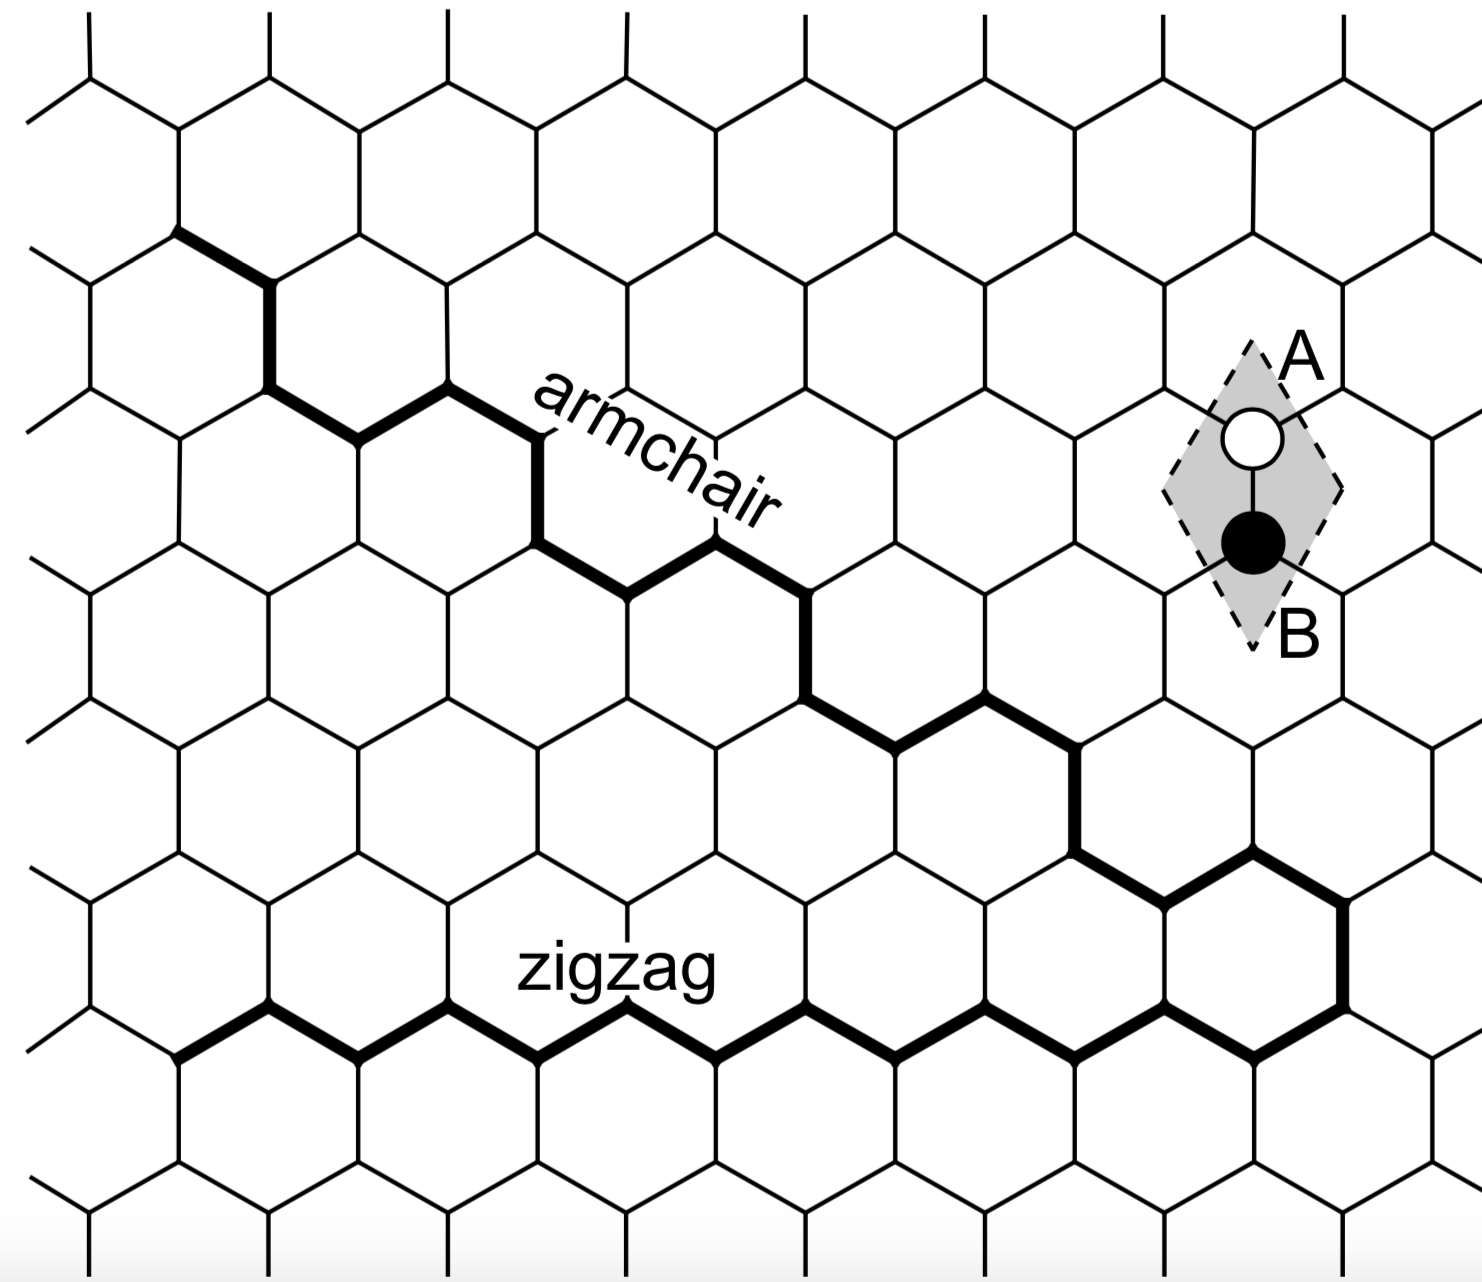
\includegraphics[scale = 0.22]{Introduction/zigzag}
\end{minipage} \hspace{6cm}
\begin{minipage}[c]{0.1\textwidth}
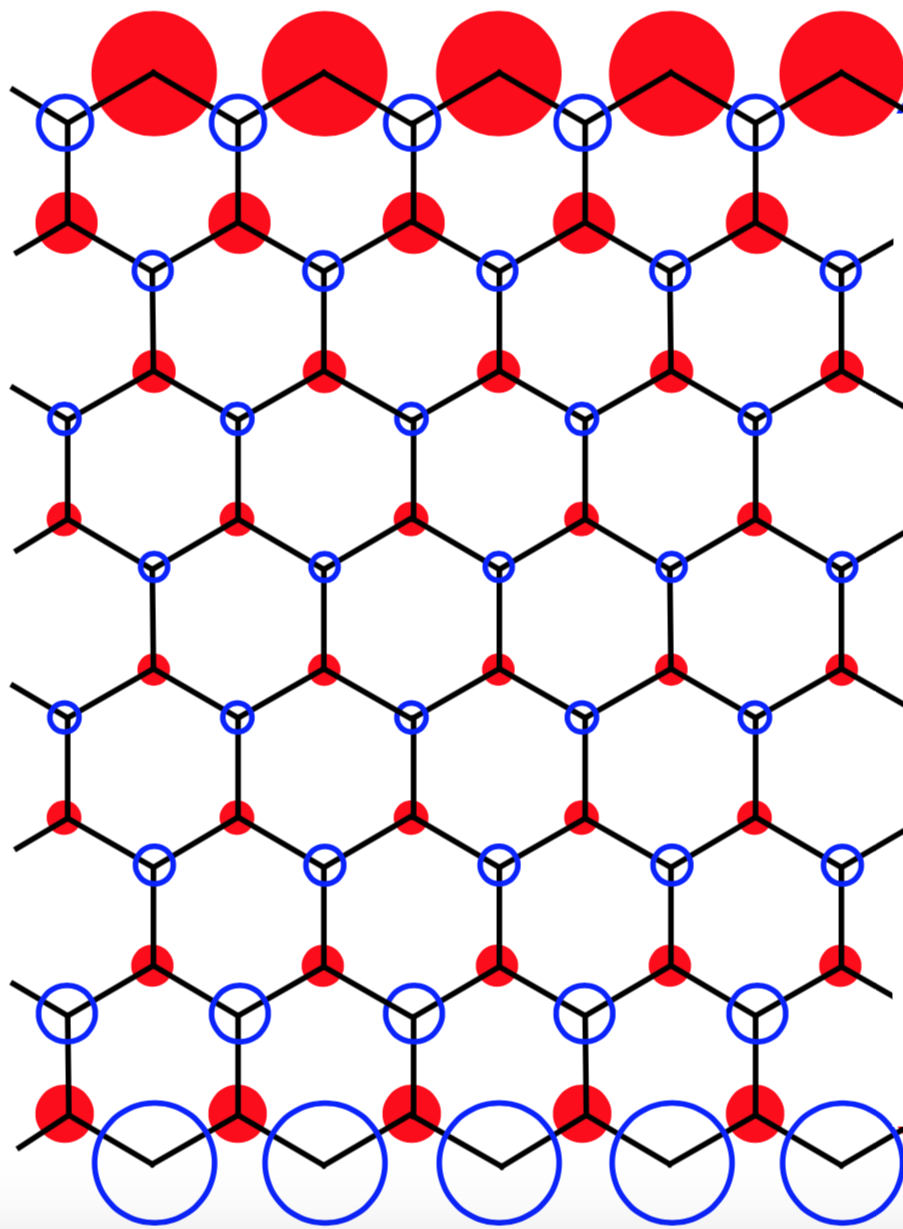
\includegraphics[scale = 0.23]{Introduction/edge_states}
\end{minipage}
 \caption[Zigzag edges of a nanoribbon and magnetism.]{Left: Two possible terminations of a \ac{TMD} nanoribbon condensing in a honeycomb lattice. Right: Local magnetic moments exist on the zig zag edges. The area of the circles corresponds to the magnitude of the magnetic moment, while the color red corresponds to a spin up density, and blue to a spin down density. The accumulation of electronic edge states leads to an \ac{AF} ground state (opposite edges with opposite magnetic moment). (taken from \cite{yazyev_emergence_2010}) \label{fig:nanoribbons}}
\end{figure}

While the zigzag graphene nanoribbon antiferromagnetic ground state is semiconducting, a state with interedge ferromagnetic orientation is a metal.
An example of an application based on the switching between the two states is a magnetorresistive sensor.
This device allows switching between low and high-resistance configurations, corresponding, respectively, to parallel, and antiparallel configurations of ferromagnetic leads at the ends of a nanoribbon.
An important application of this project is precisely the investigation of the possibility of edge-state magnetism, as is observed in graphene nanoribbons, for TMD nanoribbons, which could yield similarly innovative applications.


\subsection{Introduction to \acl{QMC}}

In principle, the properties of a quantum many-fermion system can all be deduced by solving an extremely complicated Schr\"odinger equation that takes into account the coupling of all (identical) particles of the system.
However, for the majority of systems the resulting integrals have no analytic solution, so we solve the problem by numerical integration.
But there is a myriad of methods to evaluate integrals numerically.
How do we pick the best one for this case? 
Multi-dimensional integrals are plagued by the curse of dimensionality.
Although the Newton-Cotes quadrature formulas (including, for example the Newton method, and Simpson's rules), Gaussian quadrature formulas, or Romberg's method all scale polynomially with the number of integration points, they become impractical as the dimension increases.
To use them, one would invoke Fubini's theorem to reduce the multi-dimensional integral to a series of one-dimensional integrals.
However, the number of function evaluations required to compute the whole integral grows exponentially with its dimension.
The Monte Carlo method preserves the polynomial scaling, thus yielding comparable accuracy with far less function evaluations.
It is natural to use it since typically the state space of our quantum system is huge, leading to high dimensional integrals.

The Monte Carlo method is ubiquitous.
Its central idea is to use randomness to produce accurate estimates of deterministic integrals.
The term was coined by Nicolas Metropolis in 1949, first appearing in a seminal paper, in which it was described as a \say{statistical approach to the study of differential equations, or more generally, of integro-differential equations that occur in various branches of sciences}\cite{metropolis_monte_1949}.
Although it was used as early as 1777 in an experiment known as Buffon's needle - where one obtains an estimate of the constant $\pi$ by repeatedly throwing a needle randomly onto a sheet of paper with evenly spaced lines - it was crucially developed in the Los Alamos National Laboratory during World War II where the development of the first atomic bomb was completed, the primary objective of the Manhattan Project.
The method is particularly useful when one wants to sample from a probability distribution in an exponentially large state space.
In fact, it can in principle be used to solve any problem allowing a probabilistic formulation.

A variety of \acf{QMC} methods exists, using a sampling scheme based on the Metropolis algorithm, and variations thereof.
Variational and Diffusion \ac{QMC} are the simplest \ac{QMC} methods that allow one to capture some properties of correlated systems.
Although they already contain the main concepts used in this type of simulations, it is not always possible to use them. 
We will discuss their flaws and show how further refinement leads to the determinant, or auxiliary field method we ultimately used.

Using the Monte Carlo approach to study a many-fermion system implies overcoming a significant obstacle common to all \ac{QMC} methods - the so called \emph{fermion-sign problem}.
Pauli's exclusion principle implies that the many-fermion wave function is anti-symmetric, which leads to a sign oscillation that greatly impedes the accurate evaluation of averages of quantum observables.
The anti-symmetry constraint implies that a  straightforward weight interpretation of the wave function is not possible.
In the case of the finite temperature algorithm, the cancellations that occur when computing the average of any physical observable lead to poor statistical properties of the corresponding estimators.
This means that a massive amount of samples requiring enormous computer time are needed to obtain meaningful results.
In the case of the zero temperature algorithms, the situation is even worse.
It might not even be possible to design a stochastic process carrying the system to its ground state, as normally is done in \say{projective} methods\footnote{Methods that iteratively project a trial wave function onto the ground state.}: the wave function that is used as an initial proposal turns out to converge to a bosonic one, and the fermionic character of the system is lost.

As was proven by Troyer, the \emph{fermion-sign problem} has NP\footnote{NP or nondeterministic polynomial time, meaning that one can devise an algorithm that verifies the "yes" answer to a decision problem in polynomial time in the system size.
Note that the class $P$ - of polynomial time algorithms - is a subclass of NP.} computational complexity \cite{troyer_computational_2005}.
One of the greatest open questions in computer science is whether $P = NP$.
Solving the \emph{fermion-sign problem} would imply finding a solution to $P = NP$, which would constitute a major breakthrough.



\subsection{Variational Monte Carlo}

Variational techniques rely on an educated guess for the wave function of the system.
One introduces a set of variational parameters $\bm \alpha$ that are then tuned according to a variational principle.
Then, we may use the optimized trial wave function to compute physical quantities of interest using Monte Carlo.
The method is used to obtain zero temperature properties of a given model.
Note that it requires prior knowledge about the system to propose an approximate wave function in the first place.

A particularly relevant observable is the variational energy $E_V$ associated to a trial ground state.
Let $\bm r$ be the $3N$ spatial coordinates of the $N$ electrons.
Given the Hamiltonian of the system $\mathcal{H}$, and a trial wave function $\psi (\bm r)$ - a guess of the wave function representing the ground state - one can compute the corresponding variational energy.

\begin{equation}\label{eq:variational_energy}
E_V = \frac{\left\langle \psi | \mathcal{H} | \psi \right \rangle}{\left\langle \psi | \psi \right \rangle} = \frac{ \int d\bm r |\psi (\bm r)|^2 E_L (\bm r)}{\int d\bm r | \psi (\bm r)|^2 } = \int d\bm r\rho (\bm r) E_L (\bm r) ,
\end{equation}
where the local energy $E_L (\bm r)$ is defined as

\begin{equation}\label{eq:local_energy}
E_L = \frac{\mathcal{H} \psi (\bm r) }{\psi (\bm r)}
\end{equation}
and the probability distribution $\rho (\bm r)$ is defined as

\begin{equation}\label{eq:rho}
\rho (\bm r) = \frac{ | \psi (\bm r) |^2}{ \int d\bm r' | \psi (\bm r') |^2}
\end{equation}

Note that we managed to recast the variational energy as an average of the \emph{local} energy, $\left\langle E_L \right\rangle $, over the the distribution $\rho$.
This may be computed using the Monte Carlo method by sampling $M$ points $\bm r_k$ from distribution $\rho (\bm r)$:

\begin{equation}\label{eq:average}
E_V \approx \overline{E}_L = \frac{1}{M} \sum_{k= 1}^{M} E_L (\bm r_k) ,
\end{equation}
where $\overline {X}$ denotes a sample mean of the random variable $X$.

Let the ground state energy be $E_0$.
Then, states are optimized according to the variational principle:

\begin{equation}
E_V(\bm \alpha) = \frac{\left\langle \psi_{\bm \alpha} | \mathcal{H} | \psi_{\bm \alpha} \right\rangle}{\left\langle\psi_{\bm \alpha} | \psi_{\bm \alpha} \right\rangle} \ge E_0,
\end{equation}
where $\psi_{\bm \alpha}$ is the trial ground state wave function for the set of variational parameters ${\bm \alpha}$.

By varying $\bm \alpha$ we aim to obtain a variational energy that is as close as possible to the true ground state energy.
Since $E_V(\bm \alpha)$ is bounded from below, this is equivalent to minimizing it in the hope that $E_V(\bm \alpha_{min}) \gtrsim E_0$, i.e. the bound is tight.

The finite sampling size $M$, of course, introduces a statistical error common to all Monte Carlo methods. 
However, the use of an approximate wave function introduces a systematic error that is hard to control since trial wave functions are generally introduced based on approximate, or heuristic arguments.

\subsection{Diffusion Monte Carlo and projective methods}\label{subsec:dmc}

Variational Monte Carlo is severely limited by the use of a trial wave function $\psi_{\bm \alpha} (\bm r)$ because we may even not have enough information to even construct a reliable variational wave function.

Diffusion \ac{QMC} allows the simulation of a many-body system while having only a limited knowledge of the system's physical properties.
While it is exact for many-boson systems, it is only approximate for many-fermion systems.
The idea is to map the Schr\"odinger equation into  an imaginary-time diffusion equation.
Excited states are then filtered out by a diffusion process as we advance in imaginary-time.
In imaginary-time $\tau = i t$, the solution to the Schr\"odinger equation in terms of a formal series expansion in the eigenfunctions of the hamiltonian becomes a series of transients $e^{-E_n \tau}, \, n \in \mathbb{N}$.
The longest lasting of these is the ground state  \cite{kosztin_introduction_1996}.

The idea of the diffusion method is to generate samples using the exact ground state wave function $\psi_0 (\bm r)$ \cite{toulouse_chapter_2016}.
The associated exact energy $E_0$ is the matrix element of the hamiltonian calculated using a trial wave function and the ground state wave function.

\begin{equation}
E_0 = \frac{ \left\langle \psi_0 |E_0 \mathbbm{1} | \psi \right\rangle}{\left\langle \psi_0 | \psi \right\rangle} = \frac{\left\langle \psi_0 | \mathcal{H} | \psi \right\rangle}{ \left\langle\psi_0 | \psi \right\rangle} = \frac{\int d\bm r \psi_0^\star (\bm r) \psi (\bm r) E_L (\bm r)}{\int d\bm r\psi_0^\star (\bm r) \psi (\bm r)}
\end{equation}

Note that using this trick we avoid the computation of $\mathcal{H} \psi_0 = E_0 \psi_0$, that is, the ground state energy.
Instead, we approximate the integral by considering $M$ configuration samples $\bm r_{k = 1,..., N}$ in a similar spirit to that of Variational \ac{QMC}.
Notice that the integral consists of a local energy of the trial wave function $E_L (\bm r) = \frac{\mathcal{H} \psi (\bm r)}{\psi (\bm r)}$ averaged over a mixed distribution from which we draw a sample of points $\bm r_{k=1,...M}$:

\begin{equation}
f(\bm r) = \frac{\psi_0^\star (\bm r) \psi (\bm r) }{ \int d\bm r  \psi_0 (\bm r) \psi (\bm r)}
\end{equation}

Although the method is, of course, aimed at probing many-body systems, let us consider a single particle in \acs{1D} for simplicity for illustrating the method.
Performing a Wick rotation - effectively going to imaginary time - and shifting the energy, the Schr\"odinger equation becomes

\begin{equation}
\frac{\partial \psi ( x, \tau )}{\partial\tau}  = -\frac{1}{2m}\frac{\partial^2 \psi ( x, \tau )}{\partial x^2} - \bigg[ V(x) - E_T \bigg] \psi( x, \tau ) 
\end{equation}

The exact ground state wave function $\psi_0 ( x )$ is obtained as the longest lasting transient state in imaginary time: we are interested in the asymptotic behavior of the series expansion constituting the formal solution of the Schr\"odinger equation

\begin{equation}
\psi (x, \tau) = \sum_{n=0}^{\infty} c_n \psi_n (x) e^{-(E_n - E_T)\tau}
\end{equation}

Imaginary time evolution is governed by

\begin{equation}\label{eq:im_ev}
\begin{split}
&\left| \psi (t) \right\rangle = \lim_{\tau \rightarrow \infty} \sum_i e^{-(E_i - E_T) \tau} \left|\psi_i \right\rangle \left\langle \psi_i | \psi \right\rangle = \\
&= \lim_{\tau \rightarrow \infty} e^{-(E_0 - E_T)\tau} \left| \psi_0 \right\rangle \left\langle \psi_0 | \psi \right\rangle 
\end{split}
\end{equation}


If $E_T > E_0$ the wave function diverges exponentially fast: $\lim_{\tau \rightarrow \infty} \psi ( x, \tau) = \infty$.
Similarly, for $E_T < E_0$ it vanishes exponentially fast: $\lim_{\tau \rightarrow \infty} \psi ( x, \tau) = 0$.
However, if $E_T = E_0$ the wave function converges to the ground state one up to a constant factor.

\begin{equation}\label{eq:dmc}
\lim_{\tau \rightarrow \infty} \psi ( x, \tau) = c_0 \psi_0 (x) \,\,\, \text{, or} \quad \lim_{\tau \rightarrow \infty} \left|\psi (\tau) \right\rangle \propto \left| \psi_0 \right\rangle
\end{equation}

Diffusion \ac{QMC} makes use of Eq. (\ref{eq:dmc}), approximating $\psi_0(x)$ by $\psi (x, \tau)$ for sufficiently long time.
The only requirement is that $\psi (x, \tau)$ and $\psi_0(x)$ overlap significantly so that $c_0$ is large enough to be numerically measurable, and we can always center a positive trial wave function in a region where $\psi_0(x)$ is large enough and positive.
If the latter condition does not hold, the wave function converges to a bosonic, instead of a fermionic one.
Of course, these conditions can always be met for a single particle, but note that they might fail for a many-fermion system, for which the wave function crosses a number of nodes due to its anti-symmetric nature.

\subsection{Drawbacks of variational and projective methods. Auxiliary Field \acs{QMC}. The Fermion Sign Problem.}
\label{subsec:introAFQMC}

As we have seen, the major drawback of the variational method was that it demanded \emph{a priori} knowledge of a reasonable variational wave function describing, at least partly, some of the physics of the problem.
Diffusion \acs{QMC} demands less: we need only propose a trial wave function that overlaps with the ground state.
However, none of these methods allow us to probe systems at finite temperature.
Moreover, they both require some prior knowledge about the system, which may not always be available.

An alternative method is based on introducing an additional lattice bosonic field that mediates the electron-electron interaction.
The interacting problem then becomes a problem of independent fermions coupled to an external field, and the fermionic part of the partition function can be traced out explicitly, leaving the contribution of a \emph{discrete}\footnote{Although, there is a finite number of field configurations, the number grows exponentially with the number of sites on the lattice.} bosonic field.
This contribution can be evaluated numerically by employing importance sampling over the field configurations.
Auxiliary field \acs{QMC} relies on a mapping to a classical system:

\begin{equation}
Z = \Tr [ e^{-\beta \mathcal{H} } ] = \sum_c p_c ,
\end{equation}
but some of the \say{probabilities} can actually be negative $p_c < 0$.
This occurs due to the antisymmetry of the many-electron wave function under exchange of two electrons.

The negative weight problem may easily be circumvented when computing averages of observables:

\begin{equation}\label{eq:signSampling}
\left\langle A \right\rangle = \frac{\sum_c A ( c ) p ( c )}{\sum_c p ( c ) } = \frac{\sum_c A ( c )|  p ( c ) | \text{sign}[p(c)] / \sum_c | p ( c ) | }{\sum_c  |  p ( c ) | \text{sign}[p(c)] /  \sum_c | p ( c ) |} \equiv \frac{\left\langle A s \right\rangle_{|p|}}{\left\langle s \right\rangle_{|p|}} ,
\end{equation}
where $s(c) = \text{sign} [ p ( c ) ]$, and $| p ( c ) | $ corresponds to an auxiliary bosonic system (also coupled to the bosonic field) corresponding to the original fermionic system, and for which there is no sign problem.

The relative error $\Delta s / \left\langle s \right\rangle$ increases exponentially with the number of particles, with inverse temperature, and possibly with other parameters of the specific model to be studied \cite{troyer_computational_2005, hou_numerical_2009}.
To see this, we start by noting that the average sign is the ratio between the partition functions of the fermionic ($Z = \sum_c p(c)$) and bosonic systems ($Z = \sum_c | p ( c ) |$).
In terms of the difference in free energy densities, $\left\langle s \right\rangle = Z / Z' = e^{-\beta N_p \Delta f}$, implying that for $M$ samples, the error of the denominator of Eq. (\ref{eq:signSampling}) becomes

\begin{equation}
\frac{\Delta s}{\left\langle s \right\rangle} = \frac{\sqrt{(\left\langle s^2 \right\rangle - \left\langle s \right\rangle^2 )/ M }}{\left\langle s \right\rangle} = \frac{ \sqrt{ 1 - \left\langle s \right\rangle^2}  }{\sqrt{M} \left\langle s \right\rangle} \propto \frac{e^{\beta N_p \Delta f}}{\sqrt{M}} ,
\end{equation}
and similarly for the numerator of Eq. (\ref{eq:signSampling}).

Auxiliary field \acs{QMC} can also be formulated to probe ground state properties, and a sign problem arises similarly.
Apart from this problem, which plagues all \acs{QMC} methods, this method is one of the most robust, unbiased, and reliable methods, hence we choose it to carry out our simulations.
Note that, in particular, it is certainly more powerful than the variational and diffusion methods outlined before since it requires much less \emph{a priori} information about the system.
Perhaps more importantly, given some recent findings, it can be used in conjunction with neural networks to discover quantum phase transitions in correlated systems  \cite{broecker_machine_2017}.
\section{Introduction to \acl{QMC}}
\label{sec:introQMC}

Solving the many-body problem remains one of the greatest challenges in physics.
Following the wealth of attempts at such pursuit, certain phenomena arising due to the strong interactions in quantum systems are explained in different theoretical frameworks, namely superconductivity, the Mott metal-insulator transition, and fractional quantum Hall effect.
All of these breakthroughs represented revolutions in their respective fields with significant scientific and technological impact.
However, only in very limited cases does an actual analytical solution exist for the  Schr\"odinger equation for a system of interacting particles.
One must resort to sophisticated approximation methods to obtain  information about the role played by the competing interactions under various conditions in the aforementioned cases.
It is then natural that numerical methods have become prominent as a tool for extracting useful information about this type of systems.
\ac{QMC} is amongst the most accurate and extensively studied ones.
The idea of all \ac{QMC} methods is to reduce the interacting problem to solving a set of integrals, which can be evaluated numerically through a standard stochastic procedure.
These integrals are arrived at upon formulating the quantum many-body description of the system using the Schr\"odinger equation.
Hence the name \acl{QMC}, which is used to distinguish it from Classical Monte Carlo.
In the classical version, one measures thermal averages, while in the quantum version, one measures expectations of operators over the Hilbert space of the system, corresponding to physical observables that fluctuate with a dynamics given by the Schr\"odinger equation (and, of course, can also have thermal fluctuations).
In fact, the dynamics of a quantum system are encoded in the Hamiltonian operator.
In the case of graphene-like \ac{2D} materials, one usually uses a tight-binding model.
It is found that the dynamics given by the tight-binding Hamiltonian is sufficient to describe most properties of graphene.
However, in other materials, such as \acp{TMD}, electron-electron interactions are stronger, and Hubbard-type models could give us a more accurate picture of the phenomena that occur within them.

For quantum many-fermion systems, observables are given in terms of integrals which have no analytic solution, so we solve the problem numerically.
But there is a myriad of methods to evaluate integrals numerically.
How do we pick the best one for this case? 
Multi-dimensional integrals are plagued by the curse of dimensionality.
Although the Newton-Cotes quadrature formulas (including, for example the Newton method, and Simpson's rules), Gaussian quadrature formulas, or Romberg's method all scale polynomially with the number of integration points, they become impractical as the dimension increases.
To use them, one would invoke Fubini's theorem to reduce the multi-dimensional integral to a series of one-dimensional integrals.
However, the number of function evaluations required to compute the whole integral grows exponentially with its dimension.
The Monte Carlo method preserves the polynomial scaling, thus yielding comparable accuracy with far less function evaluations.
It is natural to use it since typically the state space of our quantum system is huge, leading to high dimensional integrals.

The Monte Carlo method is ubiquitous.
Its central idea is to use randomness to produce accurate estimates of deterministic integrals.
The term was coined by Metropolis in 1949, although it was used as early as 1777 in an experiment known as Buffon's needle - where one obtains an estimate of the constant $\pi$ by repeatedly throwing a needle randomly onto a sheet of paper with evenly spaced lines. %t was crucially developed in the Los Alamos National Laboratory during World War II where the development of the first atomic bomb was completed, the primary objective of the Manhattan Project.
The method is particularly useful when one wants to sample from a probability distribution in an exponentially large state space (like the huge Hilbert space of an interacting electron system), but it can, in principle, be used to solve any problem allowing a probabilistic formulation.
To solve the interacting fermion problem, a variety of \ac{QMC} methods exists, using a sampling scheme based on the Metropolis algorithm, and variations thereof.
Variational and Diffusion \ac{QMC} are the simplest \ac{QMC} methods that allow one to capture some properties of correlated systems, but it is not always ideal or even possible to use them. 
%We will discuss their flaws and show how further refinement leads to the auxiliary field method we ultimately used.

Using the Monte Carlo approach to study a many-fermion system implies overcoming a significant obstacle common to all \ac{QMC} methods - the so called \emph{fermion sign problem}.
Pauli's exclusion principle implies that the many-fermion wave function is anti-symmetric, which leads to a sign oscillation that greatly impedes the accurate evaluation of averages of quantum observables.
The anti-symmetry constraint implies that a  straightforward weight interpretation of the wave function is not possible.
In the case of the finite temperature algorithm, the cancellations that occur when computing the average of any physical observable lead to poor statistical properties of the corresponding estimators.
This means that a massive amount of samples requiring enormous computer time are needed to obtain meaningful results.
In the case of the zero temperature algorithms, the situation is even worse.
It might not even be possible to design a stochastic process carrying the system to its ground state, as normally is done in \say{projective} methods\footnote{Methods that iteratively project a trial wave function onto the ground state.}: the wave function that is used as an initial proposal turns out to converge to a bosonic one, and the fermionic character of the system is lost.
As was proven by Troyer, the \emph{fermion sign problem} has NP\footnote{NP or nondeterministic polynomial time, meaning that one can devise an algorithm that verifies the "yes" answer to a decision problem in polynomial time in the system size.
Note that the class $P$ - of polynomial time algorithms - is a subclass of NP.} computational complexity \cite{troyer_computational_2005}.
One of the greatest open questions in computer science is whether $P = NP$.
Solving the \emph{fermion sign problem} would imply finding a solution to $P = NP$, which would constitute a major breakthrough.

\subsection{Variational Monte Carlo}

Variational techniques rely on an educated guess for the wave function of the system.
One introduces a set of variational parameters $\bm \alpha$ that are then tuned according to a variational principle.
Then, we may use the optimized trial wave function to compute physical quantities of interest using Monte Carlo.
The method is used to obtain zero temperature properties of a given model.
Note that it requires prior knowledge about the system to propose an approximate wave function in the first place.

A particularly relevant observable is the variational energy $E_V$ associated to a trial ground state.
Let $\bm r$ be the $3N$ spatial coordinates of the $N$ electrons.
For simplicity, let us ignore all other degrees of freedom, such as spin.
Given the Hamiltonian of the system $\mathcal{H}$, and a trial wave function $\psi_T (\bm r)$ - a guess of the wave function representing the ground state - one can compute the corresponding variational energy by averaging over a \say{local} energy:

\begin{equation}\label{eq:variational_energy}
E_V = \frac{\left\langle \psi_T | \mathcal{H} | \psi_T \right \rangle}{\left\langle \psi_T | \psi_T \right \rangle} = \frac{ \int d\bm r |\psi_T (\bm r)|^2 E_L (\bm r)}{\int d\bm r | \psi_T (\bm r)|^2 } = \int d\bm r\rho (\bm r) E_L (\bm r) , \text{where}
\end{equation}

\begin{equation}\label{eq:local_energy}
E_L = \frac{\mathcal{H} \psi_T (\bm r) }{\psi_T (\bm r)}   \quad \text{and} \quad \rho (\bm r) = \frac{ | \psi_T (\bm r) |^2}{ \int d\bm r' | \psi_T (\bm r') |^2}
\end{equation}

Note that we managed to recast the variational energy as an average of the \emph{local} energy, $\left\langle E_L \right\rangle $, over the the distribution $\rho$.
This may be computed using the Monte Carlo method by sampling $M$ points $\bm r_k$ from the distribution $\rho (\bm r)$.
Denoting the sample mean of the random variable $X$ as $\overline {X}$:

\begin{equation}\label{eq:average}
E_V \approx \overline{E}_L = \frac{1}{M} \sum_{k= 1}^{M} E_L (\bm r_k) ,
\end{equation}

Let the ground state energy be $E_0$.
Then, states are optimized according to the variational principle:

\begin{equation}
E_V(\bm \alpha) = \frac{\left\langle \psi_{\bm \alpha} | \mathcal{H} | \psi_{\bm \alpha} \right\rangle}{\left\langle\psi_{\bm \alpha} | \psi_{\bm \alpha} \right\rangle} \ge E_0,
\end{equation}
where $\psi_{\bm \alpha}$ is the trial ground state wave function for the set of variational parameters ${\bm \alpha}$.
By varying $\bm \alpha$ we aim to obtain a variational energy that is as close as possible to the true ground state energy, and use the corresponding trial wave function to compute averages of other observables.
Since $E_V(\bm \alpha)$ is bounded from below, this is equivalent to minimizing it in the hope that $E_V(\bm \alpha_{min}) \gtrsim E_0$, i.e. the bound is tight.
The finite sampling size $M$, of course, introduces a statistical error common to all Monte Carlo methods. 
However, the use of an approximate wave function introduces a systematic error that is hard to control since trial wave functions are generally introduced based on approximate, or heuristic arguments.

\subsection{Diffusion Monte Carlo and projective methods}\label{subsec:dmc}

Variational Monte Carlo is severely limited by the use of a trial wave function $\psi_T (\bm r)$ because we may not even have enough information to even construct a reliable variational wave function in the first place.
Diffusion \ac{QMC} allows the simulation of a many-body system while having only a limited knowledge of the system's physical properties.
As a projective method, it is exact for many-boson systems, while being only approximate for many-fermion systems.
The idea is to map the Schr\"odinger equation onto an imaginary-time diffusion equation.
Excited states are then filtered out by a diffusion process as we advance in imaginary-time.
In imaginary-time $\tau = i t$, the solution to the Schr\"odinger equation in terms of a formal series expansion in the eigenfunctions of the Hamiltonian becomes a series of \say{transient} wavefunctions weighted by $e^{-E_n \tau}, \, n \in \mathbb{N}$.
Within precision and accuracy constraints, the longest lasting of these is the ground state \cite{kosztin_introduction_1996}.
Thus, the idea of the diffusion method is to generate samples using the exact ground state wave function $\psi_0 (\bm r)$ \cite{toulouse_chapter_2016}.
The associated exact energy $E_0$ is the matrix element of the hamiltonian calculated using a trial wave function and the ground state.

\begin{equation}
E_0 = \frac{ \big( \left\langle \psi_0 |E_0 \big) \big( \mathbbm{1} | \psi_T \right\rangle \big)}{\left\langle \psi_0 | \psi_T \right\rangle} = \frac{\left\langle \psi_0 | \mathcal{H} | \psi_T \right\rangle}{ \left\langle\psi_0 | \psi_T \right\rangle} = \frac{\int d\bm r \psi_0^\star (\bm r) \psi_T (\bm r) E_L (\bm r)}{\int d\bm r\psi_0^\star (\bm r) \psi_T (\bm r)}
\end{equation}

Note that using this trick we avoid the computation of $\mathcal{H} \psi_0 = E_0 \psi_0$, that is, the ground state energy.
Instead, we approximate the integral by considering $M$ configuration samples $\bm r_{k = 1,..., M}$ in a similar spirit to that of Variational \ac{QMC}.
Notice that the integral consists of a local energy of the trial wave function $E_L (\bm r) = \frac{\mathcal{H} \psi (\bm r)}{\psi (\bm r)}$ averaged over a mixed distribution from which we draw a sample:

\begin{equation}
f(\bm r) = \frac{\psi_0^\star (\bm r) \psi_T (\bm r) }{ \int d\bm r  \psi_0 (\bm r) \psi_T (\bm r)}
\end{equation}

Although the method is, of course, aimed at probing many-body systems, let us consider a single particle in \acs{1D}, for simplicity, to illustrate the method.
Performing a Wick rotation - effectively going to imaginary time - and shifting the energy, the Schr\"odinger equation becomes (with $\hbar = 1$)

\begin{equation}
\frac{\partial \psi_T ( x, \tau )}{\partial\tau}  = -\frac{1}{2m}\frac{\partial^2 \psi_T ( x, \tau )}{\partial x^2} - \bigg[ V(x) - E_T \bigg] \psi_T( x, \tau ) 
\end{equation}

The exact ground state wave function $\psi_0 ( x )$ is obtained as the longest lasting transient state in imaginary time: we are interested in the asymptotic behavior of the series expansion constituting the formal solution of the Schr\"odinger equation

\begin{equation}
\psi_T (x, \tau) = \sum_{n=0}^{\infty} c_n \psi_n (x) e^{-(E_n - E_T)\tau}
\end{equation}

Imaginary time evolution is governed by

\begin{equation}\label{eq:im_ev}
\left| \psi_T (t) \right\rangle = \lim_{\tau \rightarrow \infty} \sum_n e^{-(E_n - E_T) \tau} \left|\psi_n \right\rangle \left\langle \psi_n | \psi_T \right\rangle = \lim_{\tau \rightarrow \infty} e^{-(E_0 - E_T)\tau} \left| \psi_0 \right\rangle \left\langle \psi_0 | \psi_T \right\rangle 
\end{equation}

If $E_T > E_0$ the wave function diverges exponentially fast: $\lim_{\tau \rightarrow \infty} \psi_T ( x, \tau) = \infty$.
Similarly, for $E_T < E_0$ it vanishes exponentially fast: $\lim_{\tau \rightarrow \infty} \psi_T ( x, \tau) = 0$.
However, if $E_T = E_0$ the wave function converges to the ground state one up to a constant factor, $c_0 = \left\langle \psi_0 | \psi_T \right\rangle$.

\begin{equation}\label{eq:dmc}
\lim_{\tau \rightarrow \infty} \psi_T ( x, \tau) = c_0 \psi_0 (x) \quad \text{or} \quad \lim_{\tau \rightarrow \infty} \left|\psi_T (\tau) \right\rangle \propto \left| \psi_0 \right\rangle
\end{equation}

Diffusion \ac{QMC} makes use of Eq. (\ref{eq:dmc}), approximating $\psi_0(x)$ by $\psi_T (x, \tau)$ for sufficiently long time.
The only requirement is that $\psi_T (x, \tau)$ and $\psi_0(x)$ overlap significantly so that $c_0$ is large enough to be numerically measurable, and we can always center a positive trial wave function in a region where $\psi_0(x)$ is large enough and positive.
If the latter condition does not hold, the wave function converges to a bosonic, instead of a fermionic one.
Of course, these conditions can always be met for a single particle, but note that they might fail for a many-fermion system, for which the wave function crosses a number of nodes due to its anti-symmetric nature.

\subsection{Auxiliary Field \acs{QMC} and the Fermion Sign Problem}
\label{subsec:introAFQMC}

As we have seen, the major drawback of the variational method was that it demanded \emph{a priori} knowledge of a reasonable variational wave function describing, at least partly, some of the physics of the problem.
Diffusion \acs{QMC} demands less: we need only propose a trial wave function that overlaps with the ground state.
However, none of these methods allow us to probe systems at finite temperature.
Moreover, they both require some prior knowledge about the system, which may not always be available.

An alternative method is based on introducing an additional lattice bosonic field that mediates the electron-electron interaction.
The interacting problem then becomes a problem of independent fermions coupled to an external field, and the fermionic part of the partition function can be traced out explicitly, leaving the contribution of a \emph{discrete}\footnote{The introduced field is discrete (and \emph{binary}) because each fermionic state can only have occupations $n = 0, 1$. Although, there is a finite number of field configurations, the number grows exponentially with the number of sites on the lattice.} bosonic field, $\bm h$.
This contribution can be evaluated numerically by employing importance sampling over the field configurations.
Auxiliary field \acs{QMC} relies on a mapping to a so called \say{classical} system (in quotes because there may be no actual classical analogue):

\begin{equation}\label{eq:Zsign}
Z = \Tr [ e^{-\beta \mathcal{H} } ] = \sum_{\{ \bm h\} } \sum_{\text{fermionic}} e^{-S} = \sum_c p_c ,
\end{equation}
but some of the \say{probabilities} can actually be negative $p_c < 0$.
This occurs due to the antisymmetry of the many-electron wavefunction under electron exchange, and is at the root of the sign problem.
Here, $S$ is a fermion-boson action that we shall write out explicitly later.
For a fixed configuration of the bosonic field, we sum over the fermionic part exactly to obtain the weight of each configuration $p_c$.
The sum over $\bm h$ is carried out stochastically.

The negative weight problem may easily be circumvented when computing averages of observables:

\begin{equation}\label{eq:signSampling}
\left\langle A \right\rangle = \frac{\sum_c A ( c ) p ( c )}{\sum_c p ( c ) } = \frac{\sum_c A ( c )|  p ( c ) | \text{sign}[p(c)] / \sum_c | p ( c ) | }{\sum_c  |  p ( c ) | \text{sign}[p(c)] /  \sum_c | p ( c ) |} \equiv \frac{\left\langle A s \right\rangle_{|p|}}{\left\langle s \right\rangle_{|p|}} ,
\end{equation}
where $s(c) = \text{sign} [ p ( c ) ]$, and $| p ( c ) | $ corresponds to an auxiliary bosonic system (also coupled to the bosonic field) corresponding to the original fermionic system, and for which there is no sign problem.

The relative error $\Delta s / \left\langle s \right\rangle$ increases exponentially with the number of particles, with inverse temperature, and possibly with other parameters of the specific model to be studied \cite{troyer_computational_2005, hou_numerical_2009}.
To see this, we start by noting that the average sign is the ratio between the partition functions of the fermionic ($Z = \sum_c p(c)$) and bosonic systems ($Z' = \sum_c | p ( c ) |$).
In terms of the difference in free energy densities, $\left\langle s \right\rangle = Z / Z' = e^{-\beta N_p \Delta f}$, implying that for $M$ samples, the error of the denominator of Eq. (\ref{eq:signSampling}) becomes

\begin{equation}
\frac{\Delta s}{\left\langle s \right\rangle} = \frac{\sqrt{(\left\langle s^2 \right\rangle - \left\langle s \right\rangle^2 )/ M }}{\left\langle s \right\rangle} = \frac{ \sqrt{ 1 - \left\langle s \right\rangle^2}  }{\sqrt{M} \left\langle s \right\rangle} \propto \frac{e^{\beta N_p \Delta f}}{\sqrt{M}} ,
\end{equation}
and similarly for the numerator of Eq. (\ref{eq:signSampling}).

Auxiliary field, or determinant \acs{QMC} can also be formulated to probe ground state properties, and a sign problem arises similarly.
In fact, this problem plagues all \acs{QMC} methods, even though we showed it only for the determinant method\footnote{So called because, as we shall show later, $p_c$ boils down to a product of determinants that depends on the energy scales of the problem.}.
The latter is the most robust, unbiased, and reliable method, with a generally modest sign problem, hence we choose it to carry out our simulations.

Furthermore, in general, it suffices to use the finite temperature auxiliary field  method with $\beta$ large enough to probe ground state properties (for example, this is shown numerically for the Hubbard model on the square lattice in \cite{white_numerical_1989}).
In this case, the inverse temperature may be regarded as being analogous to a  projective parameter $\Theta$, characterizing convergence to the ground state, within statistical uncertainty.
Projector \ac{QMC}, the zero temperature version of auxiliary field \ac{QMC} is based on an equation similar to Eq.(\ref{eq:dmc}).
Any observable $A$ is computed by use of a trial wave function with some overlap with the ground state $\left\langle \psi_T | \psi_0 \right\rangle \neq 0$ (see \cite{f._assaad_quantum_2002} for more details on the projector method; in this work we focus on the finite temperature version since it is more general):

\begin{equation}
\left\langle A \right\rangle = \lim_{\Theta \rightarrow \infty} \frac{\left\langle \psi_T | e^{-\Theta \mathcal{H} } A e^{-\Theta \mathcal{H} } | \psi_T \right\rangle }{\left\langle \psi_T | e^{- 2 \Theta \mathcal{H} } | \psi_T \right\rangle}
\end{equation}

Note that auxiliary field \ac{QMC} is more powerful than the variational and diffusion methods outlined before since it requires much less \emph{a priori} information about the system.
Perhaps more importantly, recent work suggests that it can be used in conjunction with neural networks to discover quantum phase transitions in correlated systems  \cite{broecker_machine_2017} in what could be a revolution in the field.
\section{Original Contributions}
\label{sec:int_contributions}

In this work we focus mainly on the study of the magnetic properties of \ac{TMD} nanoribbons.
We compare our \ac{QMC} results with those obtained in the mean field approximation and benchmark them  against existing, \say{tried and true}  implementations (namely \texttt{ALF} \cite{bercx_alf_2017} and \texttt{QUEST} \cite{noauthor_quest_2012}), and early seminal studies \cite{hirsch_discrete_1983,white_numerical_1989}.

To carry out this study, we use \texttt{QUEST} and our own original implementation of the auxiliary field \ac{QMC} algorithm in \texttt{C++}.
The code we wrote can be used to simulate low-dimensional Hubbard-like models with different geometries to extend this work.
Additionaly, using our code, we characterize and compare different options to stabilize the matrix products needed to perform the simulations.
Lastly, we give a contribution to circumvent the fermion sign problem in an attempt to extract the maximum amount of information out of the Monte Carlo measurements.
\section{Outline}
\label{sec:int_outline}

We started this introductory chapter with the concept of emergence in strongly correlated electron systems.
Then, we proceeded to discuss the particular example we study in this thesis: the \acs{2D} \acs{TMD} nanoribbon.
In this system, we show that electron correlations give rise to emergent edge-state magnetism, which was unexplored numerically  before this work.
To tackle this interacting fermion system, we resort to a state-of-the-art determinant  \ac{QMC} algorithm.

In chapter (\ref{cap:hubbard}), we introduce the Hubbard model, a ubiquitous model of electron correlations.
We discuss analytical solutions of simple limiting cases, outline some approximation methods, and introduce Green's functions, which turn out to be the main object of our simulations.
Moreover, we formulate the mean field theory of the Hubbard model.
Then, we proceed to the simulation method.
In chapter (\ref{cap:afqmc}), we start by summarizing the main ideas about how to apply the Monte Carlo method to statistical physics problems.
In this context, we use original results of our simulations to illustrate the concepts in the specific context of our problem.
Still in chapter (\ref{cap:afqmc}), we introduce the auxiliary field method, and its various challenges, namely low temperature, and large size stabilization.

In chapter (\ref{cap:applications}), we apply the code we implemented for a variety of systems, benchmarking our code, and carrying out some original calculations both at the mean field level and using \acs{QMC} for \acp{TMD}.
Finally, in chapter (\ref{cap:conclusions}), we conclude by discussing the results obtained in the previous chapter in the context of the literature, and propose future work to be done on the topic.

\cleardoublepage

\fancychapter{Introduction}
\label{cap:int}

\slshape

The isolation of graphene in 2004 has led to a growing interest of the scientific community in \ac{2D} materials revealing extraordinary properties.
Among them are \acp{TMD}, appearing in the form of a variety of nanostructures.
Unlike in graphene, where electron interactions are relatively weak, in \acp{TMD}, electrons are strongly correlated, and one cannot overlook the interactions between them.
Analytical approaches to the solution of the problem are either hopeless, or rely on possibly unrealistic approximations.
In fact, the increased complexity of the models describing such highly correlated  materials, compared to their graphene counterparts, calls for sophisticated computer simulation methods, most notably \ac{QMC}.
In this introductory chapter, we start by  reviewing the literature on the physics of \acp{TMD}, focusing on their basic properties.
Then, we present a survey of simulation methods belonging to the \acl{QMC} class.
We introduce some basic concepts, and motivate the choice of the particular used  method.
Finally, we summarize our original contributions, and outline the structure of the thesis.

\normalfont

\section{Motivation}
\label{sec:motivation}

It might seem surprising that \ac{2D} systems were not considered as a real possibility before the discovery of graphene since they are often idealized in thought experiments, for example when investigating toy models of more complex higher dimensional systems.
In fact, while thin film deposition on comparably thicker substrates was commonplace long before 2004, \ac{2D} layers were thought not to exist independently from their 3D base.
Their existence was not expected \emph{a priori} because at first sight they seem to violate the Mermin-Wagner-Hohenberg theorem \cite{mermin_absence_1966, coleman_there_1973, hohenberg_existence_1967}, a no-go theorem that forbids ordering below three dimensions at finite temperature\footnote{\ac{2D} materials can be stable because not all the conditions of Mermin-Wagner-Hohenberg theorem are verified, namely the condition of short-ranged interactions. In the particular case of graphene sheets, ripples appear, which implies that the material is not strictly \ac{2D}, and thus can be stabilized. The issue is subtle, and is beyond the scope of this work.}.
The discovery of graphene paved the way for the search for similarly stable \ac{2D} materials, and since it was isolated, a plethora of these has been discovered.
A vast set of open problems remains to be solved within the realm of the fascinating and counterintuitive properties of the now huge variety of existing \ac{2D} systems.
In particular, in some of these, the effect of electron interactions is non negligible, leading to emergent phenomena.
These are collective effects that emerge as a result of the interactions between the individual components of a system.
The properties of the system's components do not directly percolate up; instead, they shape the interactions that dictate the system's properties sometimes in rather unexpected ways, leading to unusual behavior.

Interacting electron systems are often tackled by carrying out computer simulations.
\ac{QMC} is a family of numerical methods that are  amply applicable to condensed matter physics problems, and that are particularly well suited to study strongly correlated electrons.
Despite the system size being constrained due to limited simulation time, reliable, accurate and unbiased solutions are provided to the otherwise intractable quantum many-body problem.
The class of \acs{QMC} algorithms that is used in this work was introduced in the 1980's in a series of seminal papers by Hirsch and \acl{BSS}\footnote{After whom the \ac{BSS} algorithm, on which we based the implementation used in this work, is named.} \cite{hirsch_discrete_1983, hirsch_monte_1982, blankenbecler_monte_1981, hirsch_two-dimensional_1985, hirsch_monte_1983, hirsch_stable_1988, hirsch_antiferromagnetism_1989}, but it saw a recent surge \cite{dumitrescu_superconductivity_2016, berg_monte_2018, beyl_revisiting_2018, chang_recent_2015, esterlis_breakdown_2018, mondaini_determinant_2012, meng_characterization_2014, kung_characterizing_2016, johnston_determinant_2013, rademaker_determinant_2013, ying_determinant_2014, scalettar_numerical_2007, zhou_quantum_2014} due to the increase in computational power, and algorithmic development.
As a result, the field is currently very active. 
Method optimization can prove crucial in applications to widely studied physical models of electron interactions.
In particular, recent computational and algorithmic developments opened the door to study both larger and lower temperature systems \cite{jiang_fast_2016, lee_parallelization_2010, chang_recent_2015, bai_stable_2011}.
In this work, an implementation of determinant \acs{QMC} based on the \ac{BSS} algorithm is used to simulate a \ac{TMD} zigzag-edged nanoribbon, a nanostructure made of this recent member of the \acs{2D} materials family.
Preliminary mean field studies show that this type of nanostructures have a tendency towards magnetism in graphene \cite{yazyev_emergence_2010}, which makes them good candidates for use in nanospintronics.
Our mean field calculations for \acp{TMD} show a similar trend, motivating our subsequent \acs{QMC} study, in an attempt to test how realistic the mean field predictions are.
\acs{QMC} is a complementary, more accurate, and unbiased approach that can shed light upon not only magnetic, but also  other phenomena, like the formation of charge density waves and superconductivity in the context of generic interacting electron models. Hence \acs{QMC} has acquired a far-reaching importance as a flexible, and accurate numerical tool.
\section{Strongly correlated electron systems}
\label{sec:strongly_correlated}

Condensed matter physics is concerned with the emergence of the properties of quantum materials from complexity.
The central concept within this approach is that of symmetry breaking.
When a phase transition occurs, a system is said to condense into a phase of lower symmetry.
A simple pictorial example is the transition from a gas to a solid.
Statistically, any point within a gas is equivalent, that is, on average, the surroundings of all points look similar.
Formally, the system is then said to be fully translationally invariant.
On the other hand, in a solid, a point is only equivalent to a discrete set of other points.
In fact, a simplified view of a solid consists of a periodic arrangement of atoms occupying the points of a lattice.
Any point on the lattice can be reached starting from any other point upon translation by a lattice vector.
Thus, a system that makes a transition from the gaseous to the solid state becomes invariant only under a discrete set of translations, rather than a continuous one. 

A framework that is commonly used to identify symmetry breaking is the \ac{LG} theory of phase transitions.
The theory gives a prescription to discover phase transitions.
More precisely, it gives criteria for a symmetry to become manifest.
Although this framework is very useful, it turns out that the search for order relies on symmetry ideas well beyond condensed matter.
Symmetry breaking gives rise to emergent phenomena.
The idea of emergence rests on a constructionist, rather than a reductionist hypothesis: that the behavior of the many does not trivially follow from the behavior of the few.
As P.W. Anderson puts it, \say{The ability to reduce everything to simple fundamental laws does not imply the ability to start from those laws and reconstruct the universe.} \cite{anderson_more_1972}

The broad scope of condensed matter comes from the sheer number of possibilities that the symmetry breaking approach affords.
For the specific case of the \acs{LG} theory, one can study the emergence of magnetism, superconductivity, or superfluidity, just to name a few.
However, as we shall see, sometimes the \acs{LG} theory fails to capture a system's behavior, and we must resort to other theories to identify these, or other eventual properties that might arise.
The \acl{LG} procedure can be summarized as follows: identify an order parameter reflecting the underlying symmetry of the system, and minimize the free energy in order to deduce conditions for the symmetry to become manifest, leading to a phase transition.
The drawback of this \emph{variational} approach is that it might be difficult to identify an order parameter in the first place.
Moreover, even if we do manage to find one, the usual procedure may be impossible to perform.
It can easily happen that the degree of complexity of the order parameter is simply too high.
Additionally, and perhaps more importantly, not all phase transitions can be described by the LG paradigm.

On the one hand, there are systems where a different kind of order arises.
A prominent example is that of fractional quantum Hall effect, where (rather surprisingly!) the \emph{quasi-particles} describing the excitations of the quantum Hall fluid carry \emph{fractions} of the electron charge.
There is an intimate connection between charge fractionalization and topology, which may be understood in terms of the properties of the Laughlin states describing the quantum Hall fluid. However, while it is tempting to try to characterize the latter in terms of the \acs{LG} paradigm, it must actually be regarded as a distinct type of matter, where \say{topological order} arises \cite{wen_topological_1990}.
%The proposal put forward by Wen \cite{wen_topological_1990} rests on characterizing quantum states by their ground state degeneracy, and investigating how they change under operations defined on specific manifolds. 

On the other hand, for the so called strongly correlated systems we shall focus on in this work, there are phenomena which emerge specifically due to the interacting nature of the problem.
They are elusive because a description in terms of the \acs{LG} paradigm does not yield a behavior consistent with what is observed empirically.
Instead, order emerges from the complexity created by the interactions among all the constituents.
The \acs{LG} theory fails because it ignores these interactions by disregarding fluctuations in the microscopic configuration of the system.
This approximation consists of reducing the complex interactions to an effective \emph{mean field}, which is normally determined self consistently.
Strongly correlated systems require an approach beyond mean field, which makes them both extremely interesting and notoriously difficult to tackle.
The mean field view fails to describe them because it considers each constituent to interact only with an external entity representing the interactions with all other constituents, underestimating collective behavior.
In fact, the failure of mean field theory is not limited to correlated systems, and its success in describing a given system depends, for example, on the dimensionality\footnote{Normally, there is an upper critical dimension $d_c$ above which mean field is exact. Below $d_c$, its predictions might be useful qualitatively, but not quantitatively.} and on the range of the particular type of interaction that is considered.

In many cases, mean field theory is too extreme an approximation.
Nonetheless, its occasional failure at capturing the whole of a system's properties does not deem it  useless.
Actually, it is quite the contrary.
Mean field is often used as a first approach to build an intuitive physical picture for the general properties and behavior of the system.
Of course, this is done while keeping in mind that the description it provides is intrinsically insufficient.
Clearly, to extract the features of a correlated system we must extend it to the fully interacting case.

Strongly correlated quantum matter is ubiquitous and is at the heart of today's most advanced electronic materials, namely organic conductors, high $T_c$ (cuprate) superconductors, colossal  magnetoresistance materials, and \say{heavy-fermion}\footnote{The quasi-particles describing excitations in these materials behave like much heavier electrons, hence the name.} compounds. 
Actually, the problem of strong correlations has now expanded beyond condensed matter physics. Quark-gluon plasmas, believed to have been formed just a few microseconds after the Big Bang, also belong to this class of systems.
Another example comes from atomic physics: ultracold atoms in optical lattices behave in a very similar way to correlated electrons.
In fact, the behavior is so similar that these systems are being used as \emph{de facto} quantum simulators of correlated electron systems \cite{quintanilla_strong-correlations_2009}.

A central piece in the understanding of correlated matter is the Hubbard model.
It was introduced to bridge a gap between metals and magnetic insulators, building on the earlier work of Mott.
The model is extremely simple.
Electrons hop from atom to atom on a lattice, paying an energy penalty when they occupy the same site.
This repulsive effect results in correlations beyond those that are always present due to the fermionic nature of the particles obeying the Pauli exclusion principle.
In the limit of weak repulsion, the electrons are nearly free, and the system behaves like a metal.
Otherwise, the electrons become localized at fixed atomic positions resulting in magnetic insulating behavior.
The model is simple to formulate, but already includes highly nontrivial  correlation effects between all electrons in the solid.
Thus, it is not surprising that an exact solution exists only in \acs{1D} \cite{lieb_absence_1968}, and higher dimensional versions are still being studied more than 50 years after the model appeared \cite{hubbard_electron_1963}.
\section{State of The Art}
\label{sec:int_state}

Solving the many-body problem remains one of the greatest challenges in physics.
Following the wealth of attempts at such pursuit, certain phenomena arising due to the strong interactions in quantum systems are explained in different theoretical frameworks, namely superconductivity, the Mott metal-insulator transition, and fractional quantum Hall effect.
All of these breakthroughs represented revolutions in their respective fields with significant scientific and technological impact.

Only in very limited cases does an actual analytical solution exist for the  Schr\"odinger equation for a system of interacting particles.
One must resort to sophisticated approximation methods to obtain  information about the role played by the competing interactions under various conditions in the aforementioned cases.
It is then natural that numerical methods have become prominent as a tool for extracting useful information about this type of systems.
\ac{QMC} is amongst the most accurate and extensively studied ones.

The idea of all \ac{QMC} methods is to reduce the interacting problem to solving a set of integrals, which can be evaluated numerically through a standard stochastic procedure.
These integrals are arrived at upon formulating the quantum many-body description of the system using the Schr\"odinger equation.
Hence the name \acl{QMC}, which is used to distinguish it from Classical Monte Carlo.
In the classical version, one measures thermal averages, while in the quantum version, one measures expectations of operators over the Hilbert space of the system, corresponding to physical observables that fluctuate with a dynamics given by the Schr\"odinger equation.

\subsection{Beyond graphene: TMD nanoribbons}

\ac{2D} materials have steadily been drawing the attention of the community since graphene was experimentally isolated from a graphite sample by mechanical exfoliation, yielding a system constituted by a single layer of atoms (Figure \ref{fig:graphene}, left).
Since then, numerous studies have been made due to the promising properties of these materials, and the interesting as-yet-unseen phenomena occurring within them, for example: unconventional quantum Hall effect, absence of localization, and electrons behaving like massless relativistic particles (Figure \ref{fig:graphene}, right), providing a bridge between condensed matter physics and quantum electrodynamics \cite{katsnelson_graphene:_2007}.

\begin{figure}[H]
\hspace{1cm}
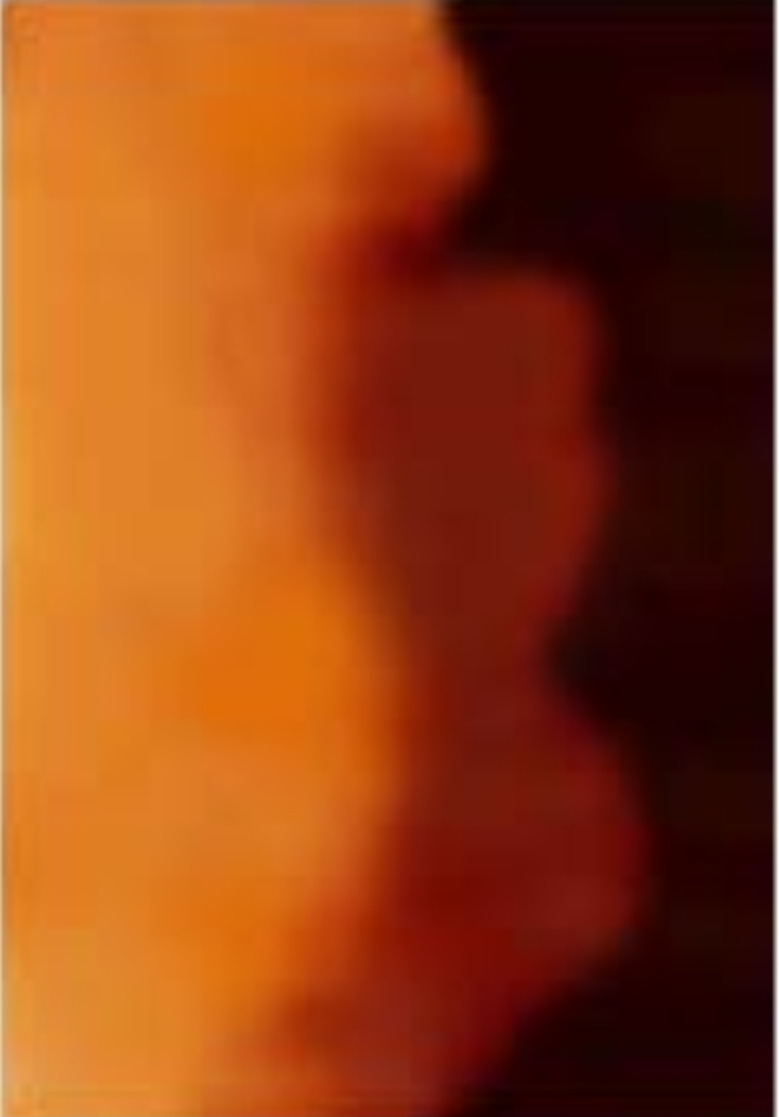
\includegraphics[width = 3.6cm]{Introduction/graphene.png}
\hspace{3cm}
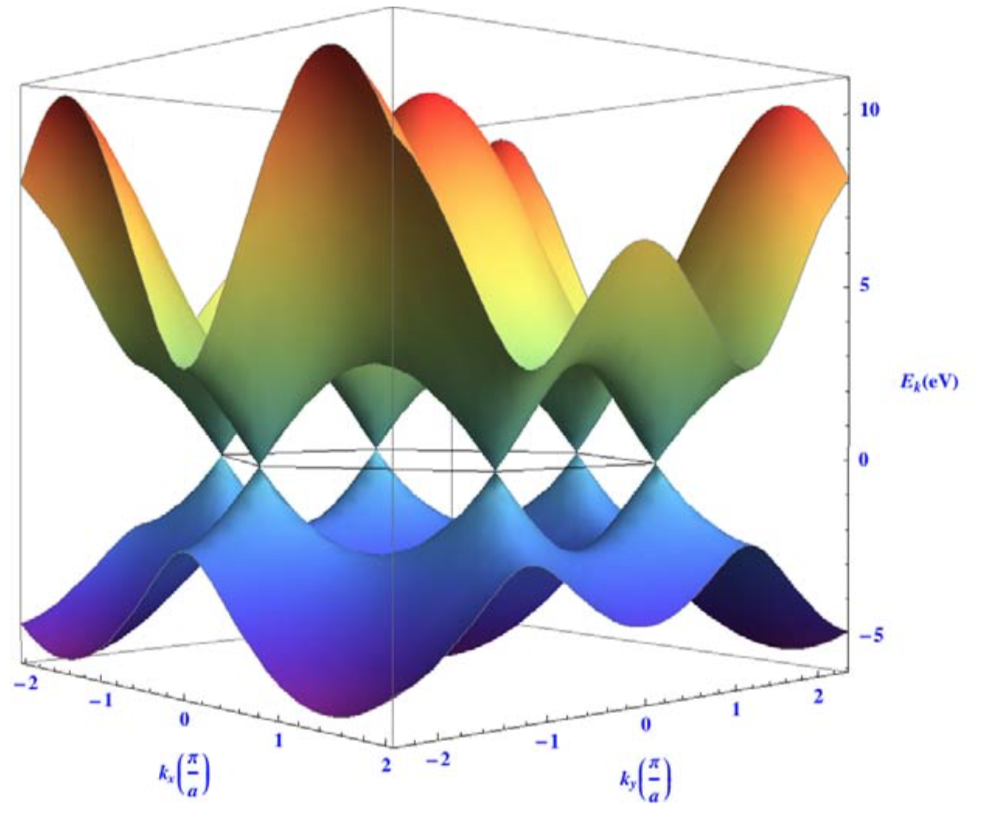
\includegraphics[width = 6.5cm]{Introduction/disp_rel.png}
\caption[Graphene monolayer; graphene's dispersion relation.]{Left: \acf{AFM} picture of a graphene monolayer. The black area is a substrate used for fabrication purposes. The dark orange area is a monolayer of graphene. Right: Dispersion relation of graphene. The black line represents the Fermi energy. Close to it, the dispersion relation is linear, corresponding to massless excitations (taken from \cite{noauthor_nobel_nodate}). }
\label{fig:graphene}
\end{figure}	

On the other hand, \acp{TMD} are a recent member of the \ac{2D} materials family \cite{wang_electronics_2012, roldan_electronic_2014, xu_spin_2014}.
\acp{TMD} have been attracting interest because they seem to overcome some of the drawbacks of graphene in technological applications.
For example, monolayer graphene is gapless, while its bilayer counterpart has only a tunable, but small gap of the order of a tenth of an $eV$.
Contrastingly, \acp{TMD} have an intrinsic gap in excess of $1 \, eV$, being more promising in designing, for example, transistors.
Hole-doped \acp{TMD} are expected to show topological superconductivity \cite{hsu_topological_2017}, while the superconducting phase of graphene has been predicted, but is not easily attained.
Superconductivity in graphene-like \ac{2D} materials is important because it could boost high speed nanoelectronics.
Moreover, the presence of transition metal atoms in \acp{TMD} suggests the possibility of magnetic ordering \cite{braz_valley_2017}, which could be very relevant in nanospintronics applications.
Both topological superconductivity and magnetic ordering arise due to the effect of strong electron correlations.
Thus, to investigate these properties of \acp{TMD} when performing simulations, we need a computational method that is robust enough to capture the effects of electron interactions.

A nanoribbon consists of a \ac{2D} layer that can be regarded as infinitely long on one direction, but not on the other (Figure \ref{fig:fabrication}), so that edge states become relevant, and can be controlled to yield interesting properties.
For simulation purposes, it is natural to assume translational invariance along the ribbon's longitudinal direction, and use \acp{PBC}.
On the other direction, we use \acp{OBC}, effectively considering zigzag edges (Figure \ref{fig:nanoribbons}, left).

\begin{figure}[H]
\centering
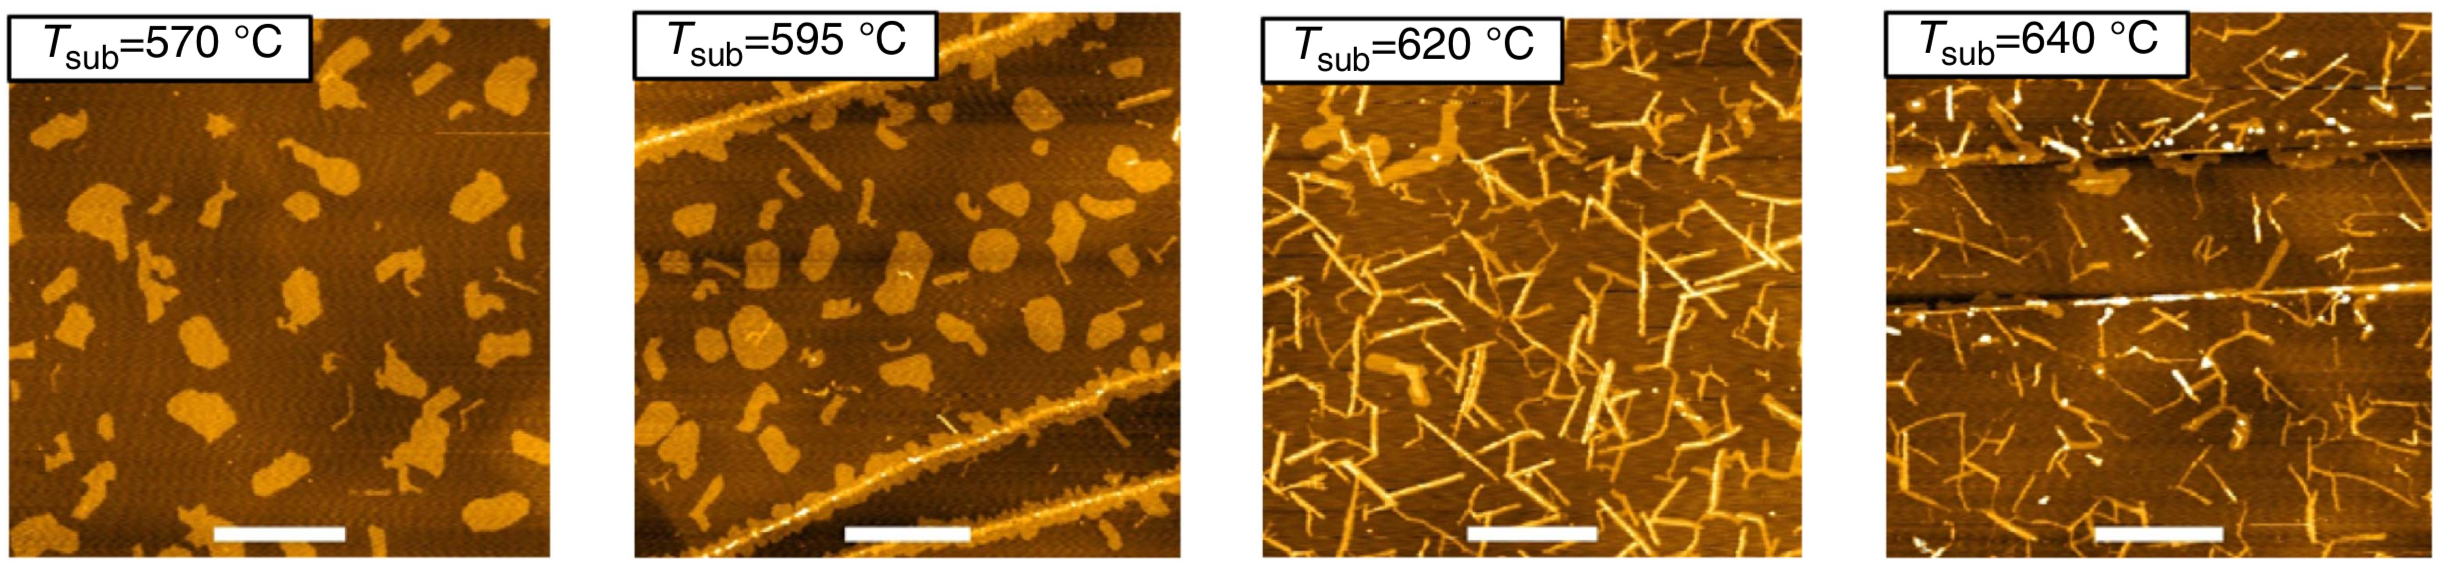
\includegraphics[scale = 0.35]{Introduction/nanoribbons}
\caption[Fabrication of \ac{TMD} nanoribbons]{Fabrication of \ac{TMD} nanoribbons. From left to right, we see \ac{AFM} images showing the appeareance of nanostructures ranging from \ac{2D} nanoislands to nanoribbons, as the temperature of the substrate is increased. The nanoribbons are grown by taking advantage of the temperature dependence of shape transformations occuring during the nonequilibrium growth of this kind of surface-based nanostructures. (taken from \cite{chen_fabrication_2017})}
\label{fig:fabrication}
\end{figure}
   
A high density of low-energy electronic states is localized at the zigzag edges, decaying quickly in the bulk, which suggests the possibility of magnetic ordering.
In fact, a mean field solution of the Hubbard model for a graphene nanoribbon shows that magnetic moments are localized at the edges \cite{yazyev_emergence_2010} (Figure \ref{fig:nanoribbons}, right).
QMC has been used to investigate edge-state magnetism beyond mean field in graphene \cite{feldner_dynamical_2011, golor_quantum_2013, cheng_strain-induced_2015, raczkowski_interplay_2017, yang_strain-tuning_2017}.
However, edge magnetism in TMD nanoribbons remains unexplored \cite{davelou_nanoribbon_2017}.
 
\begin{figure}[H]
\hspace{2cm}
\begin{minipage}[c]{0.1\textwidth}
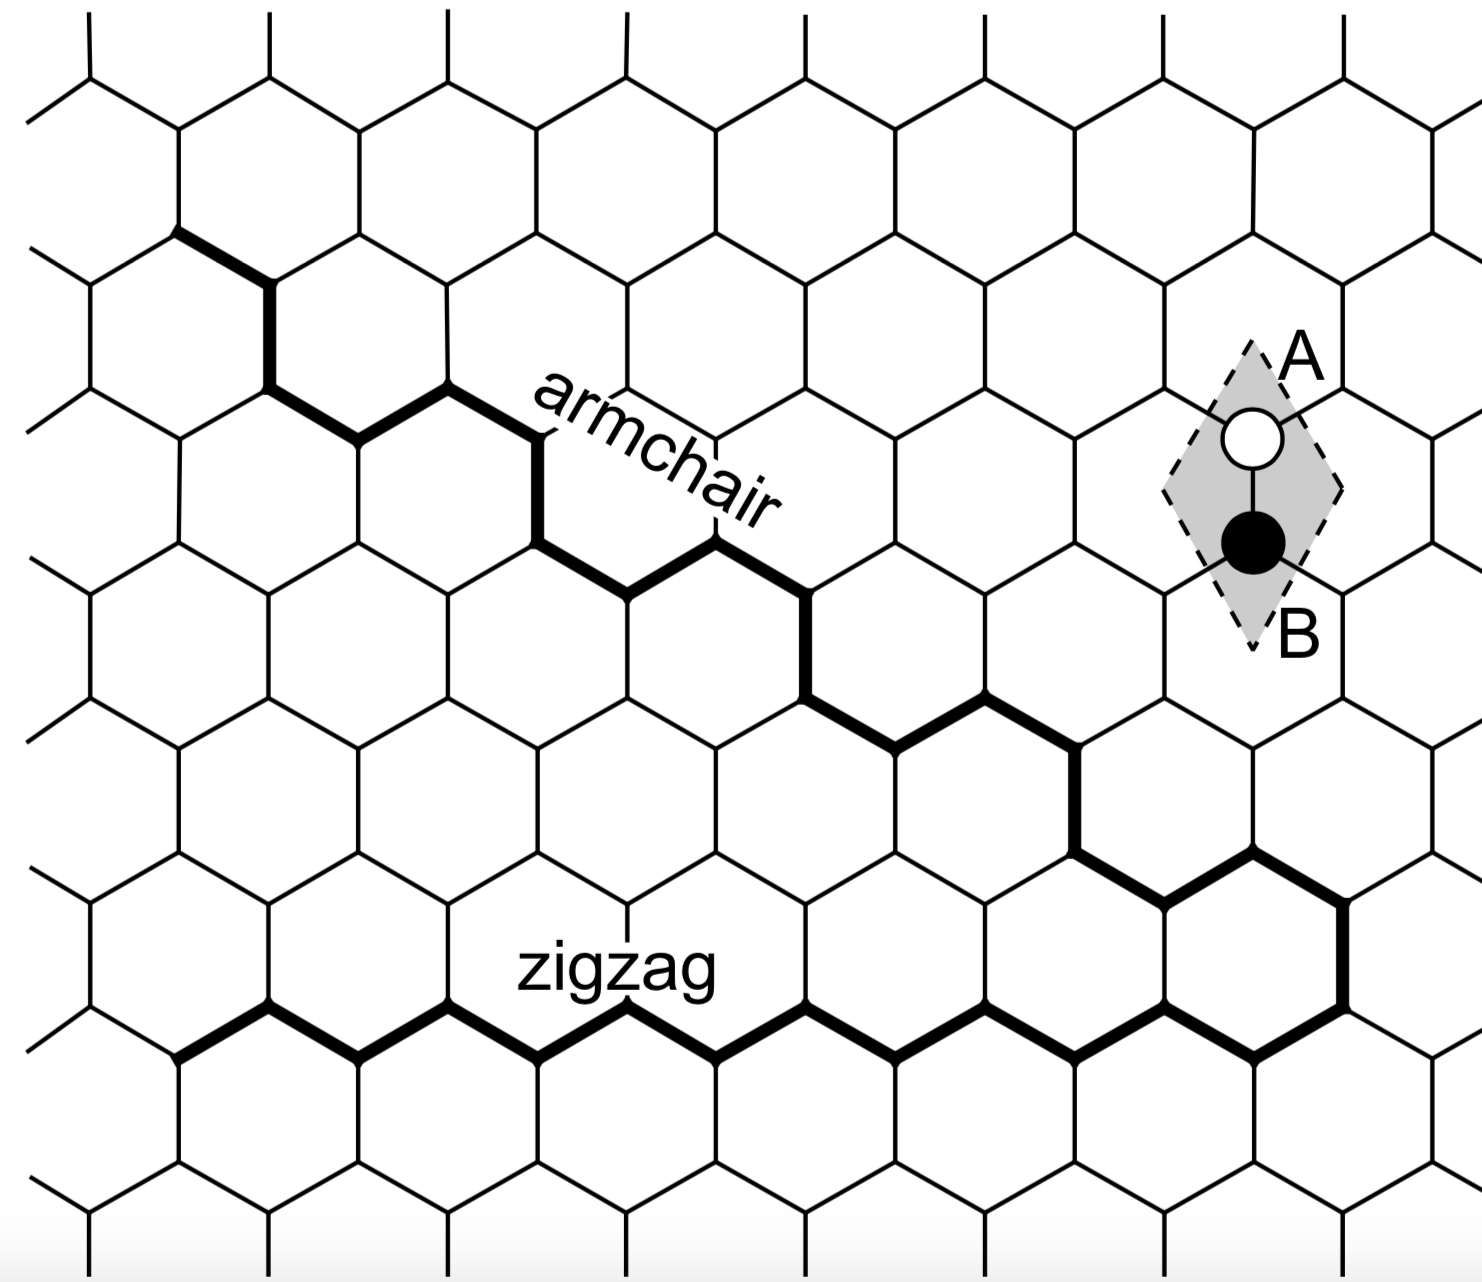
\includegraphics[scale = 0.22]{Introduction/zigzag}
\end{minipage} \hspace{6cm}
\begin{minipage}[c]{0.1\textwidth}
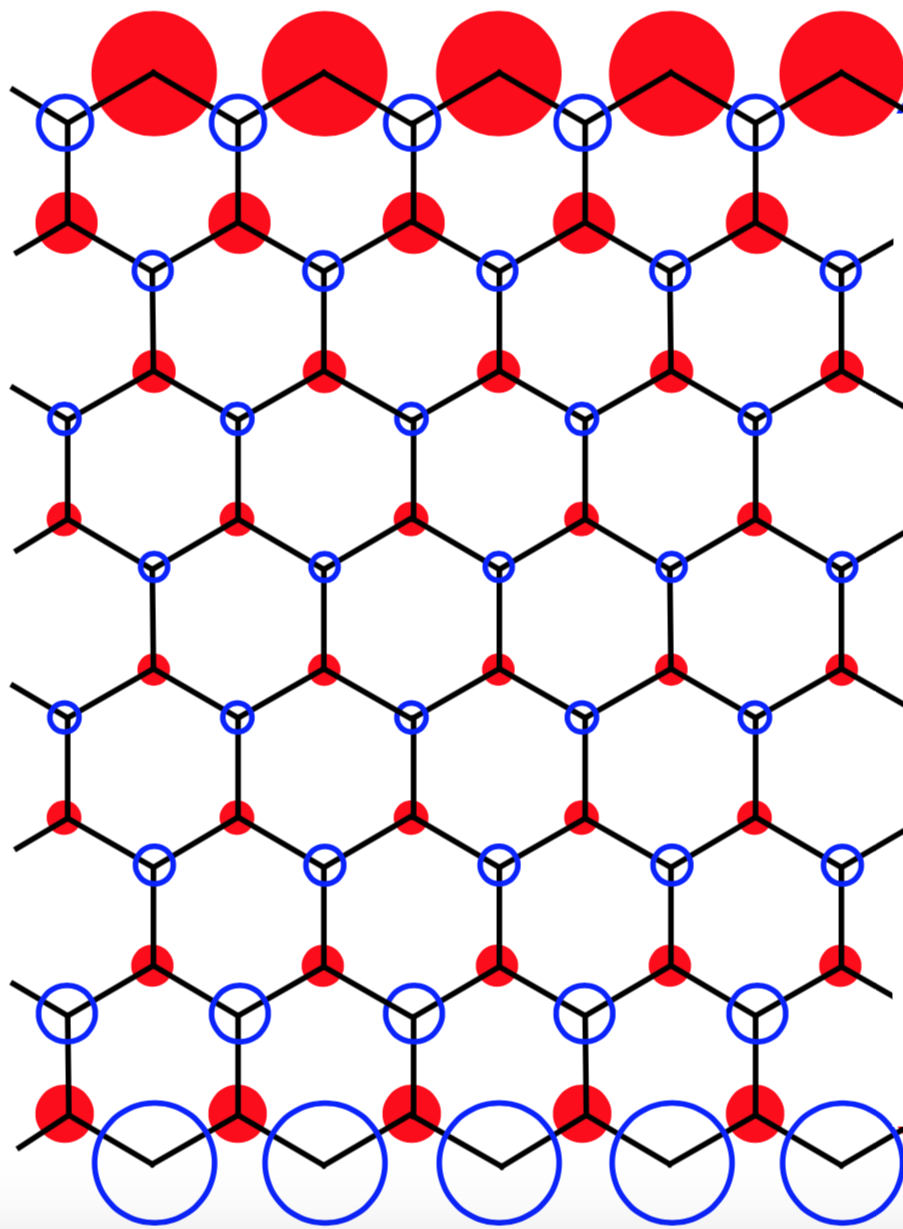
\includegraphics[scale = 0.23]{Introduction/edge_states}
\end{minipage}
 \caption[Zigzag edges of a nanoribbon and magnetism.]{Left: Two possible terminations of a \ac{TMD} nanoribbon condensing in a honeycomb lattice. Right: Local magnetic moments exist on the zig zag edges. The area of the circles corresponds to the magnitude of the magnetic moment, while the color red corresponds to a spin up density, and blue to a spin down density. The accumulation of electronic edge states leads to an \ac{AF} ground state (opposite edges with opposite magnetic moment). (taken from \cite{yazyev_emergence_2010}) \label{fig:nanoribbons}}
\end{figure}

While the zigzag graphene nanoribbon antiferromagnetic ground state is semiconducting, a state with interedge ferromagnetic orientation is a metal.
An example of an application based on the switching between the two states is a magnetorresistive sensor.
This device allows switching between low and high-resistance configurations, corresponding, respectively, to parallel, and antiparallel configurations of ferromagnetic leads at the ends of a nanoribbon.
An important application of this project is precisely the investigation of the possibility of edge-state magnetism, as is observed in graphene nanoribbons, for TMD nanoribbons, which could yield similarly innovative applications.


\subsection{Introduction to \acl{QMC}}

In principle, the properties of a quantum many-fermion system can all be deduced by solving an extremely complicated Schr\"odinger equation that takes into account the coupling of all (identical) particles of the system.
However, for the majority of systems the resulting integrals have no analytic solution, so we solve the problem by numerical integration.
But there is a myriad of methods to evaluate integrals numerically.
How do we pick the best one for this case? 
Multi-dimensional integrals are plagued by the curse of dimensionality.
Although the Newton-Cotes quadrature formulas (including, for example the Newton method, and Simpson's rules), Gaussian quadrature formulas, or Romberg's method all scale polynomially with the number of integration points, they become impractical as the dimension increases.
To use them, one would invoke Fubini's theorem to reduce the multi-dimensional integral to a series of one-dimensional integrals.
However, the number of function evaluations required to compute the whole integral grows exponentially with its dimension.
The Monte Carlo method preserves the polynomial scaling, thus yielding comparable accuracy with far less function evaluations.
It is natural to use it since typically the state space of our quantum system is huge, leading to high dimensional integrals.

The Monte Carlo method is ubiquitous.
Its central idea is to use randomness to produce accurate estimates of deterministic integrals.
The term was coined by Nicolas Metropolis in 1949, first appearing in a seminal paper, in which it was described as a \say{statistical approach to the study of differential equations, or more generally, of integro-differential equations that occur in various branches of sciences}\cite{metropolis_monte_1949}.
Although it was used as early as 1777 in an experiment known as Buffon's needle - where one obtains an estimate of the constant $\pi$ by repeatedly throwing a needle randomly onto a sheet of paper with evenly spaced lines - it was crucially developed in the Los Alamos National Laboratory during World War II where the development of the first atomic bomb was completed, the primary objective of the Manhattan Project.
The method is particularly useful when one wants to sample from a probability distribution in an exponentially large state space.
In fact, it can in principle be used to solve any problem allowing a probabilistic formulation.

A variety of \acf{QMC} methods exists, using a sampling scheme based on the Metropolis algorithm, and variations thereof.
Variational and Diffusion \ac{QMC} are the simplest \ac{QMC} methods that allow one to capture some properties of correlated systems.
Although they already contain the main concepts used in this type of simulations, it is not always possible to use them. 
We will discuss their flaws and show how further refinement leads to the determinant, or auxiliary field method we ultimately used.

Using the Monte Carlo approach to study a many-fermion system implies overcoming a significant obstacle common to all \ac{QMC} methods - the so called \emph{fermion-sign problem}.
Pauli's exclusion principle implies that the many-fermion wave function is anti-symmetric, which leads to a sign oscillation that greatly impedes the accurate evaluation of averages of quantum observables.
The anti-symmetry constraint implies that a  straightforward weight interpretation of the wave function is not possible.
In the case of the finite temperature algorithm, the cancellations that occur when computing the average of any physical observable lead to poor statistical properties of the corresponding estimators.
This means that a massive amount of samples requiring enormous computer time are needed to obtain meaningful results.
In the case of the zero temperature algorithms, the situation is even worse.
It might not even be possible to design a stochastic process carrying the system to its ground state, as normally is done in \say{projective} methods\footnote{Methods that iteratively project a trial wave function onto the ground state.}: the wave function that is used as an initial proposal turns out to converge to a bosonic one, and the fermionic character of the system is lost.

As was proven by Troyer, the \emph{fermion-sign problem} has NP\footnote{NP or nondeterministic polynomial time, meaning that one can devise an algorithm that verifies the "yes" answer to a decision problem in polynomial time in the system size.
Note that the class $P$ - of polynomial time algorithms - is a subclass of NP.} computational complexity \cite{troyer_computational_2005}.
One of the greatest open questions in computer science is whether $P = NP$.
Solving the \emph{fermion-sign problem} would imply finding a solution to $P = NP$, which would constitute a major breakthrough.



\subsection{Variational Monte Carlo}

Variational techniques rely on an educated guess for the wave function of the system.
One introduces a set of variational parameters $\bm \alpha$ that are then tuned according to a variational principle.
Then, we may use the optimized trial wave function to compute physical quantities of interest using Monte Carlo.
The method is used to obtain zero temperature properties of a given model.
Note that it requires prior knowledge about the system to propose an approximate wave function in the first place.

A particularly relevant observable is the variational energy $E_V$ associated to a trial ground state.
Let $\bm r$ be the $3N$ spatial coordinates of the $N$ electrons.
Given the Hamiltonian of the system $\mathcal{H}$, and a trial wave function $\psi (\bm r)$ - a guess of the wave function representing the ground state - one can compute the corresponding variational energy.

\begin{equation}\label{eq:variational_energy}
E_V = \frac{\left\langle \psi | \mathcal{H} | \psi \right \rangle}{\left\langle \psi | \psi \right \rangle} = \frac{ \int d\bm r |\psi (\bm r)|^2 E_L (\bm r)}{\int d\bm r | \psi (\bm r)|^2 } = \int d\bm r\rho (\bm r) E_L (\bm r) ,
\end{equation}
where the local energy $E_L (\bm r)$ is defined as

\begin{equation}\label{eq:local_energy}
E_L = \frac{\mathcal{H} \psi (\bm r) }{\psi (\bm r)}
\end{equation}
and the probability distribution $\rho (\bm r)$ is defined as

\begin{equation}\label{eq:rho}
\rho (\bm r) = \frac{ | \psi (\bm r) |^2}{ \int d\bm r' | \psi (\bm r') |^2}
\end{equation}

Note that we managed to recast the variational energy as an average of the \emph{local} energy, $\left\langle E_L \right\rangle $, over the the distribution $\rho$.
This may be computed using the Monte Carlo method by sampling $M$ points $\bm r_k$ from distribution $\rho (\bm r)$:

\begin{equation}\label{eq:average}
E_V \approx \overline{E}_L = \frac{1}{M} \sum_{k= 1}^{M} E_L (\bm r_k) ,
\end{equation}
where $\overline {X}$ denotes a sample mean of the random variable $X$.

Let the ground state energy be $E_0$.
Then, states are optimized according to the variational principle:

\begin{equation}
E_V(\bm \alpha) = \frac{\left\langle \psi_{\bm \alpha} | \mathcal{H} | \psi_{\bm \alpha} \right\rangle}{\left\langle\psi_{\bm \alpha} | \psi_{\bm \alpha} \right\rangle} \ge E_0,
\end{equation}
where $\psi_{\bm \alpha}$ is the trial ground state wave function for the set of variational parameters ${\bm \alpha}$.

By varying $\bm \alpha$ we aim to obtain a variational energy that is as close as possible to the true ground state energy.
Since $E_V(\bm \alpha)$ is bounded from below, this is equivalent to minimizing it in the hope that $E_V(\bm \alpha_{min}) \gtrsim E_0$, i.e. the bound is tight.

The finite sampling size $M$, of course, introduces a statistical error common to all Monte Carlo methods. 
However, the use of an approximate wave function introduces a systematic error that is hard to control since trial wave functions are generally introduced based on approximate, or heuristic arguments.

\subsection{Diffusion Monte Carlo and projective methods}\label{subsec:dmc}

Variational Monte Carlo is severely limited by the use of a trial wave function $\psi_{\bm \alpha} (\bm r)$ because we may even not have enough information to even construct a reliable variational wave function.

Diffusion \ac{QMC} allows the simulation of a many-body system while having only a limited knowledge of the system's physical properties.
While it is exact for many-boson systems, it is only approximate for many-fermion systems.
The idea is to map the Schr\"odinger equation into  an imaginary-time diffusion equation.
Excited states are then filtered out by a diffusion process as we advance in imaginary-time.
In imaginary-time $\tau = i t$, the solution to the Schr\"odinger equation in terms of a formal series expansion in the eigenfunctions of the hamiltonian becomes a series of transients $e^{-E_n \tau}, \, n \in \mathbb{N}$.
The longest lasting of these is the ground state  \cite{kosztin_introduction_1996}.

The idea of the diffusion method is to generate samples using the exact ground state wave function $\psi_0 (\bm r)$ \cite{toulouse_chapter_2016}.
The associated exact energy $E_0$ is the matrix element of the hamiltonian calculated using a trial wave function and the ground state wave function.

\begin{equation}
E_0 = \frac{ \left\langle \psi_0 |E_0 \mathbbm{1} | \psi \right\rangle}{\left\langle \psi_0 | \psi \right\rangle} = \frac{\left\langle \psi_0 | \mathcal{H} | \psi \right\rangle}{ \left\langle\psi_0 | \psi \right\rangle} = \frac{\int d\bm r \psi_0^\star (\bm r) \psi (\bm r) E_L (\bm r)}{\int d\bm r\psi_0^\star (\bm r) \psi (\bm r)}
\end{equation}

Note that using this trick we avoid the computation of $\mathcal{H} \psi_0 = E_0 \psi_0$, that is, the ground state energy.
Instead, we approximate the integral by considering $M$ configuration samples $\bm r_{k = 1,..., N}$ in a similar spirit to that of Variational \ac{QMC}.
Notice that the integral consists of a local energy of the trial wave function $E_L (\bm r) = \frac{\mathcal{H} \psi (\bm r)}{\psi (\bm r)}$ averaged over a mixed distribution from which we draw a sample of points $\bm r_{k=1,...M}$:

\begin{equation}
f(\bm r) = \frac{\psi_0^\star (\bm r) \psi (\bm r) }{ \int d\bm r  \psi_0 (\bm r) \psi (\bm r)}
\end{equation}

Although the method is, of course, aimed at probing many-body systems, let us consider a single particle in \acs{1D} for simplicity for illustrating the method.
Performing a Wick rotation - effectively going to imaginary time - and shifting the energy, the Schr\"odinger equation becomes

\begin{equation}
\frac{\partial \psi ( x, \tau )}{\partial\tau}  = -\frac{1}{2m}\frac{\partial^2 \psi ( x, \tau )}{\partial x^2} - \bigg[ V(x) - E_T \bigg] \psi( x, \tau ) 
\end{equation}

The exact ground state wave function $\psi_0 ( x )$ is obtained as the longest lasting transient state in imaginary time: we are interested in the asymptotic behavior of the series expansion constituting the formal solution of the Schr\"odinger equation

\begin{equation}
\psi (x, \tau) = \sum_{n=0}^{\infty} c_n \psi_n (x) e^{-(E_n - E_T)\tau}
\end{equation}

Imaginary time evolution is governed by

\begin{equation}\label{eq:im_ev}
\begin{split}
&\left| \psi (t) \right\rangle = \lim_{\tau \rightarrow \infty} \sum_i e^{-(E_i - E_T) \tau} \left|\psi_i \right\rangle \left\langle \psi_i | \psi \right\rangle = \\
&= \lim_{\tau \rightarrow \infty} e^{-(E_0 - E_T)\tau} \left| \psi_0 \right\rangle \left\langle \psi_0 | \psi \right\rangle 
\end{split}
\end{equation}


If $E_T > E_0$ the wave function diverges exponentially fast: $\lim_{\tau \rightarrow \infty} \psi ( x, \tau) = \infty$.
Similarly, for $E_T < E_0$ it vanishes exponentially fast: $\lim_{\tau \rightarrow \infty} \psi ( x, \tau) = 0$.
However, if $E_T = E_0$ the wave function converges to the ground state one up to a constant factor.

\begin{equation}\label{eq:dmc}
\lim_{\tau \rightarrow \infty} \psi ( x, \tau) = c_0 \psi_0 (x) \,\,\, \text{, or} \quad \lim_{\tau \rightarrow \infty} \left|\psi (\tau) \right\rangle \propto \left| \psi_0 \right\rangle
\end{equation}

Diffusion \ac{QMC} makes use of Eq. (\ref{eq:dmc}), approximating $\psi_0(x)$ by $\psi (x, \tau)$ for sufficiently long time.
The only requirement is that $\psi (x, \tau)$ and $\psi_0(x)$ overlap significantly so that $c_0$ is large enough to be numerically measurable, and we can always center a positive trial wave function in a region where $\psi_0(x)$ is large enough and positive.
If the latter condition does not hold, the wave function converges to a bosonic, instead of a fermionic one.
Of course, these conditions can always be met for a single particle, but note that they might fail for a many-fermion system, for which the wave function crosses a number of nodes due to its anti-symmetric nature.

\subsection{Drawbacks of variational and projective methods. Auxiliary Field \acs{QMC}. The Fermion Sign Problem.}
\label{subsec:introAFQMC}

As we have seen, the major drawback of the variational method was that it demanded \emph{a priori} knowledge of a reasonable variational wave function describing, at least partly, some of the physics of the problem.
Diffusion \acs{QMC} demands less: we need only propose a trial wave function that overlaps with the ground state.
However, none of these methods allow us to probe systems at finite temperature.
Moreover, they both require some prior knowledge about the system, which may not always be available.

An alternative method is based on introducing an additional lattice bosonic field that mediates the electron-electron interaction.
The interacting problem then becomes a problem of independent fermions coupled to an external field, and the fermionic part of the partition function can be traced out explicitly, leaving the contribution of a \emph{discrete}\footnote{Although, there is a finite number of field configurations, the number grows exponentially with the number of sites on the lattice.} bosonic field.
This contribution can be evaluated numerically by employing importance sampling over the field configurations.
Auxiliary field \acs{QMC} relies on a mapping to a classical system:

\begin{equation}
Z = \Tr [ e^{-\beta \mathcal{H} } ] = \sum_c p_c ,
\end{equation}
but some of the \say{probabilities} can actually be negative $p_c < 0$.
This occurs due to the antisymmetry of the many-electron wave function under exchange of two electrons.

The negative weight problem may easily be circumvented when computing averages of observables:

\begin{equation}\label{eq:signSampling}
\left\langle A \right\rangle = \frac{\sum_c A ( c ) p ( c )}{\sum_c p ( c ) } = \frac{\sum_c A ( c )|  p ( c ) | \text{sign}[p(c)] / \sum_c | p ( c ) | }{\sum_c  |  p ( c ) | \text{sign}[p(c)] /  \sum_c | p ( c ) |} \equiv \frac{\left\langle A s \right\rangle_{|p|}}{\left\langle s \right\rangle_{|p|}} ,
\end{equation}
where $s(c) = \text{sign} [ p ( c ) ]$, and $| p ( c ) | $ corresponds to an auxiliary bosonic system (also coupled to the bosonic field) corresponding to the original fermionic system, and for which there is no sign problem.

The relative error $\Delta s / \left\langle s \right\rangle$ increases exponentially with the number of particles, with inverse temperature, and possibly with other parameters of the specific model to be studied \cite{troyer_computational_2005, hou_numerical_2009}.
To see this, we start by noting that the average sign is the ratio between the partition functions of the fermionic ($Z = \sum_c p(c)$) and bosonic systems ($Z = \sum_c | p ( c ) |$).
In terms of the difference in free energy densities, $\left\langle s \right\rangle = Z / Z' = e^{-\beta N_p \Delta f}$, implying that for $M$ samples, the error of the denominator of Eq. (\ref{eq:signSampling}) becomes

\begin{equation}
\frac{\Delta s}{\left\langle s \right\rangle} = \frac{\sqrt{(\left\langle s^2 \right\rangle - \left\langle s \right\rangle^2 )/ M }}{\left\langle s \right\rangle} = \frac{ \sqrt{ 1 - \left\langle s \right\rangle^2}  }{\sqrt{M} \left\langle s \right\rangle} \propto \frac{e^{\beta N_p \Delta f}}{\sqrt{M}} ,
\end{equation}
and similarly for the numerator of Eq. (\ref{eq:signSampling}).

Auxiliary field \acs{QMC} can also be formulated to probe ground state properties, and a sign problem arises similarly.
Apart from this problem, which plagues all \acs{QMC} methods, this method is one of the most robust, unbiased, and reliable methods, hence we choose it to carry out our simulations.
Note that, in particular, it is certainly more powerful than the variational and diffusion methods outlined before since it requires much less \emph{a priori} information about the system.
Perhaps more importantly, given some recent findings, it can be used in conjunction with neural networks to discover quantum phase transitions in correlated systems  \cite{broecker_machine_2017}.
\section{Introduction to \acl{QMC}}
\label{sec:introQMC}

Solving the many-body problem remains one of the greatest challenges in physics.
Following the wealth of attempts at such pursuit, certain phenomena arising due to the strong interactions in quantum systems are explained in different theoretical frameworks, namely superconductivity, the Mott metal-insulator transition, and fractional quantum Hall effect.
All of these breakthroughs represented revolutions in their respective fields with significant scientific and technological impact.
However, only in very limited cases does an actual analytical solution exist for the  Schr\"odinger equation for a system of interacting particles.
One must resort to sophisticated approximation methods to obtain  information about the role played by the competing interactions under various conditions in the aforementioned cases.
It is then natural that numerical methods have become prominent as a tool for extracting useful information about this type of systems.
\ac{QMC} is amongst the most accurate and extensively studied ones.
The idea of all \ac{QMC} methods is to reduce the interacting problem to solving a set of integrals, which can be evaluated numerically through a standard stochastic procedure.
These integrals are arrived at upon formulating the quantum many-body description of the system using the Schr\"odinger equation.
Hence the name \acl{QMC}, which is used to distinguish it from Classical Monte Carlo.
In the classical version, one measures thermal averages, while in the quantum version, one measures expectations of operators over the Hilbert space of the system, corresponding to physical observables that fluctuate with a dynamics given by the Schr\"odinger equation (and, of course, can also have thermal fluctuations).
In fact, the dynamics of a quantum system are encoded in the Hamiltonian operator.
In the case of graphene-like \ac{2D} materials, one usually uses a tight-binding model.
It is found that the dynamics given by the tight-binding Hamiltonian is sufficient to describe most properties of graphene.
However, in other materials, such as \acp{TMD}, electron-electron interactions are stronger, and Hubbard-type models could give us a more accurate picture of the phenomena that occur within them.

For quantum many-fermion systems, observables are given in terms of integrals which have no analytic solution, so we solve the problem numerically.
But there is a myriad of methods to evaluate integrals numerically.
How do we pick the best one for this case? 
Multi-dimensional integrals are plagued by the curse of dimensionality.
Although the Newton-Cotes quadrature formulas (including, for example the Newton method, and Simpson's rules), Gaussian quadrature formulas, or Romberg's method all scale polynomially with the number of integration points, they become impractical as the dimension increases.
To use them, one would invoke Fubini's theorem to reduce the multi-dimensional integral to a series of one-dimensional integrals.
However, the number of function evaluations required to compute the whole integral grows exponentially with its dimension.
The Monte Carlo method preserves the polynomial scaling, thus yielding comparable accuracy with far less function evaluations.
It is natural to use it since typically the state space of our quantum system is huge, leading to high dimensional integrals.

The Monte Carlo method is ubiquitous.
Its central idea is to use randomness to produce accurate estimates of deterministic integrals.
The term was coined by Metropolis in 1949, although it was used as early as 1777 in an experiment known as Buffon's needle - where one obtains an estimate of the constant $\pi$ by repeatedly throwing a needle randomly onto a sheet of paper with evenly spaced lines. %t was crucially developed in the Los Alamos National Laboratory during World War II where the development of the first atomic bomb was completed, the primary objective of the Manhattan Project.
The method is particularly useful when one wants to sample from a probability distribution in an exponentially large state space (like the huge Hilbert space of an interacting electron system), but it can, in principle, be used to solve any problem allowing a probabilistic formulation.
To solve the interacting fermion problem, a variety of \ac{QMC} methods exists, using a sampling scheme based on the Metropolis algorithm, and variations thereof.
Variational and Diffusion \ac{QMC} are the simplest \ac{QMC} methods that allow one to capture some properties of correlated systems, but it is not always ideal or even possible to use them. 
%We will discuss their flaws and show how further refinement leads to the auxiliary field method we ultimately used.

Using the Monte Carlo approach to study a many-fermion system implies overcoming a significant obstacle common to all \ac{QMC} methods - the so called \emph{fermion sign problem}.
Pauli's exclusion principle implies that the many-fermion wave function is anti-symmetric, which leads to a sign oscillation that greatly impedes the accurate evaluation of averages of quantum observables.
The anti-symmetry constraint implies that a  straightforward weight interpretation of the wave function is not possible.
In the case of the finite temperature algorithm, the cancellations that occur when computing the average of any physical observable lead to poor statistical properties of the corresponding estimators.
This means that a massive amount of samples requiring enormous computer time are needed to obtain meaningful results.
In the case of the zero temperature algorithms, the situation is even worse.
It might not even be possible to design a stochastic process carrying the system to its ground state, as normally is done in \say{projective} methods\footnote{Methods that iteratively project a trial wave function onto the ground state.}: the wave function that is used as an initial proposal turns out to converge to a bosonic one, and the fermionic character of the system is lost.
As was proven by Troyer, the \emph{fermion sign problem} has NP\footnote{NP or nondeterministic polynomial time, meaning that one can devise an algorithm that verifies the "yes" answer to a decision problem in polynomial time in the system size.
Note that the class $P$ - of polynomial time algorithms - is a subclass of NP.} computational complexity \cite{troyer_computational_2005}.
One of the greatest open questions in computer science is whether $P = NP$.
Solving the \emph{fermion sign problem} would imply finding a solution to $P = NP$, which would constitute a major breakthrough.

\subsection{Variational Monte Carlo}

Variational techniques rely on an educated guess for the wave function of the system.
One introduces a set of variational parameters $\bm \alpha$ that are then tuned according to a variational principle.
Then, we may use the optimized trial wave function to compute physical quantities of interest using Monte Carlo.
The method is used to obtain zero temperature properties of a given model.
Note that it requires prior knowledge about the system to propose an approximate wave function in the first place.

A particularly relevant observable is the variational energy $E_V$ associated to a trial ground state.
Let $\bm r$ be the $3N$ spatial coordinates of the $N$ electrons.
For simplicity, let us ignore all other degrees of freedom, such as spin.
Given the Hamiltonian of the system $\mathcal{H}$, and a trial wave function $\psi_T (\bm r)$ - a guess of the wave function representing the ground state - one can compute the corresponding variational energy by averaging over a \say{local} energy:

\begin{equation}\label{eq:variational_energy}
E_V = \frac{\left\langle \psi_T | \mathcal{H} | \psi_T \right \rangle}{\left\langle \psi_T | \psi_T \right \rangle} = \frac{ \int d\bm r |\psi_T (\bm r)|^2 E_L (\bm r)}{\int d\bm r | \psi_T (\bm r)|^2 } = \int d\bm r\rho (\bm r) E_L (\bm r) , \text{where}
\end{equation}

\begin{equation}\label{eq:local_energy}
E_L = \frac{\mathcal{H} \psi_T (\bm r) }{\psi_T (\bm r)}   \quad \text{and} \quad \rho (\bm r) = \frac{ | \psi_T (\bm r) |^2}{ \int d\bm r' | \psi_T (\bm r') |^2}
\end{equation}

Note that we managed to recast the variational energy as an average of the \emph{local} energy, $\left\langle E_L \right\rangle $, over the the distribution $\rho$.
This may be computed using the Monte Carlo method by sampling $M$ points $\bm r_k$ from the distribution $\rho (\bm r)$.
Denoting the sample mean of the random variable $X$ as $\overline {X}$:

\begin{equation}\label{eq:average}
E_V \approx \overline{E}_L = \frac{1}{M} \sum_{k= 1}^{M} E_L (\bm r_k) ,
\end{equation}

Let the ground state energy be $E_0$.
Then, states are optimized according to the variational principle:

\begin{equation}
E_V(\bm \alpha) = \frac{\left\langle \psi_{\bm \alpha} | \mathcal{H} | \psi_{\bm \alpha} \right\rangle}{\left\langle\psi_{\bm \alpha} | \psi_{\bm \alpha} \right\rangle} \ge E_0,
\end{equation}
where $\psi_{\bm \alpha}$ is the trial ground state wave function for the set of variational parameters ${\bm \alpha}$.
By varying $\bm \alpha$ we aim to obtain a variational energy that is as close as possible to the true ground state energy, and use the corresponding trial wave function to compute averages of other observables.
Since $E_V(\bm \alpha)$ is bounded from below, this is equivalent to minimizing it in the hope that $E_V(\bm \alpha_{min}) \gtrsim E_0$, i.e. the bound is tight.
The finite sampling size $M$, of course, introduces a statistical error common to all Monte Carlo methods. 
However, the use of an approximate wave function introduces a systematic error that is hard to control since trial wave functions are generally introduced based on approximate, or heuristic arguments.

\subsection{Diffusion Monte Carlo and projective methods}\label{subsec:dmc}

Variational Monte Carlo is severely limited by the use of a trial wave function $\psi_T (\bm r)$ because we may not even have enough information to even construct a reliable variational wave function in the first place.
Diffusion \ac{QMC} allows the simulation of a many-body system while having only a limited knowledge of the system's physical properties.
As a projective method, it is exact for many-boson systems, while being only approximate for many-fermion systems.
The idea is to map the Schr\"odinger equation onto an imaginary-time diffusion equation.
Excited states are then filtered out by a diffusion process as we advance in imaginary-time.
In imaginary-time $\tau = i t$, the solution to the Schr\"odinger equation in terms of a formal series expansion in the eigenfunctions of the Hamiltonian becomes a series of \say{transient} wavefunctions weighted by $e^{-E_n \tau}, \, n \in \mathbb{N}$.
Within precision and accuracy constraints, the longest lasting of these is the ground state \cite{kosztin_introduction_1996}.
Thus, the idea of the diffusion method is to generate samples using the exact ground state wave function $\psi_0 (\bm r)$ \cite{toulouse_chapter_2016}.
The associated exact energy $E_0$ is the matrix element of the hamiltonian calculated using a trial wave function and the ground state.

\begin{equation}
E_0 = \frac{ \big( \left\langle \psi_0 |E_0 \big) \big( \mathbbm{1} | \psi_T \right\rangle \big)}{\left\langle \psi_0 | \psi_T \right\rangle} = \frac{\left\langle \psi_0 | \mathcal{H} | \psi_T \right\rangle}{ \left\langle\psi_0 | \psi_T \right\rangle} = \frac{\int d\bm r \psi_0^\star (\bm r) \psi_T (\bm r) E_L (\bm r)}{\int d\bm r\psi_0^\star (\bm r) \psi_T (\bm r)}
\end{equation}

Note that using this trick we avoid the computation of $\mathcal{H} \psi_0 = E_0 \psi_0$, that is, the ground state energy.
Instead, we approximate the integral by considering $M$ configuration samples $\bm r_{k = 1,..., M}$ in a similar spirit to that of Variational \ac{QMC}.
Notice that the integral consists of a local energy of the trial wave function $E_L (\bm r) = \frac{\mathcal{H} \psi (\bm r)}{\psi (\bm r)}$ averaged over a mixed distribution from which we draw a sample:

\begin{equation}
f(\bm r) = \frac{\psi_0^\star (\bm r) \psi_T (\bm r) }{ \int d\bm r  \psi_0 (\bm r) \psi_T (\bm r)}
\end{equation}

Although the method is, of course, aimed at probing many-body systems, let us consider a single particle in \acs{1D}, for simplicity, to illustrate the method.
Performing a Wick rotation - effectively going to imaginary time - and shifting the energy, the Schr\"odinger equation becomes (with $\hbar = 1$)

\begin{equation}
\frac{\partial \psi_T ( x, \tau )}{\partial\tau}  = -\frac{1}{2m}\frac{\partial^2 \psi_T ( x, \tau )}{\partial x^2} - \bigg[ V(x) - E_T \bigg] \psi_T( x, \tau ) 
\end{equation}

The exact ground state wave function $\psi_0 ( x )$ is obtained as the longest lasting transient state in imaginary time: we are interested in the asymptotic behavior of the series expansion constituting the formal solution of the Schr\"odinger equation

\begin{equation}
\psi_T (x, \tau) = \sum_{n=0}^{\infty} c_n \psi_n (x) e^{-(E_n - E_T)\tau}
\end{equation}

Imaginary time evolution is governed by

\begin{equation}\label{eq:im_ev}
\left| \psi_T (t) \right\rangle = \lim_{\tau \rightarrow \infty} \sum_n e^{-(E_n - E_T) \tau} \left|\psi_n \right\rangle \left\langle \psi_n | \psi_T \right\rangle = \lim_{\tau \rightarrow \infty} e^{-(E_0 - E_T)\tau} \left| \psi_0 \right\rangle \left\langle \psi_0 | \psi_T \right\rangle 
\end{equation}

If $E_T > E_0$ the wave function diverges exponentially fast: $\lim_{\tau \rightarrow \infty} \psi_T ( x, \tau) = \infty$.
Similarly, for $E_T < E_0$ it vanishes exponentially fast: $\lim_{\tau \rightarrow \infty} \psi_T ( x, \tau) = 0$.
However, if $E_T = E_0$ the wave function converges to the ground state one up to a constant factor, $c_0 = \left\langle \psi_0 | \psi_T \right\rangle$.

\begin{equation}\label{eq:dmc}
\lim_{\tau \rightarrow \infty} \psi_T ( x, \tau) = c_0 \psi_0 (x) \quad \text{or} \quad \lim_{\tau \rightarrow \infty} \left|\psi_T (\tau) \right\rangle \propto \left| \psi_0 \right\rangle
\end{equation}

Diffusion \ac{QMC} makes use of Eq. (\ref{eq:dmc}), approximating $\psi_0(x)$ by $\psi_T (x, \tau)$ for sufficiently long time.
The only requirement is that $\psi_T (x, \tau)$ and $\psi_0(x)$ overlap significantly so that $c_0$ is large enough to be numerically measurable, and we can always center a positive trial wave function in a region where $\psi_0(x)$ is large enough and positive.
If the latter condition does not hold, the wave function converges to a bosonic, instead of a fermionic one.
Of course, these conditions can always be met for a single particle, but note that they might fail for a many-fermion system, for which the wave function crosses a number of nodes due to its anti-symmetric nature.

\subsection{Auxiliary Field \acs{QMC} and the Fermion Sign Problem}
\label{subsec:introAFQMC}

As we have seen, the major drawback of the variational method was that it demanded \emph{a priori} knowledge of a reasonable variational wave function describing, at least partly, some of the physics of the problem.
Diffusion \acs{QMC} demands less: we need only propose a trial wave function that overlaps with the ground state.
However, none of these methods allow us to probe systems at finite temperature.
Moreover, they both require some prior knowledge about the system, which may not always be available.

An alternative method is based on introducing an additional lattice bosonic field that mediates the electron-electron interaction.
The interacting problem then becomes a problem of independent fermions coupled to an external field, and the fermionic part of the partition function can be traced out explicitly, leaving the contribution of a \emph{discrete}\footnote{The introduced field is discrete (and \emph{binary}) because each fermionic state can only have occupations $n = 0, 1$. Although, there is a finite number of field configurations, the number grows exponentially with the number of sites on the lattice.} bosonic field, $\bm h$.
This contribution can be evaluated numerically by employing importance sampling over the field configurations.
Auxiliary field \acs{QMC} relies on a mapping to a so called \say{classical} system (in quotes because there may be no actual classical analogue):

\begin{equation}\label{eq:Zsign}
Z = \Tr [ e^{-\beta \mathcal{H} } ] = \sum_{\{ \bm h\} } \sum_{\text{fermionic}} e^{-S} = \sum_c p_c ,
\end{equation}
but some of the \say{probabilities} can actually be negative $p_c < 0$.
This occurs due to the antisymmetry of the many-electron wavefunction under electron exchange, and is at the root of the sign problem.
Here, $S$ is a fermion-boson action that we shall write out explicitly later.
For a fixed configuration of the bosonic field, we sum over the fermionic part exactly to obtain the weight of each configuration $p_c$.
The sum over $\bm h$ is carried out stochastically.

The negative weight problem may easily be circumvented when computing averages of observables:

\begin{equation}\label{eq:signSampling}
\left\langle A \right\rangle = \frac{\sum_c A ( c ) p ( c )}{\sum_c p ( c ) } = \frac{\sum_c A ( c )|  p ( c ) | \text{sign}[p(c)] / \sum_c | p ( c ) | }{\sum_c  |  p ( c ) | \text{sign}[p(c)] /  \sum_c | p ( c ) |} \equiv \frac{\left\langle A s \right\rangle_{|p|}}{\left\langle s \right\rangle_{|p|}} ,
\end{equation}
where $s(c) = \text{sign} [ p ( c ) ]$, and $| p ( c ) | $ corresponds to an auxiliary bosonic system (also coupled to the bosonic field) corresponding to the original fermionic system, and for which there is no sign problem.

The relative error $\Delta s / \left\langle s \right\rangle$ increases exponentially with the number of particles, with inverse temperature, and possibly with other parameters of the specific model to be studied \cite{troyer_computational_2005, hou_numerical_2009}.
To see this, we start by noting that the average sign is the ratio between the partition functions of the fermionic ($Z = \sum_c p(c)$) and bosonic systems ($Z' = \sum_c | p ( c ) |$).
In terms of the difference in free energy densities, $\left\langle s \right\rangle = Z / Z' = e^{-\beta N_p \Delta f}$, implying that for $M$ samples, the error of the denominator of Eq. (\ref{eq:signSampling}) becomes

\begin{equation}
\frac{\Delta s}{\left\langle s \right\rangle} = \frac{\sqrt{(\left\langle s^2 \right\rangle - \left\langle s \right\rangle^2 )/ M }}{\left\langle s \right\rangle} = \frac{ \sqrt{ 1 - \left\langle s \right\rangle^2}  }{\sqrt{M} \left\langle s \right\rangle} \propto \frac{e^{\beta N_p \Delta f}}{\sqrt{M}} ,
\end{equation}
and similarly for the numerator of Eq. (\ref{eq:signSampling}).

Auxiliary field, or determinant \acs{QMC} can also be formulated to probe ground state properties, and a sign problem arises similarly.
In fact, this problem plagues all \acs{QMC} methods, even though we showed it only for the determinant method\footnote{So called because, as we shall show later, $p_c$ boils down to a product of determinants that depends on the energy scales of the problem.}.
The latter is the most robust, unbiased, and reliable method, with a generally modest sign problem, hence we choose it to carry out our simulations.

Furthermore, in general, it suffices to use the finite temperature auxiliary field  method with $\beta$ large enough to probe ground state properties (for example, this is shown numerically for the Hubbard model on the square lattice in \cite{white_numerical_1989}).
In this case, the inverse temperature may be regarded as being analogous to a  projective parameter $\Theta$, characterizing convergence to the ground state, within statistical uncertainty.
Projector \ac{QMC}, the zero temperature version of auxiliary field \ac{QMC} is based on an equation similar to Eq.(\ref{eq:dmc}).
Any observable $A$ is computed by use of a trial wave function with some overlap with the ground state $\left\langle \psi_T | \psi_0 \right\rangle \neq 0$ (see \cite{f._assaad_quantum_2002} for more details on the projector method; in this work we focus on the finite temperature version since it is more general):

\begin{equation}
\left\langle A \right\rangle = \lim_{\Theta \rightarrow \infty} \frac{\left\langle \psi_T | e^{-\Theta \mathcal{H} } A e^{-\Theta \mathcal{H} } | \psi_T \right\rangle }{\left\langle \psi_T | e^{- 2 \Theta \mathcal{H} } | \psi_T \right\rangle}
\end{equation}

Note that auxiliary field \ac{QMC} is more powerful than the variational and diffusion methods outlined before since it requires much less \emph{a priori} information about the system.
Perhaps more importantly, recent work suggests that it can be used in conjunction with neural networks to discover quantum phase transitions in correlated systems  \cite{broecker_machine_2017} in what could be a revolution in the field.
\section{Original Contributions}
\label{sec:int_contributions}

In this work we focus mainly on the study of the magnetic properties of \ac{TMD} nanoribbons.
We compare our \ac{QMC} results with those obtained in the mean field approximation and benchmark them  against existing, \say{tried and true}  implementations (namely \texttt{ALF} \cite{bercx_alf_2017} and \texttt{QUEST} \cite{noauthor_quest_2012}), and early seminal studies \cite{hirsch_discrete_1983,white_numerical_1989}.

To carry out this study, we use \texttt{QUEST} and our own original implementation of the auxiliary field \ac{QMC} algorithm in \texttt{C++}.
The code we wrote can be used to simulate low-dimensional Hubbard-like models with different geometries to extend this work.
Additionaly, using our code, we characterize and compare different options to stabilize the matrix products needed to perform the simulations.
Lastly, we give a contribution to circumvent the fermion sign problem in an attempt to extract the maximum amount of information out of the Monte Carlo measurements.
\section{Outline}
\label{sec:int_outline}

We started this introductory chapter with the concept of emergence in strongly correlated electron systems.
Then, we proceeded to discuss the particular example we study in this thesis: the \acs{2D} \acs{TMD} nanoribbon.
In this system, we show that electron correlations give rise to emergent edge-state magnetism, which was unexplored numerically  before this work.
To tackle this interacting fermion system, we resort to a state-of-the-art determinant  \ac{QMC} algorithm.

In chapter (\ref{cap:hubbard}), we introduce the Hubbard model, a ubiquitous model of electron correlations.
We discuss analytical solutions of simple limiting cases, outline some approximation methods, and introduce Green's functions, which turn out to be the main object of our simulations.
Moreover, we formulate the mean field theory of the Hubbard model.
Then, we proceed to the simulation method.
In chapter (\ref{cap:afqmc}), we start by summarizing the main ideas about how to apply the Monte Carlo method to statistical physics problems.
In this context, we use original results of our simulations to illustrate the concepts in the specific context of our problem.
Still in chapter (\ref{cap:afqmc}), we introduce the auxiliary field method, and its various challenges, namely low temperature, and large size stabilization.

In chapter (\ref{cap:applications}), we apply the code we implemented for a variety of systems, benchmarking our code, and carrying out some original calculations both at the mean field level and using \acs{QMC} for \acp{TMD}.
Finally, in chapter (\ref{cap:conclusions}), we conclude by discussing the results obtained in the previous chapter in the context of the literature, and propose future work to be done on the topic.

\cleardoublepage

\fancychapter{Introduction}
\label{cap:int}

\slshape

The isolation of graphene in 2004 has led to a growing interest of the scientific community in \ac{2D} materials revealing extraordinary properties.
Among them are \acp{TMD}, appearing in the form of a variety of nanostructures.
Unlike in graphene, where electron interactions are relatively weak, in \acp{TMD}, electrons are strongly correlated, and one cannot overlook the interactions between them.
Analytical approaches to the solution of the problem are either hopeless, or rely on possibly unrealistic approximations.
In fact, the increased complexity of the models describing such highly correlated  materials, compared to their graphene counterparts, calls for sophisticated computer simulation methods, most notably \ac{QMC}.
In this introductory chapter, we start by  reviewing the literature on the physics of \acp{TMD}, focusing on their basic properties.
Then, we present a survey of simulation methods belonging to the \acl{QMC} class.
We introduce some basic concepts, and motivate the choice of the particular used  method.
Finally, we summarize our original contributions, and outline the structure of the thesis.

\normalfont

\section{Motivation}
\label{sec:motivation}

It might seem surprising that \ac{2D} systems were not considered as a real possibility before the discovery of graphene since they are often idealized in thought experiments, for example when investigating toy models of more complex higher dimensional systems.
In fact, while thin film deposition on comparably thicker substrates was commonplace long before 2004, \ac{2D} layers were thought not to exist independently from their 3D base.
Their existence was not expected \emph{a priori} because at first sight they seem to violate the Mermin-Wagner-Hohenberg theorem \cite{mermin_absence_1966, coleman_there_1973, hohenberg_existence_1967}, a no-go theorem that forbids ordering below three dimensions at finite temperature\footnote{\ac{2D} materials can be stable because not all the conditions of Mermin-Wagner-Hohenberg theorem are verified, namely the condition of short-ranged interactions. In the particular case of graphene sheets, ripples appear, which implies that the material is not strictly \ac{2D}, and thus can be stabilized. The issue is subtle, and is beyond the scope of this work.}.
The discovery of graphene paved the way for the search for similarly stable \ac{2D} materials, and since it was isolated, a plethora of these has been discovered.
A vast set of open problems remains to be solved within the realm of the fascinating and counterintuitive properties of the now huge variety of existing \ac{2D} systems.
In particular, in some of these, the effect of electron interactions is non negligible, leading to emergent phenomena.
These are collective effects that emerge as a result of the interactions between the individual components of a system.
The properties of the system's components do not directly percolate up; instead, they shape the interactions that dictate the system's properties sometimes in rather unexpected ways, leading to unusual behavior.

Interacting electron systems are often tackled by carrying out computer simulations.
\ac{QMC} is a family of numerical methods that are  amply applicable to condensed matter physics problems, and that are particularly well suited to study strongly correlated electrons.
Despite the system size being constrained due to limited simulation time, reliable, accurate and unbiased solutions are provided to the otherwise intractable quantum many-body problem.
The class of \acs{QMC} algorithms that is used in this work was introduced in the 1980's in a series of seminal papers by Hirsch and \acl{BSS}\footnote{After whom the \ac{BSS} algorithm, on which we based the implementation used in this work, is named.} \cite{hirsch_discrete_1983, hirsch_monte_1982, blankenbecler_monte_1981, hirsch_two-dimensional_1985, hirsch_monte_1983, hirsch_stable_1988, hirsch_antiferromagnetism_1989}, but it saw a recent surge \cite{dumitrescu_superconductivity_2016, berg_monte_2018, beyl_revisiting_2018, chang_recent_2015, esterlis_breakdown_2018, mondaini_determinant_2012, meng_characterization_2014, kung_characterizing_2016, johnston_determinant_2013, rademaker_determinant_2013, ying_determinant_2014, scalettar_numerical_2007, zhou_quantum_2014} due to the increase in computational power, and algorithmic development.
As a result, the field is currently very active. 
Method optimization can prove crucial in applications to widely studied physical models of electron interactions.
In particular, recent computational and algorithmic developments opened the door to study both larger and lower temperature systems \cite{jiang_fast_2016, lee_parallelization_2010, chang_recent_2015, bai_stable_2011}.
In this work, an implementation of determinant \acs{QMC} based on the \ac{BSS} algorithm is used to simulate a \ac{TMD} zigzag-edged nanoribbon, a nanostructure made of this recent member of the \acs{2D} materials family.
Preliminary mean field studies show that this type of nanostructures have a tendency towards magnetism in graphene \cite{yazyev_emergence_2010}, which makes them good candidates for use in nanospintronics.
Our mean field calculations for \acp{TMD} show a similar trend, motivating our subsequent \acs{QMC} study, in an attempt to test how realistic the mean field predictions are.
\acs{QMC} is a complementary, more accurate, and unbiased approach that can shed light upon not only magnetic, but also  other phenomena, like the formation of charge density waves and superconductivity in the context of generic interacting electron models. Hence \acs{QMC} has acquired a far-reaching importance as a flexible, and accurate numerical tool.
\section{Strongly correlated electron systems}
\label{sec:strongly_correlated}

Condensed matter physics is concerned with the emergence of the properties of quantum materials from complexity.
The central concept within this approach is that of symmetry breaking.
When a phase transition occurs, a system is said to condense into a phase of lower symmetry.
A simple pictorial example is the transition from a gas to a solid.
Statistically, any point within a gas is equivalent, that is, on average, the surroundings of all points look similar.
Formally, the system is then said to be fully translationally invariant.
On the other hand, in a solid, a point is only equivalent to a discrete set of other points.
In fact, a simplified view of a solid consists of a periodic arrangement of atoms occupying the points of a lattice.
Any point on the lattice can be reached starting from any other point upon translation by a lattice vector.
Thus, a system that makes a transition from the gaseous to the solid state becomes invariant only under a discrete set of translations, rather than a continuous one. 

A framework that is commonly used to identify symmetry breaking is the \ac{LG} theory of phase transitions.
The theory gives a prescription to discover phase transitions.
More precisely, it gives criteria for a symmetry to become manifest.
Although this framework is very useful, it turns out that the search for order relies on symmetry ideas well beyond condensed matter.
Symmetry breaking gives rise to emergent phenomena.
The idea of emergence rests on a constructionist, rather than a reductionist hypothesis: that the behavior of the many does not trivially follow from the behavior of the few.
As P.W. Anderson puts it, \say{The ability to reduce everything to simple fundamental laws does not imply the ability to start from those laws and reconstruct the universe.} \cite{anderson_more_1972}

The broad scope of condensed matter comes from the sheer number of possibilities that the symmetry breaking approach affords.
For the specific case of the \acs{LG} theory, one can study the emergence of magnetism, superconductivity, or superfluidity, just to name a few.
However, as we shall see, sometimes the \acs{LG} theory fails to capture a system's behavior, and we must resort to other theories to identify these, or other eventual properties that might arise.
The \acl{LG} procedure can be summarized as follows: identify an order parameter reflecting the underlying symmetry of the system, and minimize the free energy in order to deduce conditions for the symmetry to become manifest, leading to a phase transition.
The drawback of this \emph{variational} approach is that it might be difficult to identify an order parameter in the first place.
Moreover, even if we do manage to find one, the usual procedure may be impossible to perform.
It can easily happen that the degree of complexity of the order parameter is simply too high.
Additionally, and perhaps more importantly, not all phase transitions can be described by the LG paradigm.

On the one hand, there are systems where a different kind of order arises.
A prominent example is that of fractional quantum Hall effect, where (rather surprisingly!) the \emph{quasi-particles} describing the excitations of the quantum Hall fluid carry \emph{fractions} of the electron charge.
There is an intimate connection between charge fractionalization and topology, which may be understood in terms of the properties of the Laughlin states describing the quantum Hall fluid. However, while it is tempting to try to characterize the latter in terms of the \acs{LG} paradigm, it must actually be regarded as a distinct type of matter, where \say{topological order} arises \cite{wen_topological_1990}.
%The proposal put forward by Wen \cite{wen_topological_1990} rests on characterizing quantum states by their ground state degeneracy, and investigating how they change under operations defined on specific manifolds. 

On the other hand, for the so called strongly correlated systems we shall focus on in this work, there are phenomena which emerge specifically due to the interacting nature of the problem.
They are elusive because a description in terms of the \acs{LG} paradigm does not yield a behavior consistent with what is observed empirically.
Instead, order emerges from the complexity created by the interactions among all the constituents.
The \acs{LG} theory fails because it ignores these interactions by disregarding fluctuations in the microscopic configuration of the system.
This approximation consists of reducing the complex interactions to an effective \emph{mean field}, which is normally determined self consistently.
Strongly correlated systems require an approach beyond mean field, which makes them both extremely interesting and notoriously difficult to tackle.
The mean field view fails to describe them because it considers each constituent to interact only with an external entity representing the interactions with all other constituents, underestimating collective behavior.
In fact, the failure of mean field theory is not limited to correlated systems, and its success in describing a given system depends, for example, on the dimensionality\footnote{Normally, there is an upper critical dimension $d_c$ above which mean field is exact. Below $d_c$, its predictions might be useful qualitatively, but not quantitatively.} and on the range of the particular type of interaction that is considered.

In many cases, mean field theory is too extreme an approximation.
Nonetheless, its occasional failure at capturing the whole of a system's properties does not deem it  useless.
Actually, it is quite the contrary.
Mean field is often used as a first approach to build an intuitive physical picture for the general properties and behavior of the system.
Of course, this is done while keeping in mind that the description it provides is intrinsically insufficient.
Clearly, to extract the features of a correlated system we must extend it to the fully interacting case.

Strongly correlated quantum matter is ubiquitous and is at the heart of today's most advanced electronic materials, namely organic conductors, high $T_c$ (cuprate) superconductors, colossal  magnetoresistance materials, and \say{heavy-fermion}\footnote{The quasi-particles describing excitations in these materials behave like much heavier electrons, hence the name.} compounds. 
Actually, the problem of strong correlations has now expanded beyond condensed matter physics. Quark-gluon plasmas, believed to have been formed just a few microseconds after the Big Bang, also belong to this class of systems.
Another example comes from atomic physics: ultracold atoms in optical lattices behave in a very similar way to correlated electrons.
In fact, the behavior is so similar that these systems are being used as \emph{de facto} quantum simulators of correlated electron systems \cite{quintanilla_strong-correlations_2009}.

A central piece in the understanding of correlated matter is the Hubbard model.
It was introduced to bridge a gap between metals and magnetic insulators, building on the earlier work of Mott.
The model is extremely simple.
Electrons hop from atom to atom on a lattice, paying an energy penalty when they occupy the same site.
This repulsive effect results in correlations beyond those that are always present due to the fermionic nature of the particles obeying the Pauli exclusion principle.
In the limit of weak repulsion, the electrons are nearly free, and the system behaves like a metal.
Otherwise, the electrons become localized at fixed atomic positions resulting in magnetic insulating behavior.
The model is simple to formulate, but already includes highly nontrivial  correlation effects between all electrons in the solid.
Thus, it is not surprising that an exact solution exists only in \acs{1D} \cite{lieb_absence_1968}, and higher dimensional versions are still being studied more than 50 years after the model appeared \cite{hubbard_electron_1963}.
\section{State of The Art}
\label{sec:int_state}

Solving the many-body problem remains one of the greatest challenges in physics.
Following the wealth of attempts at such pursuit, certain phenomena arising due to the strong interactions in quantum systems are explained in different theoretical frameworks, namely superconductivity, the Mott metal-insulator transition, and fractional quantum Hall effect.
All of these breakthroughs represented revolutions in their respective fields with significant scientific and technological impact.

Only in very limited cases does an actual analytical solution exist for the  Schr\"odinger equation for a system of interacting particles.
One must resort to sophisticated approximation methods to obtain  information about the role played by the competing interactions under various conditions in the aforementioned cases.
It is then natural that numerical methods have become prominent as a tool for extracting useful information about this type of systems.
\ac{QMC} is amongst the most accurate and extensively studied ones.

The idea of all \ac{QMC} methods is to reduce the interacting problem to solving a set of integrals, which can be evaluated numerically through a standard stochastic procedure.
These integrals are arrived at upon formulating the quantum many-body description of the system using the Schr\"odinger equation.
Hence the name \acl{QMC}, which is used to distinguish it from Classical Monte Carlo.
In the classical version, one measures thermal averages, while in the quantum version, one measures expectations of operators over the Hilbert space of the system, corresponding to physical observables that fluctuate with a dynamics given by the Schr\"odinger equation.

\subsection{Beyond graphene: TMD nanoribbons}

\ac{2D} materials have steadily been drawing the attention of the community since graphene was experimentally isolated from a graphite sample by mechanical exfoliation, yielding a system constituted by a single layer of atoms (Figure \ref{fig:graphene}, left).
Since then, numerous studies have been made due to the promising properties of these materials, and the interesting as-yet-unseen phenomena occurring within them, for example: unconventional quantum Hall effect, absence of localization, and electrons behaving like massless relativistic particles (Figure \ref{fig:graphene}, right), providing a bridge between condensed matter physics and quantum electrodynamics \cite{katsnelson_graphene:_2007}.

\begin{figure}[H]
\hspace{1cm}
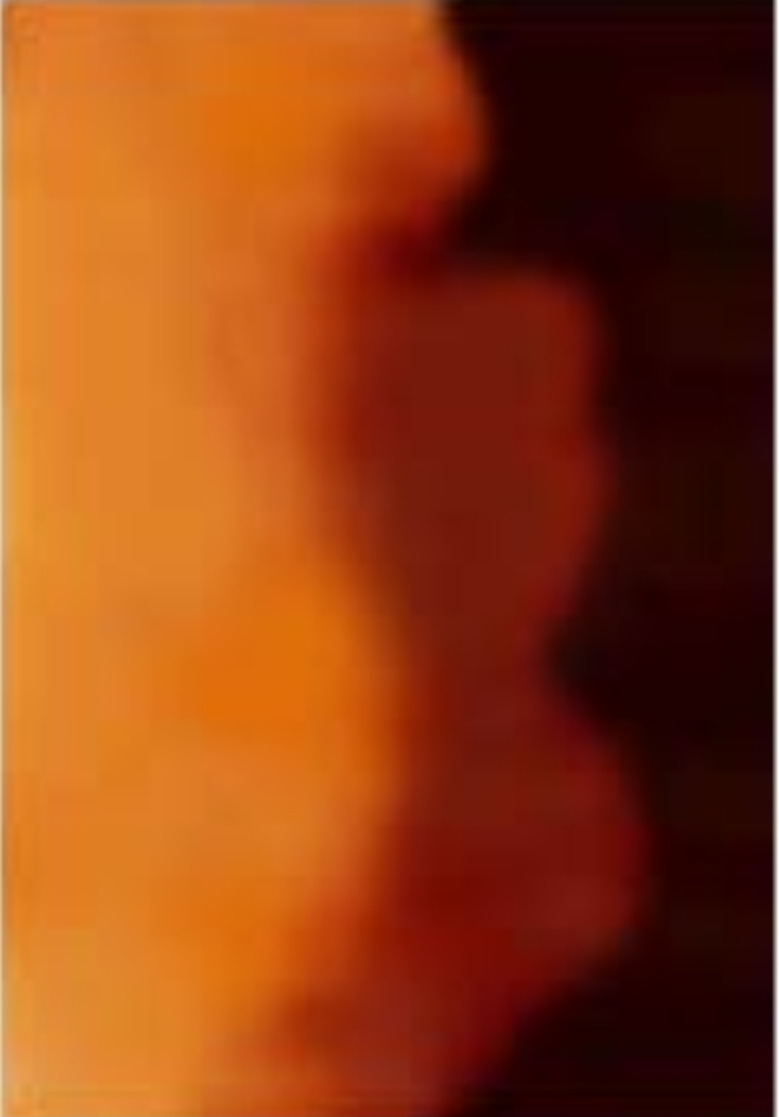
\includegraphics[width = 3.6cm]{Introduction/graphene.png}
\hspace{3cm}
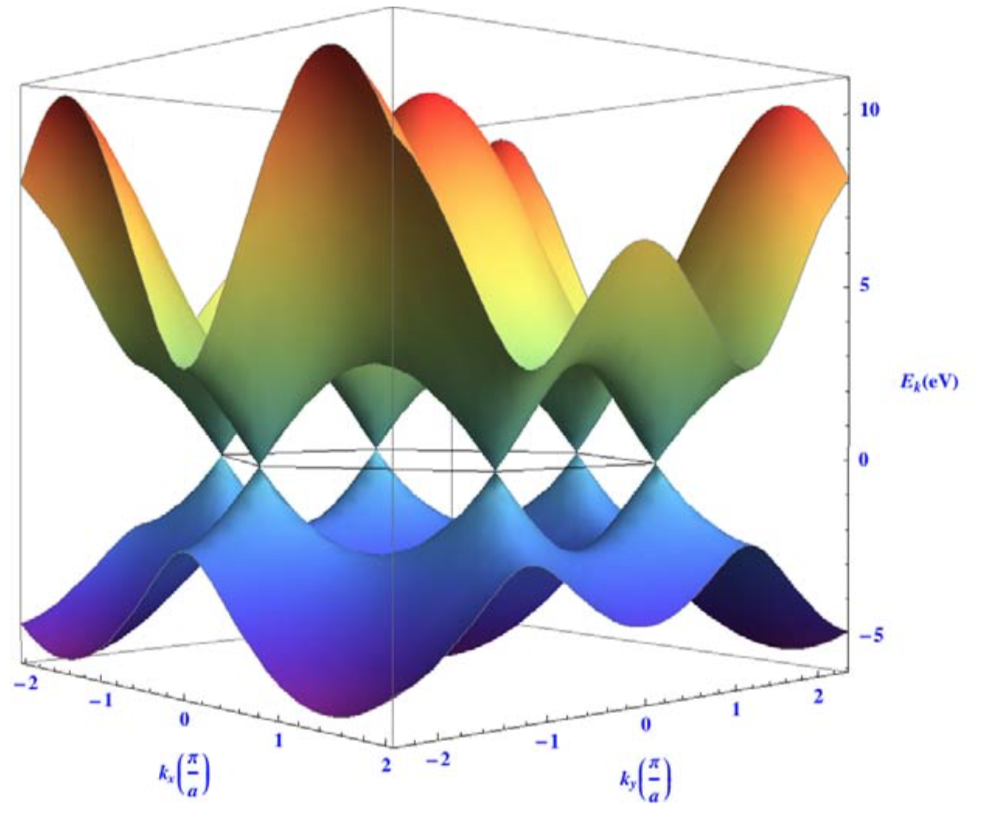
\includegraphics[width = 6.5cm]{Introduction/disp_rel.png}
\caption[Graphene monolayer; graphene's dispersion relation.]{Left: \acf{AFM} picture of a graphene monolayer. The black area is a substrate used for fabrication purposes. The dark orange area is a monolayer of graphene. Right: Dispersion relation of graphene. The black line represents the Fermi energy. Close to it, the dispersion relation is linear, corresponding to massless excitations (taken from \cite{noauthor_nobel_nodate}). }
\label{fig:graphene}
\end{figure}	

On the other hand, \acp{TMD} are a recent member of the \ac{2D} materials family \cite{wang_electronics_2012, roldan_electronic_2014, xu_spin_2014}.
\acp{TMD} have been attracting interest because they seem to overcome some of the drawbacks of graphene in technological applications.
For example, monolayer graphene is gapless, while its bilayer counterpart has only a tunable, but small gap of the order of a tenth of an $eV$.
Contrastingly, \acp{TMD} have an intrinsic gap in excess of $1 \, eV$, being more promising in designing, for example, transistors.
Hole-doped \acp{TMD} are expected to show topological superconductivity \cite{hsu_topological_2017}, while the superconducting phase of graphene has been predicted, but is not easily attained.
Superconductivity in graphene-like \ac{2D} materials is important because it could boost high speed nanoelectronics.
Moreover, the presence of transition metal atoms in \acp{TMD} suggests the possibility of magnetic ordering \cite{braz_valley_2017}, which could be very relevant in nanospintronics applications.
Both topological superconductivity and magnetic ordering arise due to the effect of strong electron correlations.
Thus, to investigate these properties of \acp{TMD} when performing simulations, we need a computational method that is robust enough to capture the effects of electron interactions.

A nanoribbon consists of a \ac{2D} layer that can be regarded as infinitely long on one direction, but not on the other (Figure \ref{fig:fabrication}), so that edge states become relevant, and can be controlled to yield interesting properties.
For simulation purposes, it is natural to assume translational invariance along the ribbon's longitudinal direction, and use \acp{PBC}.
On the other direction, we use \acp{OBC}, effectively considering zigzag edges (Figure \ref{fig:nanoribbons}, left).

\begin{figure}[H]
\centering
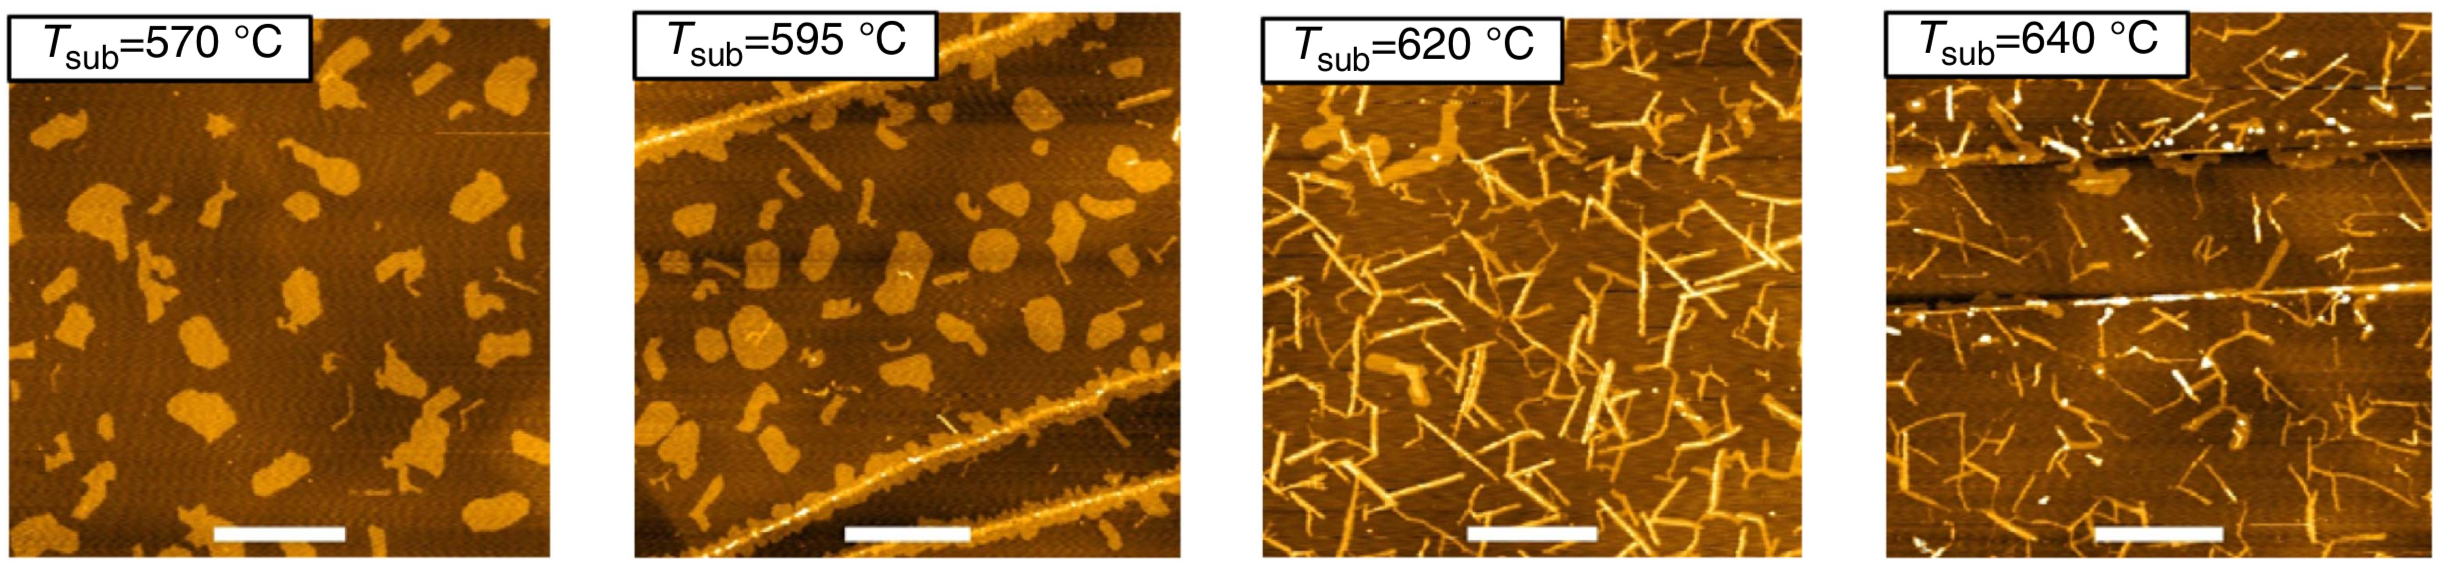
\includegraphics[scale = 0.35]{Introduction/nanoribbons}
\caption[Fabrication of \ac{TMD} nanoribbons]{Fabrication of \ac{TMD} nanoribbons. From left to right, we see \ac{AFM} images showing the appeareance of nanostructures ranging from \ac{2D} nanoislands to nanoribbons, as the temperature of the substrate is increased. The nanoribbons are grown by taking advantage of the temperature dependence of shape transformations occuring during the nonequilibrium growth of this kind of surface-based nanostructures. (taken from \cite{chen_fabrication_2017})}
\label{fig:fabrication}
\end{figure}
   
A high density of low-energy electronic states is localized at the zigzag edges, decaying quickly in the bulk, which suggests the possibility of magnetic ordering.
In fact, a mean field solution of the Hubbard model for a graphene nanoribbon shows that magnetic moments are localized at the edges \cite{yazyev_emergence_2010} (Figure \ref{fig:nanoribbons}, right).
QMC has been used to investigate edge-state magnetism beyond mean field in graphene \cite{feldner_dynamical_2011, golor_quantum_2013, cheng_strain-induced_2015, raczkowski_interplay_2017, yang_strain-tuning_2017}.
However, edge magnetism in TMD nanoribbons remains unexplored \cite{davelou_nanoribbon_2017}.
 
\begin{figure}[H]
\hspace{2cm}
\begin{minipage}[c]{0.1\textwidth}
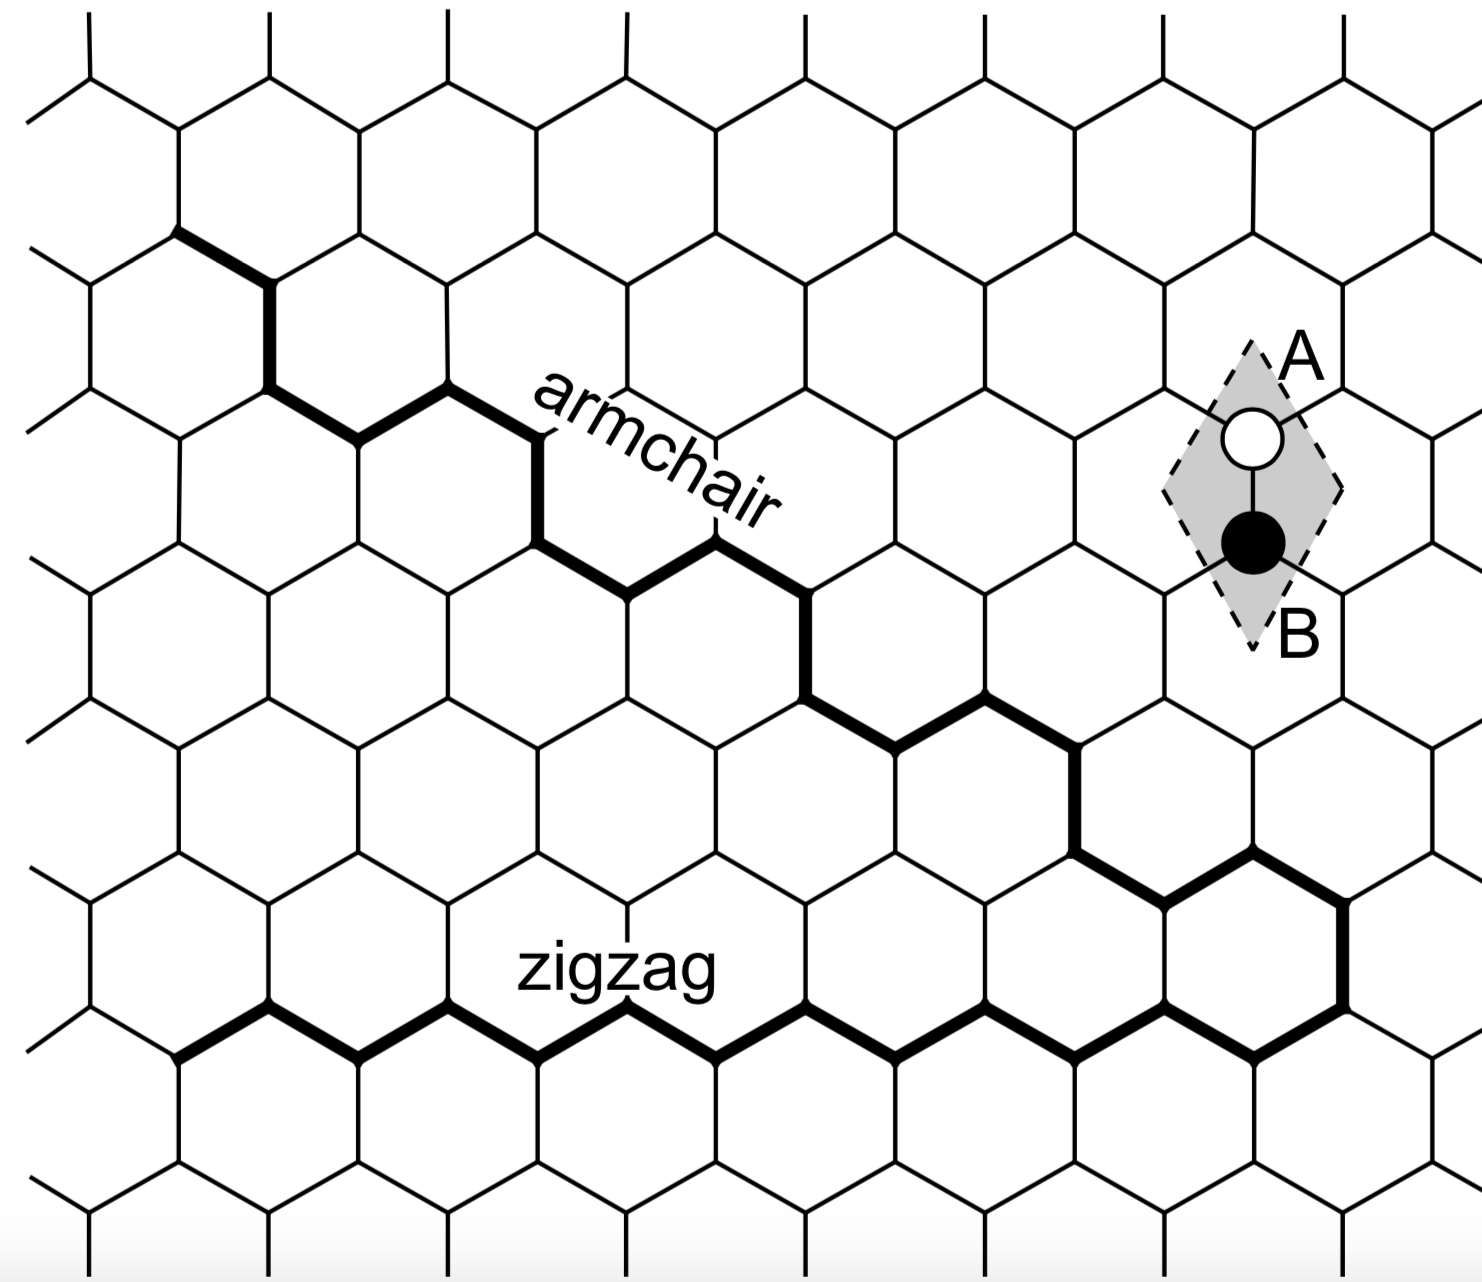
\includegraphics[scale = 0.22]{Introduction/zigzag}
\end{minipage} \hspace{6cm}
\begin{minipage}[c]{0.1\textwidth}
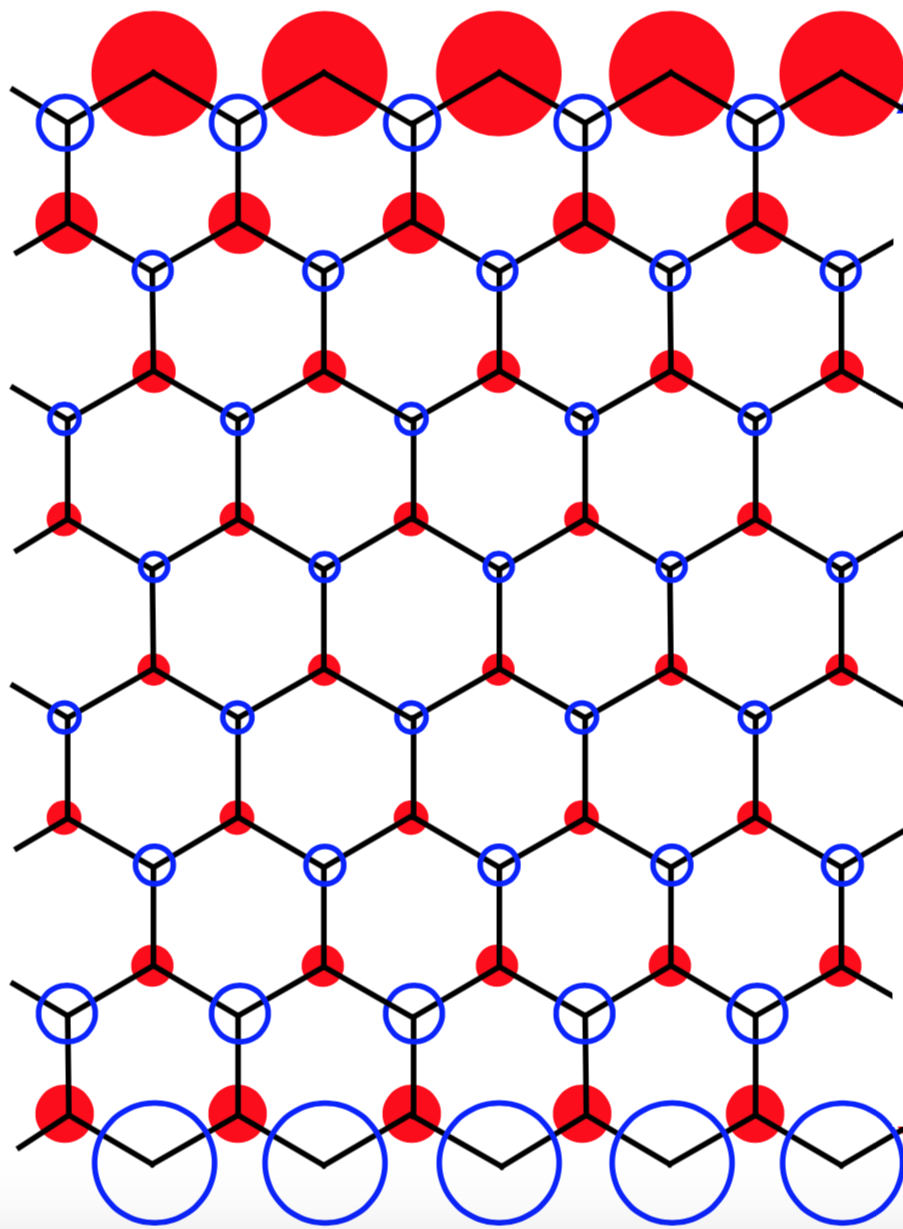
\includegraphics[scale = 0.23]{Introduction/edge_states}
\end{minipage}
 \caption[Zigzag edges of a nanoribbon and magnetism.]{Left: Two possible terminations of a \ac{TMD} nanoribbon condensing in a honeycomb lattice. Right: Local magnetic moments exist on the zig zag edges. The area of the circles corresponds to the magnitude of the magnetic moment, while the color red corresponds to a spin up density, and blue to a spin down density. The accumulation of electronic edge states leads to an \ac{AF} ground state (opposite edges with opposite magnetic moment). (taken from \cite{yazyev_emergence_2010}) \label{fig:nanoribbons}}
\end{figure}

While the zigzag graphene nanoribbon antiferromagnetic ground state is semiconducting, a state with interedge ferromagnetic orientation is a metal.
An example of an application based on the switching between the two states is a magnetorresistive sensor.
This device allows switching between low and high-resistance configurations, corresponding, respectively, to parallel, and antiparallel configurations of ferromagnetic leads at the ends of a nanoribbon.
An important application of this project is precisely the investigation of the possibility of edge-state magnetism, as is observed in graphene nanoribbons, for TMD nanoribbons, which could yield similarly innovative applications.


\subsection{Introduction to \acl{QMC}}

In principle, the properties of a quantum many-fermion system can all be deduced by solving an extremely complicated Schr\"odinger equation that takes into account the coupling of all (identical) particles of the system.
However, for the majority of systems the resulting integrals have no analytic solution, so we solve the problem by numerical integration.
But there is a myriad of methods to evaluate integrals numerically.
How do we pick the best one for this case? 
Multi-dimensional integrals are plagued by the curse of dimensionality.
Although the Newton-Cotes quadrature formulas (including, for example the Newton method, and Simpson's rules), Gaussian quadrature formulas, or Romberg's method all scale polynomially with the number of integration points, they become impractical as the dimension increases.
To use them, one would invoke Fubini's theorem to reduce the multi-dimensional integral to a series of one-dimensional integrals.
However, the number of function evaluations required to compute the whole integral grows exponentially with its dimension.
The Monte Carlo method preserves the polynomial scaling, thus yielding comparable accuracy with far less function evaluations.
It is natural to use it since typically the state space of our quantum system is huge, leading to high dimensional integrals.

The Monte Carlo method is ubiquitous.
Its central idea is to use randomness to produce accurate estimates of deterministic integrals.
The term was coined by Nicolas Metropolis in 1949, first appearing in a seminal paper, in which it was described as a \say{statistical approach to the study of differential equations, or more generally, of integro-differential equations that occur in various branches of sciences}\cite{metropolis_monte_1949}.
Although it was used as early as 1777 in an experiment known as Buffon's needle - where one obtains an estimate of the constant $\pi$ by repeatedly throwing a needle randomly onto a sheet of paper with evenly spaced lines - it was crucially developed in the Los Alamos National Laboratory during World War II where the development of the first atomic bomb was completed, the primary objective of the Manhattan Project.
The method is particularly useful when one wants to sample from a probability distribution in an exponentially large state space.
In fact, it can in principle be used to solve any problem allowing a probabilistic formulation.

A variety of \acf{QMC} methods exists, using a sampling scheme based on the Metropolis algorithm, and variations thereof.
Variational and Diffusion \ac{QMC} are the simplest \ac{QMC} methods that allow one to capture some properties of correlated systems.
Although they already contain the main concepts used in this type of simulations, it is not always possible to use them. 
We will discuss their flaws and show how further refinement leads to the determinant, or auxiliary field method we ultimately used.

Using the Monte Carlo approach to study a many-fermion system implies overcoming a significant obstacle common to all \ac{QMC} methods - the so called \emph{fermion-sign problem}.
Pauli's exclusion principle implies that the many-fermion wave function is anti-symmetric, which leads to a sign oscillation that greatly impedes the accurate evaluation of averages of quantum observables.
The anti-symmetry constraint implies that a  straightforward weight interpretation of the wave function is not possible.
In the case of the finite temperature algorithm, the cancellations that occur when computing the average of any physical observable lead to poor statistical properties of the corresponding estimators.
This means that a massive amount of samples requiring enormous computer time are needed to obtain meaningful results.
In the case of the zero temperature algorithms, the situation is even worse.
It might not even be possible to design a stochastic process carrying the system to its ground state, as normally is done in \say{projective} methods\footnote{Methods that iteratively project a trial wave function onto the ground state.}: the wave function that is used as an initial proposal turns out to converge to a bosonic one, and the fermionic character of the system is lost.

As was proven by Troyer, the \emph{fermion-sign problem} has NP\footnote{NP or nondeterministic polynomial time, meaning that one can devise an algorithm that verifies the "yes" answer to a decision problem in polynomial time in the system size.
Note that the class $P$ - of polynomial time algorithms - is a subclass of NP.} computational complexity \cite{troyer_computational_2005}.
One of the greatest open questions in computer science is whether $P = NP$.
Solving the \emph{fermion-sign problem} would imply finding a solution to $P = NP$, which would constitute a major breakthrough.



\subsection{Variational Monte Carlo}

Variational techniques rely on an educated guess for the wave function of the system.
One introduces a set of variational parameters $\bm \alpha$ that are then tuned according to a variational principle.
Then, we may use the optimized trial wave function to compute physical quantities of interest using Monte Carlo.
The method is used to obtain zero temperature properties of a given model.
Note that it requires prior knowledge about the system to propose an approximate wave function in the first place.

A particularly relevant observable is the variational energy $E_V$ associated to a trial ground state.
Let $\bm r$ be the $3N$ spatial coordinates of the $N$ electrons.
Given the Hamiltonian of the system $\mathcal{H}$, and a trial wave function $\psi (\bm r)$ - a guess of the wave function representing the ground state - one can compute the corresponding variational energy.

\begin{equation}\label{eq:variational_energy}
E_V = \frac{\left\langle \psi | \mathcal{H} | \psi \right \rangle}{\left\langle \psi | \psi \right \rangle} = \frac{ \int d\bm r |\psi (\bm r)|^2 E_L (\bm r)}{\int d\bm r | \psi (\bm r)|^2 } = \int d\bm r\rho (\bm r) E_L (\bm r) ,
\end{equation}
where the local energy $E_L (\bm r)$ is defined as

\begin{equation}\label{eq:local_energy}
E_L = \frac{\mathcal{H} \psi (\bm r) }{\psi (\bm r)}
\end{equation}
and the probability distribution $\rho (\bm r)$ is defined as

\begin{equation}\label{eq:rho}
\rho (\bm r) = \frac{ | \psi (\bm r) |^2}{ \int d\bm r' | \psi (\bm r') |^2}
\end{equation}

Note that we managed to recast the variational energy as an average of the \emph{local} energy, $\left\langle E_L \right\rangle $, over the the distribution $\rho$.
This may be computed using the Monte Carlo method by sampling $M$ points $\bm r_k$ from distribution $\rho (\bm r)$:

\begin{equation}\label{eq:average}
E_V \approx \overline{E}_L = \frac{1}{M} \sum_{k= 1}^{M} E_L (\bm r_k) ,
\end{equation}
where $\overline {X}$ denotes a sample mean of the random variable $X$.

Let the ground state energy be $E_0$.
Then, states are optimized according to the variational principle:

\begin{equation}
E_V(\bm \alpha) = \frac{\left\langle \psi_{\bm \alpha} | \mathcal{H} | \psi_{\bm \alpha} \right\rangle}{\left\langle\psi_{\bm \alpha} | \psi_{\bm \alpha} \right\rangle} \ge E_0,
\end{equation}
where $\psi_{\bm \alpha}$ is the trial ground state wave function for the set of variational parameters ${\bm \alpha}$.

By varying $\bm \alpha$ we aim to obtain a variational energy that is as close as possible to the true ground state energy.
Since $E_V(\bm \alpha)$ is bounded from below, this is equivalent to minimizing it in the hope that $E_V(\bm \alpha_{min}) \gtrsim E_0$, i.e. the bound is tight.

The finite sampling size $M$, of course, introduces a statistical error common to all Monte Carlo methods. 
However, the use of an approximate wave function introduces a systematic error that is hard to control since trial wave functions are generally introduced based on approximate, or heuristic arguments.

\subsection{Diffusion Monte Carlo and projective methods}\label{subsec:dmc}

Variational Monte Carlo is severely limited by the use of a trial wave function $\psi_{\bm \alpha} (\bm r)$ because we may even not have enough information to even construct a reliable variational wave function.

Diffusion \ac{QMC} allows the simulation of a many-body system while having only a limited knowledge of the system's physical properties.
While it is exact for many-boson systems, it is only approximate for many-fermion systems.
The idea is to map the Schr\"odinger equation into  an imaginary-time diffusion equation.
Excited states are then filtered out by a diffusion process as we advance in imaginary-time.
In imaginary-time $\tau = i t$, the solution to the Schr\"odinger equation in terms of a formal series expansion in the eigenfunctions of the hamiltonian becomes a series of transients $e^{-E_n \tau}, \, n \in \mathbb{N}$.
The longest lasting of these is the ground state  \cite{kosztin_introduction_1996}.

The idea of the diffusion method is to generate samples using the exact ground state wave function $\psi_0 (\bm r)$ \cite{toulouse_chapter_2016}.
The associated exact energy $E_0$ is the matrix element of the hamiltonian calculated using a trial wave function and the ground state wave function.

\begin{equation}
E_0 = \frac{ \left\langle \psi_0 |E_0 \mathbbm{1} | \psi \right\rangle}{\left\langle \psi_0 | \psi \right\rangle} = \frac{\left\langle \psi_0 | \mathcal{H} | \psi \right\rangle}{ \left\langle\psi_0 | \psi \right\rangle} = \frac{\int d\bm r \psi_0^\star (\bm r) \psi (\bm r) E_L (\bm r)}{\int d\bm r\psi_0^\star (\bm r) \psi (\bm r)}
\end{equation}

Note that using this trick we avoid the computation of $\mathcal{H} \psi_0 = E_0 \psi_0$, that is, the ground state energy.
Instead, we approximate the integral by considering $M$ configuration samples $\bm r_{k = 1,..., N}$ in a similar spirit to that of Variational \ac{QMC}.
Notice that the integral consists of a local energy of the trial wave function $E_L (\bm r) = \frac{\mathcal{H} \psi (\bm r)}{\psi (\bm r)}$ averaged over a mixed distribution from which we draw a sample of points $\bm r_{k=1,...M}$:

\begin{equation}
f(\bm r) = \frac{\psi_0^\star (\bm r) \psi (\bm r) }{ \int d\bm r  \psi_0 (\bm r) \psi (\bm r)}
\end{equation}

Although the method is, of course, aimed at probing many-body systems, let us consider a single particle in \acs{1D} for simplicity for illustrating the method.
Performing a Wick rotation - effectively going to imaginary time - and shifting the energy, the Schr\"odinger equation becomes

\begin{equation}
\frac{\partial \psi ( x, \tau )}{\partial\tau}  = -\frac{1}{2m}\frac{\partial^2 \psi ( x, \tau )}{\partial x^2} - \bigg[ V(x) - E_T \bigg] \psi( x, \tau ) 
\end{equation}

The exact ground state wave function $\psi_0 ( x )$ is obtained as the longest lasting transient state in imaginary time: we are interested in the asymptotic behavior of the series expansion constituting the formal solution of the Schr\"odinger equation

\begin{equation}
\psi (x, \tau) = \sum_{n=0}^{\infty} c_n \psi_n (x) e^{-(E_n - E_T)\tau}
\end{equation}

Imaginary time evolution is governed by

\begin{equation}\label{eq:im_ev}
\begin{split}
&\left| \psi (t) \right\rangle = \lim_{\tau \rightarrow \infty} \sum_i e^{-(E_i - E_T) \tau} \left|\psi_i \right\rangle \left\langle \psi_i | \psi \right\rangle = \\
&= \lim_{\tau \rightarrow \infty} e^{-(E_0 - E_T)\tau} \left| \psi_0 \right\rangle \left\langle \psi_0 | \psi \right\rangle 
\end{split}
\end{equation}


If $E_T > E_0$ the wave function diverges exponentially fast: $\lim_{\tau \rightarrow \infty} \psi ( x, \tau) = \infty$.
Similarly, for $E_T < E_0$ it vanishes exponentially fast: $\lim_{\tau \rightarrow \infty} \psi ( x, \tau) = 0$.
However, if $E_T = E_0$ the wave function converges to the ground state one up to a constant factor.

\begin{equation}\label{eq:dmc}
\lim_{\tau \rightarrow \infty} \psi ( x, \tau) = c_0 \psi_0 (x) \,\,\, \text{, or} \quad \lim_{\tau \rightarrow \infty} \left|\psi (\tau) \right\rangle \propto \left| \psi_0 \right\rangle
\end{equation}

Diffusion \ac{QMC} makes use of Eq. (\ref{eq:dmc}), approximating $\psi_0(x)$ by $\psi (x, \tau)$ for sufficiently long time.
The only requirement is that $\psi (x, \tau)$ and $\psi_0(x)$ overlap significantly so that $c_0$ is large enough to be numerically measurable, and we can always center a positive trial wave function in a region where $\psi_0(x)$ is large enough and positive.
If the latter condition does not hold, the wave function converges to a bosonic, instead of a fermionic one.
Of course, these conditions can always be met for a single particle, but note that they might fail for a many-fermion system, for which the wave function crosses a number of nodes due to its anti-symmetric nature.

\subsection{Drawbacks of variational and projective methods. Auxiliary Field \acs{QMC}. The Fermion Sign Problem.}
\label{subsec:introAFQMC}

As we have seen, the major drawback of the variational method was that it demanded \emph{a priori} knowledge of a reasonable variational wave function describing, at least partly, some of the physics of the problem.
Diffusion \acs{QMC} demands less: we need only propose a trial wave function that overlaps with the ground state.
However, none of these methods allow us to probe systems at finite temperature.
Moreover, they both require some prior knowledge about the system, which may not always be available.

An alternative method is based on introducing an additional lattice bosonic field that mediates the electron-electron interaction.
The interacting problem then becomes a problem of independent fermions coupled to an external field, and the fermionic part of the partition function can be traced out explicitly, leaving the contribution of a \emph{discrete}\footnote{Although, there is a finite number of field configurations, the number grows exponentially with the number of sites on the lattice.} bosonic field.
This contribution can be evaluated numerically by employing importance sampling over the field configurations.
Auxiliary field \acs{QMC} relies on a mapping to a classical system:

\begin{equation}
Z = \Tr [ e^{-\beta \mathcal{H} } ] = \sum_c p_c ,
\end{equation}
but some of the \say{probabilities} can actually be negative $p_c < 0$.
This occurs due to the antisymmetry of the many-electron wave function under exchange of two electrons.

The negative weight problem may easily be circumvented when computing averages of observables:

\begin{equation}\label{eq:signSampling}
\left\langle A \right\rangle = \frac{\sum_c A ( c ) p ( c )}{\sum_c p ( c ) } = \frac{\sum_c A ( c )|  p ( c ) | \text{sign}[p(c)] / \sum_c | p ( c ) | }{\sum_c  |  p ( c ) | \text{sign}[p(c)] /  \sum_c | p ( c ) |} \equiv \frac{\left\langle A s \right\rangle_{|p|}}{\left\langle s \right\rangle_{|p|}} ,
\end{equation}
where $s(c) = \text{sign} [ p ( c ) ]$, and $| p ( c ) | $ corresponds to an auxiliary bosonic system (also coupled to the bosonic field) corresponding to the original fermionic system, and for which there is no sign problem.

The relative error $\Delta s / \left\langle s \right\rangle$ increases exponentially with the number of particles, with inverse temperature, and possibly with other parameters of the specific model to be studied \cite{troyer_computational_2005, hou_numerical_2009}.
To see this, we start by noting that the average sign is the ratio between the partition functions of the fermionic ($Z = \sum_c p(c)$) and bosonic systems ($Z = \sum_c | p ( c ) |$).
In terms of the difference in free energy densities, $\left\langle s \right\rangle = Z / Z' = e^{-\beta N_p \Delta f}$, implying that for $M$ samples, the error of the denominator of Eq. (\ref{eq:signSampling}) becomes

\begin{equation}
\frac{\Delta s}{\left\langle s \right\rangle} = \frac{\sqrt{(\left\langle s^2 \right\rangle - \left\langle s \right\rangle^2 )/ M }}{\left\langle s \right\rangle} = \frac{ \sqrt{ 1 - \left\langle s \right\rangle^2}  }{\sqrt{M} \left\langle s \right\rangle} \propto \frac{e^{\beta N_p \Delta f}}{\sqrt{M}} ,
\end{equation}
and similarly for the numerator of Eq. (\ref{eq:signSampling}).

Auxiliary field \acs{QMC} can also be formulated to probe ground state properties, and a sign problem arises similarly.
Apart from this problem, which plagues all \acs{QMC} methods, this method is one of the most robust, unbiased, and reliable methods, hence we choose it to carry out our simulations.
Note that, in particular, it is certainly more powerful than the variational and diffusion methods outlined before since it requires much less \emph{a priori} information about the system.
Perhaps more importantly, given some recent findings, it can be used in conjunction with neural networks to discover quantum phase transitions in correlated systems  \cite{broecker_machine_2017}.
\section{Introduction to \acl{QMC}}
\label{sec:introQMC}

Solving the many-body problem remains one of the greatest challenges in physics.
Following the wealth of attempts at such pursuit, certain phenomena arising due to the strong interactions in quantum systems are explained in different theoretical frameworks, namely superconductivity, the Mott metal-insulator transition, and fractional quantum Hall effect.
All of these breakthroughs represented revolutions in their respective fields with significant scientific and technological impact.
However, only in very limited cases does an actual analytical solution exist for the  Schr\"odinger equation for a system of interacting particles.
One must resort to sophisticated approximation methods to obtain  information about the role played by the competing interactions under various conditions in the aforementioned cases.
It is then natural that numerical methods have become prominent as a tool for extracting useful information about this type of systems.
\ac{QMC} is amongst the most accurate and extensively studied ones.
The idea of all \ac{QMC} methods is to reduce the interacting problem to solving a set of integrals, which can be evaluated numerically through a standard stochastic procedure.
These integrals are arrived at upon formulating the quantum many-body description of the system using the Schr\"odinger equation.
Hence the name \acl{QMC}, which is used to distinguish it from Classical Monte Carlo.
In the classical version, one measures thermal averages, while in the quantum version, one measures expectations of operators over the Hilbert space of the system, corresponding to physical observables that fluctuate with a dynamics given by the Schr\"odinger equation (and, of course, can also have thermal fluctuations).
In fact, the dynamics of a quantum system are encoded in the Hamiltonian operator.
In the case of graphene-like \ac{2D} materials, one usually uses a tight-binding model.
It is found that the dynamics given by the tight-binding Hamiltonian is sufficient to describe most properties of graphene.
However, in other materials, such as \acp{TMD}, electron-electron interactions are stronger, and Hubbard-type models could give us a more accurate picture of the phenomena that occur within them.

For quantum many-fermion systems, observables are given in terms of integrals which have no analytic solution, so we solve the problem numerically.
But there is a myriad of methods to evaluate integrals numerically.
How do we pick the best one for this case? 
Multi-dimensional integrals are plagued by the curse of dimensionality.
Although the Newton-Cotes quadrature formulas (including, for example the Newton method, and Simpson's rules), Gaussian quadrature formulas, or Romberg's method all scale polynomially with the number of integration points, they become impractical as the dimension increases.
To use them, one would invoke Fubini's theorem to reduce the multi-dimensional integral to a series of one-dimensional integrals.
However, the number of function evaluations required to compute the whole integral grows exponentially with its dimension.
The Monte Carlo method preserves the polynomial scaling, thus yielding comparable accuracy with far less function evaluations.
It is natural to use it since typically the state space of our quantum system is huge, leading to high dimensional integrals.

The Monte Carlo method is ubiquitous.
Its central idea is to use randomness to produce accurate estimates of deterministic integrals.
The term was coined by Metropolis in 1949, although it was used as early as 1777 in an experiment known as Buffon's needle - where one obtains an estimate of the constant $\pi$ by repeatedly throwing a needle randomly onto a sheet of paper with evenly spaced lines. %t was crucially developed in the Los Alamos National Laboratory during World War II where the development of the first atomic bomb was completed, the primary objective of the Manhattan Project.
The method is particularly useful when one wants to sample from a probability distribution in an exponentially large state space (like the huge Hilbert space of an interacting electron system), but it can, in principle, be used to solve any problem allowing a probabilistic formulation.
To solve the interacting fermion problem, a variety of \ac{QMC} methods exists, using a sampling scheme based on the Metropolis algorithm, and variations thereof.
Variational and Diffusion \ac{QMC} are the simplest \ac{QMC} methods that allow one to capture some properties of correlated systems, but it is not always ideal or even possible to use them. 
%We will discuss their flaws and show how further refinement leads to the auxiliary field method we ultimately used.

Using the Monte Carlo approach to study a many-fermion system implies overcoming a significant obstacle common to all \ac{QMC} methods - the so called \emph{fermion sign problem}.
Pauli's exclusion principle implies that the many-fermion wave function is anti-symmetric, which leads to a sign oscillation that greatly impedes the accurate evaluation of averages of quantum observables.
The anti-symmetry constraint implies that a  straightforward weight interpretation of the wave function is not possible.
In the case of the finite temperature algorithm, the cancellations that occur when computing the average of any physical observable lead to poor statistical properties of the corresponding estimators.
This means that a massive amount of samples requiring enormous computer time are needed to obtain meaningful results.
In the case of the zero temperature algorithms, the situation is even worse.
It might not even be possible to design a stochastic process carrying the system to its ground state, as normally is done in \say{projective} methods\footnote{Methods that iteratively project a trial wave function onto the ground state.}: the wave function that is used as an initial proposal turns out to converge to a bosonic one, and the fermionic character of the system is lost.
As was proven by Troyer, the \emph{fermion sign problem} has NP\footnote{NP or nondeterministic polynomial time, meaning that one can devise an algorithm that verifies the "yes" answer to a decision problem in polynomial time in the system size.
Note that the class $P$ - of polynomial time algorithms - is a subclass of NP.} computational complexity \cite{troyer_computational_2005}.
One of the greatest open questions in computer science is whether $P = NP$.
Solving the \emph{fermion sign problem} would imply finding a solution to $P = NP$, which would constitute a major breakthrough.

\subsection{Variational Monte Carlo}

Variational techniques rely on an educated guess for the wave function of the system.
One introduces a set of variational parameters $\bm \alpha$ that are then tuned according to a variational principle.
Then, we may use the optimized trial wave function to compute physical quantities of interest using Monte Carlo.
The method is used to obtain zero temperature properties of a given model.
Note that it requires prior knowledge about the system to propose an approximate wave function in the first place.

A particularly relevant observable is the variational energy $E_V$ associated to a trial ground state.
Let $\bm r$ be the $3N$ spatial coordinates of the $N$ electrons.
For simplicity, let us ignore all other degrees of freedom, such as spin.
Given the Hamiltonian of the system $\mathcal{H}$, and a trial wave function $\psi_T (\bm r)$ - a guess of the wave function representing the ground state - one can compute the corresponding variational energy by averaging over a \say{local} energy:

\begin{equation}\label{eq:variational_energy}
E_V = \frac{\left\langle \psi_T | \mathcal{H} | \psi_T \right \rangle}{\left\langle \psi_T | \psi_T \right \rangle} = \frac{ \int d\bm r |\psi_T (\bm r)|^2 E_L (\bm r)}{\int d\bm r | \psi_T (\bm r)|^2 } = \int d\bm r\rho (\bm r) E_L (\bm r) , \text{where}
\end{equation}

\begin{equation}\label{eq:local_energy}
E_L = \frac{\mathcal{H} \psi_T (\bm r) }{\psi_T (\bm r)}   \quad \text{and} \quad \rho (\bm r) = \frac{ | \psi_T (\bm r) |^2}{ \int d\bm r' | \psi_T (\bm r') |^2}
\end{equation}

Note that we managed to recast the variational energy as an average of the \emph{local} energy, $\left\langle E_L \right\rangle $, over the the distribution $\rho$.
This may be computed using the Monte Carlo method by sampling $M$ points $\bm r_k$ from the distribution $\rho (\bm r)$.
Denoting the sample mean of the random variable $X$ as $\overline {X}$:

\begin{equation}\label{eq:average}
E_V \approx \overline{E}_L = \frac{1}{M} \sum_{k= 1}^{M} E_L (\bm r_k) ,
\end{equation}

Let the ground state energy be $E_0$.
Then, states are optimized according to the variational principle:

\begin{equation}
E_V(\bm \alpha) = \frac{\left\langle \psi_{\bm \alpha} | \mathcal{H} | \psi_{\bm \alpha} \right\rangle}{\left\langle\psi_{\bm \alpha} | \psi_{\bm \alpha} \right\rangle} \ge E_0,
\end{equation}
where $\psi_{\bm \alpha}$ is the trial ground state wave function for the set of variational parameters ${\bm \alpha}$.
By varying $\bm \alpha$ we aim to obtain a variational energy that is as close as possible to the true ground state energy, and use the corresponding trial wave function to compute averages of other observables.
Since $E_V(\bm \alpha)$ is bounded from below, this is equivalent to minimizing it in the hope that $E_V(\bm \alpha_{min}) \gtrsim E_0$, i.e. the bound is tight.
The finite sampling size $M$, of course, introduces a statistical error common to all Monte Carlo methods. 
However, the use of an approximate wave function introduces a systematic error that is hard to control since trial wave functions are generally introduced based on approximate, or heuristic arguments.

\subsection{Diffusion Monte Carlo and projective methods}\label{subsec:dmc}

Variational Monte Carlo is severely limited by the use of a trial wave function $\psi_T (\bm r)$ because we may not even have enough information to even construct a reliable variational wave function in the first place.
Diffusion \ac{QMC} allows the simulation of a many-body system while having only a limited knowledge of the system's physical properties.
As a projective method, it is exact for many-boson systems, while being only approximate for many-fermion systems.
The idea is to map the Schr\"odinger equation onto an imaginary-time diffusion equation.
Excited states are then filtered out by a diffusion process as we advance in imaginary-time.
In imaginary-time $\tau = i t$, the solution to the Schr\"odinger equation in terms of a formal series expansion in the eigenfunctions of the Hamiltonian becomes a series of \say{transient} wavefunctions weighted by $e^{-E_n \tau}, \, n \in \mathbb{N}$.
Within precision and accuracy constraints, the longest lasting of these is the ground state \cite{kosztin_introduction_1996}.
Thus, the idea of the diffusion method is to generate samples using the exact ground state wave function $\psi_0 (\bm r)$ \cite{toulouse_chapter_2016}.
The associated exact energy $E_0$ is the matrix element of the hamiltonian calculated using a trial wave function and the ground state.

\begin{equation}
E_0 = \frac{ \big( \left\langle \psi_0 |E_0 \big) \big( \mathbbm{1} | \psi_T \right\rangle \big)}{\left\langle \psi_0 | \psi_T \right\rangle} = \frac{\left\langle \psi_0 | \mathcal{H} | \psi_T \right\rangle}{ \left\langle\psi_0 | \psi_T \right\rangle} = \frac{\int d\bm r \psi_0^\star (\bm r) \psi_T (\bm r) E_L (\bm r)}{\int d\bm r\psi_0^\star (\bm r) \psi_T (\bm r)}
\end{equation}

Note that using this trick we avoid the computation of $\mathcal{H} \psi_0 = E_0 \psi_0$, that is, the ground state energy.
Instead, we approximate the integral by considering $M$ configuration samples $\bm r_{k = 1,..., M}$ in a similar spirit to that of Variational \ac{QMC}.
Notice that the integral consists of a local energy of the trial wave function $E_L (\bm r) = \frac{\mathcal{H} \psi (\bm r)}{\psi (\bm r)}$ averaged over a mixed distribution from which we draw a sample:

\begin{equation}
f(\bm r) = \frac{\psi_0^\star (\bm r) \psi_T (\bm r) }{ \int d\bm r  \psi_0 (\bm r) \psi_T (\bm r)}
\end{equation}

Although the method is, of course, aimed at probing many-body systems, let us consider a single particle in \acs{1D}, for simplicity, to illustrate the method.
Performing a Wick rotation - effectively going to imaginary time - and shifting the energy, the Schr\"odinger equation becomes (with $\hbar = 1$)

\begin{equation}
\frac{\partial \psi_T ( x, \tau )}{\partial\tau}  = -\frac{1}{2m}\frac{\partial^2 \psi_T ( x, \tau )}{\partial x^2} - \bigg[ V(x) - E_T \bigg] \psi_T( x, \tau ) 
\end{equation}

The exact ground state wave function $\psi_0 ( x )$ is obtained as the longest lasting transient state in imaginary time: we are interested in the asymptotic behavior of the series expansion constituting the formal solution of the Schr\"odinger equation

\begin{equation}
\psi_T (x, \tau) = \sum_{n=0}^{\infty} c_n \psi_n (x) e^{-(E_n - E_T)\tau}
\end{equation}

Imaginary time evolution is governed by

\begin{equation}\label{eq:im_ev}
\left| \psi_T (t) \right\rangle = \lim_{\tau \rightarrow \infty} \sum_n e^{-(E_n - E_T) \tau} \left|\psi_n \right\rangle \left\langle \psi_n | \psi_T \right\rangle = \lim_{\tau \rightarrow \infty} e^{-(E_0 - E_T)\tau} \left| \psi_0 \right\rangle \left\langle \psi_0 | \psi_T \right\rangle 
\end{equation}

If $E_T > E_0$ the wave function diverges exponentially fast: $\lim_{\tau \rightarrow \infty} \psi_T ( x, \tau) = \infty$.
Similarly, for $E_T < E_0$ it vanishes exponentially fast: $\lim_{\tau \rightarrow \infty} \psi_T ( x, \tau) = 0$.
However, if $E_T = E_0$ the wave function converges to the ground state one up to a constant factor, $c_0 = \left\langle \psi_0 | \psi_T \right\rangle$.

\begin{equation}\label{eq:dmc}
\lim_{\tau \rightarrow \infty} \psi_T ( x, \tau) = c_0 \psi_0 (x) \quad \text{or} \quad \lim_{\tau \rightarrow \infty} \left|\psi_T (\tau) \right\rangle \propto \left| \psi_0 \right\rangle
\end{equation}

Diffusion \ac{QMC} makes use of Eq. (\ref{eq:dmc}), approximating $\psi_0(x)$ by $\psi_T (x, \tau)$ for sufficiently long time.
The only requirement is that $\psi_T (x, \tau)$ and $\psi_0(x)$ overlap significantly so that $c_0$ is large enough to be numerically measurable, and we can always center a positive trial wave function in a region where $\psi_0(x)$ is large enough and positive.
If the latter condition does not hold, the wave function converges to a bosonic, instead of a fermionic one.
Of course, these conditions can always be met for a single particle, but note that they might fail for a many-fermion system, for which the wave function crosses a number of nodes due to its anti-symmetric nature.

\subsection{Auxiliary Field \acs{QMC} and the Fermion Sign Problem}
\label{subsec:introAFQMC}

As we have seen, the major drawback of the variational method was that it demanded \emph{a priori} knowledge of a reasonable variational wave function describing, at least partly, some of the physics of the problem.
Diffusion \acs{QMC} demands less: we need only propose a trial wave function that overlaps with the ground state.
However, none of these methods allow us to probe systems at finite temperature.
Moreover, they both require some prior knowledge about the system, which may not always be available.

An alternative method is based on introducing an additional lattice bosonic field that mediates the electron-electron interaction.
The interacting problem then becomes a problem of independent fermions coupled to an external field, and the fermionic part of the partition function can be traced out explicitly, leaving the contribution of a \emph{discrete}\footnote{The introduced field is discrete (and \emph{binary}) because each fermionic state can only have occupations $n = 0, 1$. Although, there is a finite number of field configurations, the number grows exponentially with the number of sites on the lattice.} bosonic field, $\bm h$.
This contribution can be evaluated numerically by employing importance sampling over the field configurations.
Auxiliary field \acs{QMC} relies on a mapping to a so called \say{classical} system (in quotes because there may be no actual classical analogue):

\begin{equation}\label{eq:Zsign}
Z = \Tr [ e^{-\beta \mathcal{H} } ] = \sum_{\{ \bm h\} } \sum_{\text{fermionic}} e^{-S} = \sum_c p_c ,
\end{equation}
but some of the \say{probabilities} can actually be negative $p_c < 0$.
This occurs due to the antisymmetry of the many-electron wavefunction under electron exchange, and is at the root of the sign problem.
Here, $S$ is a fermion-boson action that we shall write out explicitly later.
For a fixed configuration of the bosonic field, we sum over the fermionic part exactly to obtain the weight of each configuration $p_c$.
The sum over $\bm h$ is carried out stochastically.

The negative weight problem may easily be circumvented when computing averages of observables:

\begin{equation}\label{eq:signSampling}
\left\langle A \right\rangle = \frac{\sum_c A ( c ) p ( c )}{\sum_c p ( c ) } = \frac{\sum_c A ( c )|  p ( c ) | \text{sign}[p(c)] / \sum_c | p ( c ) | }{\sum_c  |  p ( c ) | \text{sign}[p(c)] /  \sum_c | p ( c ) |} \equiv \frac{\left\langle A s \right\rangle_{|p|}}{\left\langle s \right\rangle_{|p|}} ,
\end{equation}
where $s(c) = \text{sign} [ p ( c ) ]$, and $| p ( c ) | $ corresponds to an auxiliary bosonic system (also coupled to the bosonic field) corresponding to the original fermionic system, and for which there is no sign problem.

The relative error $\Delta s / \left\langle s \right\rangle$ increases exponentially with the number of particles, with inverse temperature, and possibly with other parameters of the specific model to be studied \cite{troyer_computational_2005, hou_numerical_2009}.
To see this, we start by noting that the average sign is the ratio between the partition functions of the fermionic ($Z = \sum_c p(c)$) and bosonic systems ($Z' = \sum_c | p ( c ) |$).
In terms of the difference in free energy densities, $\left\langle s \right\rangle = Z / Z' = e^{-\beta N_p \Delta f}$, implying that for $M$ samples, the error of the denominator of Eq. (\ref{eq:signSampling}) becomes

\begin{equation}
\frac{\Delta s}{\left\langle s \right\rangle} = \frac{\sqrt{(\left\langle s^2 \right\rangle - \left\langle s \right\rangle^2 )/ M }}{\left\langle s \right\rangle} = \frac{ \sqrt{ 1 - \left\langle s \right\rangle^2}  }{\sqrt{M} \left\langle s \right\rangle} \propto \frac{e^{\beta N_p \Delta f}}{\sqrt{M}} ,
\end{equation}
and similarly for the numerator of Eq. (\ref{eq:signSampling}).

Auxiliary field, or determinant \acs{QMC} can also be formulated to probe ground state properties, and a sign problem arises similarly.
In fact, this problem plagues all \acs{QMC} methods, even though we showed it only for the determinant method\footnote{So called because, as we shall show later, $p_c$ boils down to a product of determinants that depends on the energy scales of the problem.}.
The latter is the most robust, unbiased, and reliable method, with a generally modest sign problem, hence we choose it to carry out our simulations.

Furthermore, in general, it suffices to use the finite temperature auxiliary field  method with $\beta$ large enough to probe ground state properties (for example, this is shown numerically for the Hubbard model on the square lattice in \cite{white_numerical_1989}).
In this case, the inverse temperature may be regarded as being analogous to a  projective parameter $\Theta$, characterizing convergence to the ground state, within statistical uncertainty.
Projector \ac{QMC}, the zero temperature version of auxiliary field \ac{QMC} is based on an equation similar to Eq.(\ref{eq:dmc}).
Any observable $A$ is computed by use of a trial wave function with some overlap with the ground state $\left\langle \psi_T | \psi_0 \right\rangle \neq 0$ (see \cite{f._assaad_quantum_2002} for more details on the projector method; in this work we focus on the finite temperature version since it is more general):

\begin{equation}
\left\langle A \right\rangle = \lim_{\Theta \rightarrow \infty} \frac{\left\langle \psi_T | e^{-\Theta \mathcal{H} } A e^{-\Theta \mathcal{H} } | \psi_T \right\rangle }{\left\langle \psi_T | e^{- 2 \Theta \mathcal{H} } | \psi_T \right\rangle}
\end{equation}

Note that auxiliary field \ac{QMC} is more powerful than the variational and diffusion methods outlined before since it requires much less \emph{a priori} information about the system.
Perhaps more importantly, recent work suggests that it can be used in conjunction with neural networks to discover quantum phase transitions in correlated systems  \cite{broecker_machine_2017} in what could be a revolution in the field.
\section{Original Contributions}
\label{sec:int_contributions}

In this work we focus mainly on the study of the magnetic properties of \ac{TMD} nanoribbons.
We compare our \ac{QMC} results with those obtained in the mean field approximation and benchmark them  against existing, \say{tried and true}  implementations (namely \texttt{ALF} \cite{bercx_alf_2017} and \texttt{QUEST} \cite{noauthor_quest_2012}), and early seminal studies \cite{hirsch_discrete_1983,white_numerical_1989}.

To carry out this study, we use \texttt{QUEST} and our own original implementation of the auxiliary field \ac{QMC} algorithm in \texttt{C++}.
The code we wrote can be used to simulate low-dimensional Hubbard-like models with different geometries to extend this work.
Additionaly, using our code, we characterize and compare different options to stabilize the matrix products needed to perform the simulations.
Lastly, we give a contribution to circumvent the fermion sign problem in an attempt to extract the maximum amount of information out of the Monte Carlo measurements.
\section{Outline}
\label{sec:int_outline}

We started this introductory chapter with the concept of emergence in strongly correlated electron systems.
Then, we proceeded to discuss the particular example we study in this thesis: the \acs{2D} \acs{TMD} nanoribbon.
In this system, we show that electron correlations give rise to emergent edge-state magnetism, which was unexplored numerically  before this work.
To tackle this interacting fermion system, we resort to a state-of-the-art determinant  \ac{QMC} algorithm.

In chapter (\ref{cap:hubbard}), we introduce the Hubbard model, a ubiquitous model of electron correlations.
We discuss analytical solutions of simple limiting cases, outline some approximation methods, and introduce Green's functions, which turn out to be the main object of our simulations.
Moreover, we formulate the mean field theory of the Hubbard model.
Then, we proceed to the simulation method.
In chapter (\ref{cap:afqmc}), we start by summarizing the main ideas about how to apply the Monte Carlo method to statistical physics problems.
In this context, we use original results of our simulations to illustrate the concepts in the specific context of our problem.
Still in chapter (\ref{cap:afqmc}), we introduce the auxiliary field method, and its various challenges, namely low temperature, and large size stabilization.

In chapter (\ref{cap:applications}), we apply the code we implemented for a variety of systems, benchmarking our code, and carrying out some original calculations both at the mean field level and using \acs{QMC} for \acp{TMD}.
Finally, in chapter (\ref{cap:conclusions}), we conclude by discussing the results obtained in the previous chapter in the context of the literature, and propose future work to be done on the topic.

\cleardoublepage
% %%%%%%%%%%%%%%%%%%%%%%%%%%%%%%%%%%%%%%%%%%%%%%%%%%%%%%%%%%%%%%%%%%%%%%
% The Introduction:
% %%%%%%%%%%%%%%%%%%%%%%%%%%%%%%%%%%%%%%%%%%%%%%%%%%%%%%%%%%%%%%%%%%%%%%
\fancychapter{Conclusions and Future Work}
\label{cap:conclusions}

Conclusions Chapter

\cleardoublepage
\cleardoublepage
\phantomsection 
\addcontentsline{toc}{chapter}{Bibliography}

\printbibliography

\cleardoublepage

\begin{appendices}
	\begin{appendix}
		\pagenumbering{bychapter}
		\chapter{Obtaining the Hubbard Model. Approximate Solutions}
\label{ap:hubbardObSol}

%\pagebreak

\section{Hartree-Fock Approximation and the Self Consistent Field}\label{sec:hartree-fock}

In the mean field approximation, the quartic term of the interaction part of the Hamiltonian
\begin{equation*}
V_{\text{int}} = \frac{1}{2} V^{\nu\mu}_{\nu'\mu'} c_\nu^\dagger c_\mu^\dagger c_{\mu'} c_{\nu'} ,
\end{equation*} 
becomes a sum of all possible 2-body terms (note that terms of the type $\left\langle cc \right\rangle$ and $\left\langle c^\dagger c^\dagger \right\rangle$ must vanish since they do not conserve the number of particles).
\begin{equation}\label{eq:c_mft}
c_\nu^\dagger c_\mu^\dagger c_{\mu'} c_{\nu'} \approx - \left\langle c_\nu^\dagger c_{\mu'} \right\rangle  c_{\mu}^\dagger c_{\nu'} - \left\langle c_{\mu}^\dagger c_{\nu'} \right\rangle c_{\nu}^\dagger c_{\mu'} + \left\langle c_{\nu}^\dagger c_{\nu'} \right\rangle  c_{\mu}^\dagger c_{\mu'} + \left\langle c_{\mu}^\dagger c_{\mu'} \right\rangle  c_{\nu}^\dagger c_{\nu'} ,
\end{equation}
where we ignored the constant terms which are unimportant in the Hamiltonian, in what concerns the dynamics. 
This Hartree-Fock, or mean field approximation is slightly tricky to obtain. 
It requires one to be precise about what the meaning of the mean field approximation is in terms of creation and annihilation operators. In mean field theory, we assume that the operator
\begin{equation}
\rho_{\mu\mu'} = c_{\mu}^\dagger c_{\mu'}
\end{equation}
is close to its average, so that we neglect second order terms in the fluctuations $\delta \rho_{\mu\mu'}$, i.e. $\rho_{\mu\mu'}$ is \say{large} only when its average is nonzero, otherwise it is negligibly small. Thus, for most combinations of indices, this operator will vanish. We follow the usual mean field procedure of writing the original operator as a deviation plus an average
\begin{equation}\label{eq:hartree}
c_{\nu}^\dagger \bigg( c_\mu^\dagger c_{\mu'} - \left\langle c_\mu^\dagger c_{\mu'} \right\rangle \bigg) c_{\nu'} + c_{\nu}^\dagger c_{\nu'} \left\langle c_\nu^\dagger c_{\nu'} \right\rangle
\end{equation}

Then we note that if $\nu' \neq \mu$, we can commute $c_{\nu'}$ with the parenthesis. But this is true except in a set of measure zero. In the thermodynamic limit $N \rightarrow \infty$, the number of allowed $\bm k$-states is very large, and if we take a continuum limit in which the set of possible $\bm k$-states becomes dense, then the commutation becomes exact. Repeating the procedure of writing (\ref{eq:hartree}) replacing $c_\nu^\dagger c_{\nu'} \mapsto c_\nu^\dagger c_{\nu'} - \left\langle c_\nu^\dagger c_{\nu'} \right\rangle + \left\langle c_\nu^\dagger c_{\nu'} \right\rangle $, we obtain
\begin{equation}\label{eq:mf}
\underbrace{\big( c_\nu^\dagger c_{\nu'} - \left\langle c_\nu^\dagger c_{\nu'} \right\rangle \big) \big( c_\mu^\dagger c_{\mu'} - \left\langle c_\mu^\dagger c_{\mu'} \right\rangle \big)}_{\propto \, \delta \rho_{\mu\mu'} \, \delta \rho_{\nu\nu'} \rightarrow 0} + c_\nu^\dagger c_{\nu'} \left\langle c_\mu^\dagger c_{\mu'} \right\rangle + c_\mu^\dagger c_{\mu'} \left\langle c_\nu^\dagger c_{\nu'} \right\rangle - \left\langle c_\mu^\dagger c_{\mu'} \right\rangle \left\langle c_\nu^\dagger c_{\nu'} \right\rangle
\end{equation}

But this result is not complete. This is only the so called Hartree or direct term. Due to identical nature of the interacting electrons, we must consider an analogous contribution for $\left\langle c_\nu^\dagger c_{\mu'} \right\rangle$ finite. We start by exchanging the first two operators: 
\begin{equation}
c_\nu^\dagger c_\mu^\dagger c_{\mu'} c_{\nu'} = - c_\mu^\dagger c_\nu^\dagger c_{\mu'} c_{\nu'}
\end{equation}
Then we proceed in exactly the same manner as before. The result is analogous, but a minus sign appears and we must switch $\mu \leftrightarrow \nu$:
\begin{equation}
- c_\mu^\dagger c_{\nu'} \left\langle c_\nu^\dagger c_{\mu'} \right\rangle \\
- c_\nu^\dagger c_{\mu'} \left\langle c_\mu^\dagger c_{\nu'} \right\rangle + \left\langle c_\nu^\dagger c_{\mu'} \right\rangle \left\langle c_\mu^\dagger c_{\nu'} \right\rangle
\end{equation}

Ignoring the constant terms of the type $\left\langle c^\dagger c \right\rangle \left\langle c^\dagger c \right\rangle$, we recover equation (\ref{eq:c_mft}).
Now we can simply substitute the mean field expansion of equation (\ref{eq:c_mft}) in the second term to  obtain the last term that is subtracted in equation (\ref{eq:startingHamiltonian}) (we omit the boldface on the $\bm k$'s solely in the following equation, but keep in mind that they are vectors):
\begin{equation}\label{eq:mean_field}
\begin{split}
&\frac{1}{2} \sum_{\substack{ k_1 k_2 k_1' k_2' \\ \sigma_1 \sigma_2} } V^{k_1 k_2}_{k_1' k_2'} \bigg( - \underbrace{\left\langle c_{k_1 \sigma_1}^\dagger c_{k_2' \sigma_2} \right\rangle}_{\delta_{k_1 k_2'} \delta_{\sigma_1 \sigma_2} f_{k_1} } c_{k_2 \sigma_2}^\dagger c_{k_1' \sigma_1}  - \underbrace{\left\langle c_{k_2 \sigma_2}^\dagger c_{k_1' \sigma_1}  \right\rangle}_{\delta_{k_2 k_1'} \delta_{\sigma_1 \sigma_2} f_{k_2} } c_{k_1 \sigma_1}^\dagger c_{k_2' \sigma_2} + \underbrace{\left\langle c_{k_1 \sigma_1}^\dagger c_{k_1' \sigma_1} \right\rangle}_{\delta_{k_1 k_1'} f_{k_1} } c_{k_2 \sigma_2}^\dagger c_{k_2' \sigma_2}  \\
& + \underbrace{\left\langle c_{k_2 \sigma_2}^\dagger c_{k_2' \sigma_2} \right\rangle}_{\delta_{k_2 k_2'} f_{k_2} } c_{k_1 \sigma_1}^\dagger c_{k_1' \sigma_1} \bigg)\\
\end{split}
\end{equation}

In the language of Hartree Fock theory, the first two terms give the exchange term, and the last two terms the direct term. Thus, apart from the $\frac{1}{2}$ factor, the term in (\ref{eq:mean_field}) becomes
\begin{equation}
\begin{split}
&- \sum_{\substack{k_1 k_2 \\ k_1' \sigma_1}} V_{k_1' k_1}^{k_1 k_2} f_{k_1} c_{k_2 \sigma_1}^\dagger c_{k_1' \sigma_1}  - \sum_{\substack{k_1 k_2 \\ k_2' \sigma_1}} V_{k_2 k_2'}^{k_1 k_2} f_{k_2} c_{k_1 \sigma_1}^\dagger c_{k_2' \sigma_1} + \sum_{\substack{k_1 k_2 k_2' \\ \sigma_1 \sigma_2}} V_{k_1 k_2'}^{k_1 k_2} f_{k_1} c_{k_2 \sigma_2}^\dagger c_{k_2' \sigma_2} \\
& + \sum_{\substack{k_1 k_2 k_1' \\  \sigma_1 \sigma_2}} V_{k_1' k_2'}^{k_1 k_2} f_{k_2} c_{k_1 \sigma_1}^\dagger c_{k_1' \sigma_1} = \sum_{k_1 k_2 \sigma_1} \bigg( 4 V_{k_1 k_2}^{k_1 k_2} - 2  V_{k_2 k_1}^{k_1 k_2}  \bigg) f_{k_2} c_{k_1 \sigma_1}^\dagger c_{k_1 \sigma_1}
,
\end{split}
\end{equation}
where we used momentum conservation to eliminate a $k'$-sum. Moreover, we used that the sum on spin ($\pm 1/2$) on the last two terms gives factors of 2 , since the interaction is spin independent and thus no spin-dependent term remains after we use momentum conservation. Making $k_1 \rightarrow k , \, k_2 \rightarrow k', \, \sigma_1 \rightarrow \sigma$, and recalling the definition in equation (\ref{eq:integrals}), we obtain the result we sought.

The procedure above is meant to serve as an intuitive derivation. Now we approach the problem more formally. In fact, the argument that allowed us to perform the commutation leading to equation \ref{eq:mf} seems somewhat handwaving. We should not have to take the thermodynamic limit to perform a mean field expansion. A more systematic procedure to obtain the mean field expansion of a quartic interaction term was given by Pierre de Gennes in the context of a mean field treatment of a superconductor in a magnetic field \cite{gennes_superconductivity_1999}. Our case is actually much simpler to analyze, but we follow the same argument as de Gennes.
Consider the Hamiltonian to be given by $\mathcal{H} = \mathcal{H}_0 + \mathcal{H}_1$, where
\begin{equation}
\mathcal{H}_0 = \sum_{\bm k, \sigma} \varepsilon_{\bm k} c_{\bm k, \sigma}^\dagger c_{\bm k, \sigma} \quad 
\mathcal{H}_1 = \frac{1}{2} \sum_{\substack{\bm k_1 \bm k_2 \\ \bm k_1' \bm k_2' \\  \sigma_1 \sigma_2}} V_{k_1' k_2'}^{k_1 k_2} c_{\bm k_1 \sigma_1}^\dagger c_{\bm k_2 \sigma_2}^\dagger c_{\bm k_2' \sigma_2} c_{\bm k_1' \sigma_1} 
\end{equation}

We would like to find an effective Hamiltonian that is quadratic in the fermion operators:
\begin{equation}\label{eq:mfAv}
\mathcal{H}_{\text{eff}} = \sum_{\bm k, \sigma} (\varepsilon_{\bm k} + v_{\bm k} ) c_{\bm k, \sigma}^\dagger c_{\bm k, \sigma}
\end{equation}

This effective Hamiltonian is diagonal, so assuming we know $v_{\bm k}$ (which is what we are trying to determine in the first place), we can compute its eigenstates $\{ \left| \phi \right\rangle \}$, and compute the average of the actual Hamiltonian $\mathcal{H}$ using the basis $\{ \left| \phi \right\rangle \}$:
\begin{equation}\label{eq:avH}
\left\langle \mathcal{H} \right\rangle = \frac{\sum_\phi \left\langle \phi | \mathcal{H} | \phi \right\rangle e^{-\beta E_\phi} }{\sum_\phi e^{-\beta E_\phi} }
\end{equation}

Our criterion to determine $\mathcal{H}_{\text{eff}}$ is the requirement that the free energy $F = \left\langle \mathcal{H} \right\rangle - TS$, with the average computed with the eigenstates of $\mathcal{H}_{\text{eff}}$ be stationary, i.e. $\delta F = 0$. Thus, we find the mean field form of the quartic term invoking only a variational principle without any need to resort to the thermodynamic limit. In fact, we never even have to explicitly compute the average in equation (\ref{eq:avH}). In terms of pairs of fermion operator averages, we have 
\begin{equation}
\left\langle \mathcal{H} \right\rangle = \sum_{\bm k, \sigma} \varepsilon_{\bm k} \left\langle c_{\bm k, \sigma}^\dagger c_{\bm k, \sigma} \right\rangle + \frac{1}{2} \sum_{\substack{\bm k_1 \bm k_2 \\ \bm k_1' \bm k_2' \\  \sigma_1 \sigma_2}} V_{k_1' k_2'}^{k_1 k_2} \left\langle c_{\bm k_1 \sigma_1}^\dagger c_{\bm k_2 \sigma_2}^\dagger c_{\bm k_2' \sigma_2} c_{\bm k_1' \sigma_1} \right\rangle ,
\end{equation}
where the last term can be reduced to products of averages of pairs of fermion operators by Wick's theorem:
\begin{equation}
\begin{split}
&\left\langle c_{\bm k_1 \sigma_1}^\dagger c_{\bm k_2 \sigma_2}^\dagger c_{\bm k_2' \sigma_2} c_{\bm k_1' \sigma_1} \right\rangle = \left\langle c_{\bm k_1 \sigma_1}^\dagger c_{\bm k_1' \sigma_1} \right\rangle  \left\langle c_{\bm k_2 \sigma_2}^\dagger c_{\bm k_2' \sigma_2} \right\rangle - \left\langle c_{\bm k_1 \sigma_1}^\dagger c_{\bm k_2' \sigma_2} \right\rangle  \left\langle c_{\bm k_2 \sigma_2}^\dagger c_{\bm k_1' \sigma_1} \right\rangle \\
& + \left\langle c_{\bm k_1 \sigma_1}^\dagger c_{\bm k_2 \sigma_2}^\dagger \right\rangle \left\langle c_{\bm k_2' \sigma_2} c_{\bm k_1' \sigma_1} \right\rangle
\end{split}
\end{equation}

The computation is now done by using the rules (for all $\bm k$ and $\sigma$).
\begin{equation}\label{eq:rules}
\begin{split}
\left\langle c_{\bm k, \sigma}^\dagger c_{\bm k', \sigma'} \right\rangle &= \delta_{\bm k, \bm k'} \delta_{\sigma, \sigma'} f_{\bm k} \\
\left\langle c_{\bm k, \sigma}^{(\dagger)} c_{\bm k', \sigma'}^{(\dagger)} \right\rangle &= 0 ,
\end{split}
\end{equation}
where $f_{\bm k} = (e^{\beta(\varepsilon_{\bm k} - \mu)} +1 )^{-1}$ is the Fermi-Dirac function.

Since the original Hamiltonian is quadratic, again we have that terms of the type $\left\langle cc \right\rangle$ and $\left\langle c^\dagger c^\dagger \right\rangle$ do not contribute. Hence, varying the free energy, we obtain
\begin{equation}
\begin{split}
&\delta F =  \delta \left\langle \mathcal{H} \right\rangle - T \delta S = \sum_{\bm k \sigma} \varepsilon_{\bm k} \delta \left\langle c_{\bm k, \sigma}^\dagger c_{\bm k, \sigma} \right\rangle + \frac{1}{2} \sum_{\substack{\bm k_1 \bm k_2 \\ \bm k_1' \bm k_2' \\  \sigma_1 \sigma_2}} V_{k_1' k_2'}^{k_1 k_2} \bigg( \left\langle c_{\bm k_1 \sigma_1}^\dagger c_{\bm k_1' \sigma_1} \right\rangle \delta  \left\langle c_{\bm k_2 \sigma_2}^\dagger c_{\bm k_2' \sigma_2} \right\rangle + \\
&\delta \left\langle c_{\bm k_1 \sigma_1}^\dagger c_{\bm k_1' \sigma_1} \right\rangle  \left\langle c_{\bm k_2 \sigma_2}^\dagger c_{\bm k_2' \sigma_2} \right\rangle  - \left\langle c_{\bm k_1 \sigma_1}^\dagger c_{\bm k_2' \sigma_2} \right\rangle  \delta \left\langle c_{\bm k_2 \sigma_2}^\dagger c_{\bm k_1' \sigma_1} \right\rangle - \delta \left\langle c_{\bm k_1 \sigma_1}^\dagger c_{\bm k_2' \sigma_2} \right\rangle  \left\langle c_{\bm k_2 \sigma_2}^\dagger c_{\bm k_1' \sigma_1} \right\rangle \bigg) - T \delta S ,
\end{split}
\end{equation}
which can be simplified exactly in the same manner as in equation (\ref{eq:mean_field}), i.e. by using the rules of equation (\ref{eq:rules}), and that the occupation of a given momentum state $\bm k$ is given by the Fermi-Dirac function:
\begin{equation}
\delta F = \sum_{\bm k \sigma} \varepsilon_{\bm k} \delta \left\langle c_{\bm k, \sigma}^\dagger c_{\bm k, \sigma} \right\rangle + \sum_{\bm k \bm k' \sigma} \bigg( 2 V_{\bm k \bm k'}^{\bm k \bm k'} -  V_{\bm k' \bm k}^{\bm k \bm k'}  \bigg) f_{\bm k'} c_{\bm k \sigma} \delta \left\langle c_{\bm k, \sigma}^\dagger c_{\bm k, \sigma} \right\rangle
\end{equation}

We can now compare $\delta F = \delta \left\langle \mathcal{H} \right\rangle - T \delta S$ and $\delta F' = \delta \left\langle \mathcal{H}_{\text{eff}} \right\rangle - T \delta S$, which is simply given by
\begin{equation}
\delta F' =  \delta \left\langle \mathcal{H}_{\text{eff}} \right\rangle - T \delta S = \sum_{\bm k \sigma} (\varepsilon_{\bm k} + v_{\bm k}) \delta \left\langle c_{\bm k, \sigma}^\dagger c_{\bm k, \sigma} \right\rangle
\end{equation}

Requiring both free energies to be stationary, we find our desired result
\begin{equation}
v_{\bm k} = \sum_{\bm k'} \bigg( 2 V_{\bm k \bm k'}^{\bm k \bm k'} -  V_{\bm k' \bm k}^{\bm k \bm k'}  \bigg) f_{\bm k'} ,
\end{equation}
which agrees with the result obtained from our initial more intuitive, but somewhat less rigorous  argument.

\section{Mott insulators}\label{sec:mott}

Band theory was found to be flawed soon after it was introduced.
The picture it proposes is simple and generally works pretty well.
It is based on considering the electrons to be independently moving under the constant background potential created by the ions.
The solutions of the Schr\"odinger for free electrons in a periodic potential $U(\bm r)$, such that $U(\bm r) = U(\bm r + \bm R)$,
\begin{equation}\label{eq:schrodinger}
\bigg[ -\frac{1}{2m} \nabla^2 + U(\bm r) \bigg] \psi (\bm r) = \varepsilon \psi (\bm r)
\end{equation}
are given by Bloch's theorem: $\psi_{\bm k} (\bm r) = e^{i\bm k \cdot \bm r} u_{\bm k} (\bm r)$.
Note that we made $\hbar = 1$.
Replacing this wave function in equation (\ref{eq:schrodinger}), we obtain a differential equation for $u_{\bm k} (\bm r)$, which has in general an infinite number of solutions.
We label them with an index $n$, which we call the band index.
To each solution there corresponds a function $\varepsilon_{n\bm k}$.
The set of these functions is known as the band structure.
Since electrons are taken to be independent in band theory, the N-electron eigenstates are obtained by placing an electron in each quantum state.
Each state is labelled by its energy $\varepsilon_{n\bm k \sigma}$.
Since our model Hamiltonian does not couple spins (via an electron interaction, for example) and assuming there is no external magnetic field and that the system has an inversion center, we have $\varepsilon_{n\bm k \uparrow} = \varepsilon_{n\bm k \downarrow}$.
In general there might be energies for which there is no corresponding $\varepsilon_{n\bm k \sigma}$.
These form intervals called forbidden bands\footnote{We disregard surface states that may have energies that fall in the forbidden bands of band theory.}.
Thus, the ground state of our model may be obtained by filling the energy levels starting from the lowest energy state.
Two cases are particularly relevant:
\begin{itemize}
\item Every band is either fully occupied or empty.
The first excited state differs from the ground state by $\Delta$, the separation between the last fully occupied band and the first empty band.
It is then impossible to induce the motion of the electrons by applying an arbitrarily small voltage.
This is what it means to be an \emph{insulator}.
Since there $2N$ states per band, this is not possible unless the number of electrons per unit cell is an even integer.
\item One or more of the bands are partially filled.
The energy of occupied state of higher energy is named the Fermi energy $\varepsilon_F$.
In this case, the separation between the ground state and the first excited state tends to $0$ in the thermodynamic limit, $N \rightarrow \infty$.
The system may then respond to infinitesimal excitations, which is the definition of a metal.
\end{itemize}

Band theory made it possible to predict whether a solid would be a metal or an insulator.
However, its success rests crucially on the independent electron approximation.
Thus, it is not surprising that for compounds with strongly correlated electrons the theory might fail \cite{mila_physique_2007}.
The Coulomb interaction is in general non negligible, and the effects it leads to are not captured by a mean field approach.
One must resort to many-body theory.
An example of a many-body effect that band theory doesn't capture is  superconductivity.
However, this does not deem band theory useless.
In fact, the superconducting phase arises due to an instability of a state that is itself well described by band theory \cite{gennes_superconductivity_1999}.
A far greater failure of band theory is that predicts certain compounds with an odd number of electrons per unit cell, such as \chem{NiO} and \chem{La_2 Cu O_4},  to be metals, while in fact  they turn out to be (Mott) insulators.
Mott devised a simple argument to justify this failure.
It is based on considering the elementary electronic excitations of a solid composed by hydrogen atoms as a function of the distance between atoms.

Consider a hypothetical solid consisting of a square lattice with hydrogen atoms on its points.
Each unit cell has one hydrogen atom, and consequently one electron.
Band theory would predict such a solid to be a metal.
However, if the lattice parameter $a$ is large enough, the solid cannot remain a metal.
There must be some value of the lattice parameter $a = a_c$ for which the system becomes an insulator.
When current flows through a sample of this solid, electrons hop consecutively, reaching positions that can be quite far on the lattice.
For a metal, this process occurs even when exciting the system with an infinitesimal amount of energy.
How much energy do we need to provide for this process to occur?

\begin{figure}[ht!]\label{hubbardOneHoleOneDoublyOc}
\centering
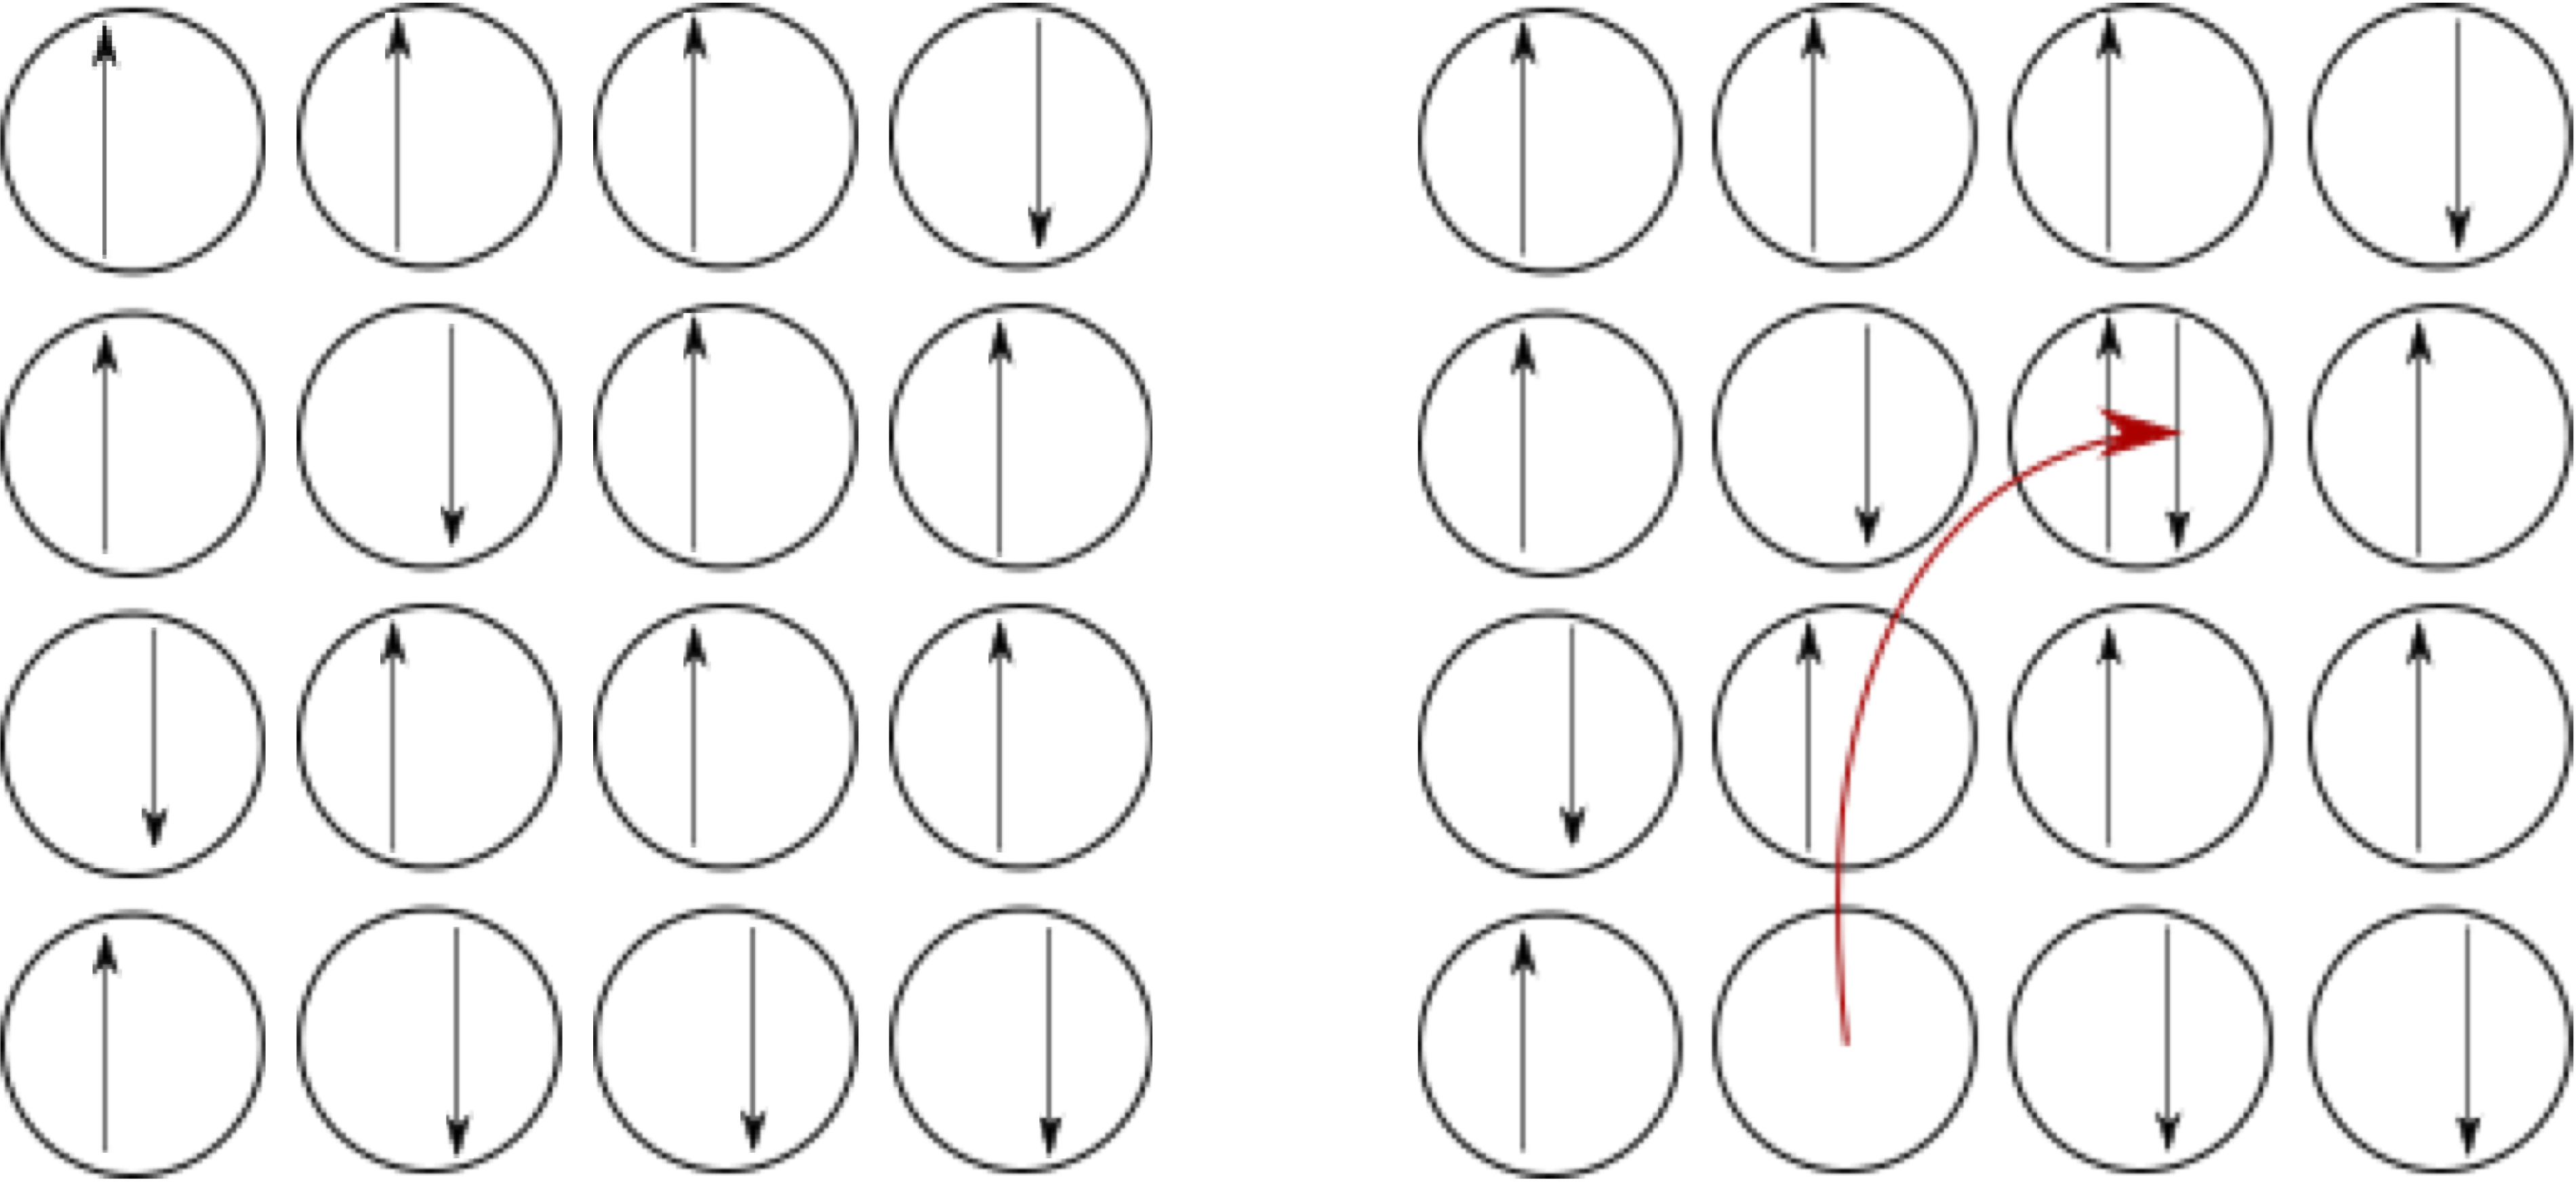
\includegraphics[width = 9cm]{Hubbard/hubbardOneHoleOneDoublyOcV2.png}
\caption[Configuration of the Hubbard model on the square lattice with a hole and a doubly occupied site.]{On the right, a configuration of hydrogen atoms on a square lattice with a hole and a doubly occupied site obtained by delocalization of the spin down electron on the left.}
\end{figure}

If $a$ is large, we have essentially one electron per site at the start.
When an electron is displaced, we end up with a hole and a doubly occupied site.
The potential energy of such a state is
\begin{equation}
E_{H^-} + E_{H^+} - 2 E_H 
\end{equation}

Due to the Coulomb repulsion between the two electrons in $H^-$, this quantity is strictly positive.
Call it $U > 0$.
On the other hand, the system also has kinetic energy: both the hole and the doubly occupied site can delocalize.
Let $W$ be the bandwidth corresponding to the delocalization of an electron on the lattice.
Both the hole and the doubly occupied will stay at the bottom of the band and gain an energy $W/2$ (assuming that this delocalization is of the same order of magnitude).
The dominant transfer integral $-t$ is between nearest neighbors.
The dispersion relation then reads
\begin{equation}
\varepsilon_{\bm k} = -2 t ( \cos k_x + \cos k_y ) 
\end{equation}

The bandwidth is then $W = 8 t$.
The energy of a configuration with a hole and a doubly occupied site is
\begin{equation}
\Delta_c = U - W ,
\end{equation}
where $U$ is practically independent of the lattice parameter $a$.
The bandwidth $W$, however, depends strongly on $a$.
When $a \gg a_0$, where $a_0$ is the Bohr radius, the transfer integral is exponentially small, because only the exponential tails of the wave functions are relevant.
In this limit, $\Delta_c \approx U$ is a large, positive number, and the system is an insulator.
This type of insulator is called a Mott insulator, and $\Delta_c$ is called the charge gap.
As $a$ decreases, $t$ increases, and there must be a critical value $a_c \sim a_0$, for which $U = W$.
Below this value, the computation of $\Delta_c$ is not valid anymore because the gap cannot be negative.
Thus, there must be a metal-insulator transition.
It is possible to see this transition if we apply enough pressure to a Mott insulator so as to decrease $a$ and increase $t$.
A transition of this type was first seen in the 1970's for $V_2 O_3$\footnote{Of course, the transition is not so easy to describe. We should consider the Hubbard model!
However, this simple argument provides an intuitive picture.}.
There is a fundamental difference between a band insulator and a Mott insulator.
While we must pay an energy $\Delta_c$ to make a charge excitation, there is no cost for making a spin excitation: we can flip the spin of an electron without creating a doubly occupied site.
The fluctuations of both charge and spin due to the electron interactions may then lead to magnetic behavior characteristic of correlated  systems.

\section{Computing the partition function for a quadratic Hamiltonian}
\label{sec:Zquadratic}

Let us start by restating the result we want to prove.

If $\mathcal{H} = \bm c^\dagger \bm H \bm c$, where $\bm H$ is a $N \times N$ Hermitian matrix, then we have that
\begin{equation}\label{eq:apZquadratic}
\text{Tr} \big[ e^{-\beta \mathcal{H} } \big] = \prod_{i=1}^N ( 1 + e^{-\beta \lambda_{i} } ) ,
\end{equation}
where $\lambda_{i}$ are the eigenvalues of $\bm H$. 

We will now prove equation (\ref{eq:apZquadratic}). Without loss of generality, let us consider $\bm H$ to be diagonal. Then, its eigenvalues coincide with the diagonal entries, so that $\bm H = \text{diag}(\lambda_{i} )$. The quadratic Hamiltonian may then be diagonalized
\begin{equation*}
\mathcal{H} = {\bm c}^\dagger \text{diag} (\lambda_{1}, \lambda_{2}, .., \lambda_{N}) \bm c = \sum_{i=1}^N \lambda_{i} n_{i}
\end{equation*}

We continue by induction. When $N=1$, we have
\begin{equation}
\text{Tr} (e^{-\beta\mathcal{H} } ) = \left\langle 0 \left| e^{-\beta \lambda_{1} n_{1}}  \right| 0 \right\rangle + \left\langle 1 \left| e^{-\beta \lambda_{1} n_{1}}   \right| 1 \right\rangle = 1 + e^{-\beta \lambda_{1} }
\end{equation}

Assuming that for $N-1$:
\begin{equation*}
\text{Tr} \big[ e^{-\beta \sum_{i=1}^{N-1} \lambda_{i} n_{i} } \big] = \prod_{i=1}^{N-1} ( 1 + e^{-\beta \lambda_{i} } )
\end{equation*}
we can compute the trace for $i$ going up to $N$.
\begin{equation*}
\begin{split}
&\text{Tr} \big[ e^{-\beta \sum_{i=1}^{N-1} \lambda_{i} n_{i} } \big] = \sum_{i=1}^{N} \left\langle \psi_1^{\lambda_1} \psi_2^{\lambda_2} ... \psi_N^{\lambda_N} \left| e^{-\beta \sum_{i=1}^N \lambda_{i} n_{i}}  \right| \psi_1^{\lambda_1} \psi_2^{\lambda_2} ... \psi_N^{\lambda_N} \right\rangle \\
&= \sum_{i=1}^{N-1} \bigg( \left\langle \{\psi_i^{\lambda_i}\} 0 \left| e^{-\beta \sum_{i=1}^N \lambda_{i} n_{i}} e^{-\beta \lambda_{N} n_{N}} \right| \{\psi_i^{\lambda_i}\} 0 \right\rangle + \left\langle \{\psi_i^{\lambda_i}\} 1 \left| e^{-\beta \sum_{i=1}^N \lambda_{i} n_{i}} e^{-\beta \lambda_{N} n_{N}} \right| \{\psi_i^{\lambda_i}\} 1 \right\rangle \bigg) \\
&= (1 + e^{-\beta \lambda_{N} } ) \sum_{i=1}^{N-1} \left\langle \{\psi_i^{\lambda_i}\} \left| e^{-\beta \lambda_{i} n_{i}} \right| \{\psi_i^{\lambda_i}\} \right\rangle \\
&= (1 + e^{-\beta \lambda_{N} } ) \prod_{i=1}^{N-1} (1 + e^{-\beta \lambda_{i} } ) \\
&= \prod_{i=1}^{N} (1 + e^{-\beta \lambda_{i} } )
\end{split}
\end{equation*}

To complete the proof we note that for any $\bm H$, there exists a unitary matrix $\bm Q$, such that $\bm Q^T \bm H \bm Q = \bm \Lambda = \text{diag}(\lambda_{i})$. Let $\tilde{\bm c} = \bm Q \bm c$, and $\tilde{n_i} = \tilde{c_i}^\dagger \tilde{c_i}$. Then, we find
\begin{equation*}
\mathcal{H} = \bm c^\dagger \bm H \bm c = \bm \tilde{\bm c}^\dagger \bm \Lambda \tilde{\bm c} = \sum_{i=1}^N \lambda_{i} \tilde{n}_{i}
\end{equation*}

The trace is independent of the choice of basis functions. Thus, we have
\begin{equation*}
\begin{split}
\text{Tr} ( e^{-\beta \mathcal{H} } ) &= \text{Tr} \bigg( \prod_{i=1}^N e^{-\beta \lambda_{i} \tilde{n}_{i} } \bigg) \\
&= \prod_{i=1}^N \bigg( 1 + e^{-\beta \lambda_{i} } \bigg) \quad\quad \qedsymbol
\end{split}
\end{equation*}

\section{Density of states for a 1D tight binding model}
\label{sec:dos1d}

Using the definition of the density of states
\begin{equation}
N ( E ) = \frac{1}{N} \sum_{\bm k} \delta_{E,\varepsilon_{\bm k}} \rightarrow \frac{1}{(2\pi)^d} \int d\bm k \, \delta ( E - \varepsilon_{\bm k})\,\, \text{when}\,\, N\rightarrow \infty.
\end{equation}
with $\varepsilon_k = - 2 t \cos k$, in the thermodynamic limit we obtain
\begin{equation}
N ( E ) = \frac{1}{2\pi} \int d k \, \delta ( E + 2t \cos k)
\end{equation}

Now we use a well known property of the delta function
\begin{equation}
\delta ( g(x) ) = \sum_{ \{i | g(x_i) = 0\} } \frac{\delta ( x - x_i) }{| g' ( x_i) |}
\end{equation}

Noting that $g'(k) = - 2 t \sin k$, and that the roots of $g$ (there are two in the first Brillouin zone, to which the integral is restricted) satisfy $\cos k_i = - E / 2t$, so that $\sin k_i = \pm \sqrt{1 - E^2 / 4 t^2}$, we obtain
\begin{equation}
\delta ( E + 2 t \cos k) = \frac{1 }{ \sqrt{4t^2 - E^2 }} \bigg( \delta ( k - k_1 ) + \delta ( k - k_2 ) \bigg)
\end{equation}
leading to the sought result
\begin{equation}
N ( E )_{1d} = \frac{1}{\pi \sqrt{4 t^2 - E^2}}
\end{equation}

\section{Effective Heisenberg model as the atomic limit of the Hubbard model}
\label{sec:heisenberg}

To obtain the effective Hamiltonian in the $U/t \gg 1$ limit of the Hubbard model to second order in degenerate perturbation theory, we start with its general form
\begin{equation}
\left \langle m | \mathcal{H}_{\text{eff}} | n \right\rangle = \sum_{ | k \rangle} \frac{\left\langle m | \mathcal{H}_0 | k \right\rangle \left\langle k | \mathcal{H}_0 | n \right\rangle }{E_0 - E_k} =-\frac{1}{U} \sum_{ | k \rangle} \left\langle m | \mathcal{H}_0 | k \right\rangle \left\langle k | \mathcal{H}_0 | n \right\rangle ,
\end{equation}
where $| k \rangle$ are the states that are not in the ground state subspace.
The identity operator in the subspace of states with one doubly occupied site
$
\sum_{ | k \rangle} | k \rangle \langle k |
$
may be written in a more conveniently in the representation:
$
\sum_j n_{j,\sigma} n_{j, -\sigma}
$, 
so that the effective Hamiltonian is
\begin{equation}\label{eq:degPert}
\mathcal{H}_{\text{eff}} = - \mathcal{H}_0 \frac{\sum_j n_{j,\sigma} n_{j, -\sigma}}{U} \mathcal{H}_0
\end{equation}

For each element $j$ of the sum, only terms of the type 
\begin{equation*}
\sum_{i(j)} c_{j,\sigma}^\dagger c_{i,\sigma} 
\end{equation*}
contribute.
Here $\sum_{i(j)}$ is a sum over the set of neighbors $i$ of site $j$.
A term of the effective Hamiltonian $\mathcal{H}_{\text{eff}}$ corresponding to the j-th element in the sum reads
\begin{equation*}
-\frac{t^2}{U} \sum_{i(j), \sigma_1, \sigma_2 } c_{i,\sigma_1}^\dagger c_{j,\sigma_1} n_{j,\sigma} n_{j, -\sigma} c_{j, \sigma_2}^\dagger c_{i, \sigma_2}
\end{equation*}

There are only four cases in which the contribution of a term of this type is nonzero.
\begin{itemize}
\item $\sigma = \sigma_1 = \sigma_2$

The operator in the sum then becomes
\begin{equation*}
c_{i,\sigma}^\dagger c_{j,\sigma} n_{j,\sigma} n_{j, -\sigma} c_{j, \sigma}^\dagger c_{i, \sigma} = n_{i,\sigma} n_{j, -\sigma} c_{j,\sigma} n_{j, \sigma} c_{j, \sigma}^\dagger
\end{equation*}

Now, we use a fermionic operator identity:
\begin{equation*}
\begin{split}
&c n = c c^\dagger c = ( 1 -  c^\dagger c ) c = c \\
&\implies c_{j,\sigma} n_{j,\sigma} c_{j,\sigma}^\dagger = c_{j,\sigma} c_{j,\sigma}^\dagger = 1 - n_{j,\sigma}
\end{split}
\end{equation*}

The term of the Hamiltonian corresponding to this first case then takes on the form
\begin{equation*}
n_{i,\sigma} n_{j,-\sigma} ( 1 - n_{j, \sigma} )
\end{equation*}

We can further simplify this term by noting that in the subspace where $\mathcal{H}_{\text{eff}}$ acts, every site is occupied by only a single electron so that
\begin{equation*}
n_{j,\sigma} + n_{j,-\sigma} = 1 \iff 1 - n_{j,\sigma} = n_{j,-\sigma}
\end{equation*}

Since, for fermions we have that $\hat{n} = \hat{n}^k$, whichever the power $k \in \mathbbm{N}$, the final form of the sought term of the Hamiltonian is
\begin{equation*}
n_{i,\sigma} n_{j, -\sigma}
\end{equation*}

\item $-\sigma = \sigma_1 = \sigma_2$

The contribution to the Hamiltonian is exactly of the same form but making $\sigma \mapsto -\sigma$:
\begin{equation*}
n_{i,-\sigma} n_{j, \sigma}
\end{equation*}

\item $\sigma = - \sigma_1 = \sigma_2$

We can use the same reasoning as we did for the first term to obtain
\begin{equation*}
\begin{split}
&c_{i,-\sigma}^\dagger c_{j,-\sigma} n_{j,\sigma} n_{j, -\sigma} c_{j, \sigma}^\dagger c_{i, \sigma} \\
=& c_{i, -\sigma}^\dagger c_{i,\sigma} \underbrace{c_{j,-\sigma} n_{j, -\sigma}}_{c_{j,-\sigma}} \underbrace{n_{j, \sigma} c_{j, \sigma}^\dagger}_{c_{j,\sigma}^\dagger} \\
=& - c_{i, -\sigma}^\dagger c_{i,\sigma} c_{j, \sigma}^\dagger c_{j,-\sigma}
\end{split}
\end{equation*}

\item $-\sigma = - \sigma_1 = \sigma_2$

Analogously, the contribution to the Hamiltonian is
\begin{equation*}
\begin{split}
&c_{i,\sigma}^\dagger c_{j,\sigma} n_{j,\sigma} n_{j, -\sigma} c_{j, -\sigma}^\dagger c_{i, -\sigma} \\
=& - c_{i, -\sigma}^\dagger c_{i,\sigma} c_{j, \sigma}^\dagger c_{j,-\sigma}
\end{split}
\end{equation*}

\end{itemize}

Grouping all these four terms, we obtain
\begin{equation}
\mathcal{H}_{\text{eff}} = \frac{2t^2}{U} \sum_{\left\langle i, j \right\rangle, \sigma} ( - n_{i,\sigma} n_{j,-\sigma} + c_{i,-\sigma}^\dagger c_{i,\sigma} c_{j,\sigma}^\dagger c_{j,-\sigma} ) ,
\end{equation}
where the factor of 2 appears because for each pair of nearest neighbors $\left\langle i, j \right\rangle$, a term comes from the term $n_{j,\sigma} n_{j,-\sigma}$ of the sum $\sum_j n_{j,\sigma} n_{j,-\sigma}$, and another term from $n_{i,\sigma} n_{i,-\sigma}$.

Recall the second quantized form of the spin operators:
\begin{equation}
\begin{cases}
S_i^z = \frac{1}{2} ( n_{i,\uparrow} - n_{i,\downarrow} ) \\
S_i^+ = c_{i,\uparrow}^\dagger c_{i,\downarrow} \\
S_i^- = c_{i,\downarrow}^\dagger c_{i,\uparrow}, \\
\end{cases}
\end{equation}

Using these relations and that the density operator is $n_i = n_{i,\uparrow} + n_{i,\downarrow}$, the following relations hold
\begin{equation}
\begin{split}
S_i^z S_j^z - \frac{1}{4} n_i n_j &= -\frac{1}{2} ( n_{i,\uparrow} n_{j,\downarrow} + n_{i,\downarrow} n_{j,\uparrow} ) \\
S_i^+ S_j^- + S_i^- S_j^+ &= c_{i,\uparrow}^\dagger c_{i,\downarrow} c_{j,\downarrow}^\dagger  c_{j,\uparrow} +  c_{i,\downarrow}^\dagger c_{i,\uparrow} c_{j,\uparrow}^\dagger  c_{j,\downarrow}
\end{split}
\end{equation}

Thus, we may rewrite the effective Hamiltonian:
\begin{equation}
\mathcal{H}_{\text{eff}} = \frac{4t^2}{U} \sum_{\left\langle i, j \right\rangle} \bigg( S_i^z S_j^z - \frac{1}{4} n_i n_j + \frac{1}{2} ( S_i^+ S_j^- + S_i^- S_j^+ ) \bigg)
\end{equation}

But $S_i^z S_j^z + \frac{1}{2} ( S_i^+ S_j^- + S_i^- S_j^+) = \bm S_i \cdot \bm S_j$ and $n_i = n_j = 1$ in the ground state subspace, so the effective Hamiltonian becomes
\begin{equation}
\mathcal{H}_{\text{eff}} = \frac{4t^2}{U} \sum_{\left\langle i, j \right\rangle} \bigg( \bm S_i \cdot \bm S_j  - \frac{1}{4}  \bigg),
\end{equation}
which corresponds to the antiferromagnetic Heisenberg model: $\mathcal{H}_{\text{Heis}} = J \sum_{\left\langle i, j \right\rangle} \bm S_i \cdot \bm S_j $, with $J = 4 t^2 / U$.

\section{On Wick's theorem}
\label{sec:wick}

A product of operators containing $k$ factors $c_i^\dagger$ and $n - k$ factors $c_i$ is brought into \emph{normal ordering} by the operator $\mathcal{N}$ (also written $: \,\,:$) defined as
\begin{equation}
\mathcal{N} [ c_1^{(\dagger)} c_2^{(\dagger)} ... c_n^{(\dagger)} ] = :  c_1^{(\dagger)} c_2^{(\dagger)} ... c_n^{(\dagger)}  : \, \equiv ( - 1 )^P c_{i_1}^{\dagger} c_{i_2}^{\dagger} ... c_{i_k}^{\dagger} c_{i_{k+1}} ... c_{i_n} ,
\end{equation}
where $P$ is the parity of the permutation $1, 2, ..., n \mapsto i_1, i_2, ..., i_n$.

It is straightforward to simplify a product of two operators: $C_1 C_2 = \mathcal{N} [ C_1 C_2 ] + \{ C_1^- , C_2^+ \} $, using the anti-commutation rules.
Here $C_i^{\Pm}$ is a combination of fermionic creation (annihilation) operators. 
The last term is a c-number by assumption.
Defining a contraction as $\contraction{}{C}{ {}_1 }{C_2}
C_1 C_2 \equiv C_1 C_2 - \mathcal{N}[ C_1 C_2 ]$, we obtain $\contraction{}{C}{ {}_1 }{C_2}
C_1 C_2 =  \{ C_1^- , C_2^+ \}  $.
The definition of a contraction holds even there are other operators between the two contracted ones $C_{1, 2}$.
Wick's theorem generalizes the resullt for a product of two operators, giving an expression for the product of an arbitrary number of operators.

Let us state the zero temperature version of Wick's theorem for generic operators $C_i= C_i^+ + C_i^-$.
\begin{equation}\label{eq:wickState}
C_1 C_2 ... C_n = \mathcal{N} [ C_1 C_2 ... C_n ] + \sum_{(ij)} \mathcal{N} [ C_1 C_2 ...
\contraction{}{C_i}{...}{C_j}
C_i ... C_j ... C_n ]
+ \sum_{(ij), (lm)} \mathcal{N} [ C_1 C_2 ...
\contraction{}{C}{ {}_i ... C_l ... }{C_j}
C_i ... 
\contraction[2ex]{}{C}{ {}_l ... C_j ... }{C_m}C_l ... C_j ... C_m ... C_n ] + ... ,
\end{equation}
where the first sum is over single contractions of pairs, the second one on double contractions, and so on.
For odd $n$, the last term contains single unpaired operators.
Otherwise, they are just products of contractions, which are c-numbers.

A general rule follows from the fact that the average of a normally ordered operator vanishes in the ground state.
Two-point correlation functions determine all $n$-point correlation functions.
In particular, for the case of 4 operators, using a self-explanatory abbreviated notation:
\begin{equation}
\left\langle gs | 1234 | gs \right\rangle = \left\langle 12 \right\rangle \left\langle 34 \right\rangle - \left\langle 13 \right\rangle \left\langle 24 \right\rangle + \left\langle 14 \right\rangle \left\langle 23 \right\rangle
\end{equation}

Of course, in the finite temperature case, Wick's theorem is not an operator identity because there is no non ambiguous way of defining normal ordering.
However, for non-interacting particles, the thermal average of a product of one-particle operators is still a sum over all possible contractions of pairs.
All that changes is the definition of the contraction, which is now defined in terms of the thermal average of the product of a pair of operators.
Additionally, the theorem generalizes for time-ordered products, simply by replacing the thermal averages of the pair products by time-ordered pair averages.

In particular, for a free theory, the $n$-particle Green's function, defined by the field operators $\hat{\psi} ( x )$,
\begin{equation}
\mathcal{G} ( x_1, x_2, ..., x_n; y_1, y_2, ... y_n ) \equiv \left\langle \mathcal{T} \hat{\psi} ( x_1 ) \hat{\psi} ( x_2 ) ... \hat{\psi} ( x_n ) \hat{\psi}^\dagger ( y_1 ) \hat{\psi}^\dagger ( y_2 ) ... \hat{\psi}^\dagger ( y_n ) \right\rangle
\end{equation}
is determined solely by the set of all one-particle Green's functions.
Here $x$ and $y$ denote both the complete set of quantum numbers describing the system's degrees of freedom, and imaginary time.

Applying Wick's theorem to the set of non-interacting (and thus independent) particles, we obtain
\begin{equation}
\mathcal{G} ( x_1, x_2, ... x_n; y_1, y_2,... y_n ) = \sum_P (- 1 )^P \mathcal{G}^0 ( x_1; y_{i_1} ) \mathcal{G}^0 ( x_2; y_{i_2} ) ... \mathcal{G}^0 ( x_n; y_{i_n} ) ,
\end{equation}
which corresponds to evaluating the determinant of the matrix $\bm G$, defined as $G_{ij} \equiv \mathcal{G}^0 ( x_i ; x_j )$ for $i, j = 1, 2, ..., n$, where the $\mathcal{G}^0$ are the free-particle Green's functions, also called propagators.

\section{Mean field theory and the variational principle}
\label{sec:mftVariational}

In section \ref{sec:hartree-fock}, we derived the Hartree-Fock form of the Hubbard Hamiltonian.
Here we explain how it arises as a mean field theory prone to studying spontaneous symmetry breaking, generally by resorting to a self-consistent procedure.
This is useful as a first approach to investigate the tendency towards long range ordering, for example in ferromagnetic, or antiferromagnetic phases.

The starting point is the Gibbs-Bogoliubov-Feynman (GBF) inequality
\begin{equation}\label{eq:gibbs}
\mathcal{F} \le \left\langle \mathcal{H} \right\rangle_{\text{MF}} - T \mathcal{S}_{\text{MF}} ,
\end{equation}
which is saturated when $\mathcal{H}_{\text{MF}} = \mathcal{H}$, and in general  serves as a variational principle to find a simpler, non-interacting form for the Hamiltonian.
$\mathcal{F}$ is the system's free energy, $T$ is the temperature and the mean field averages are computed as per Eq.(\ref{eq:mfAv}), while the entropy is computed for the thermal distribution $\rho_{\text{MF}} = e^{-\beta \mathcal{H}_{\text{MF}}}$.
Defining $\mathcal{F}_{\text{MF}} = \left\langle \mathcal{H}_{\text{MF}} \right\rangle_{\text{MF}} - T \mathcal{S}_{\text{MF}}$, we may recast Eq.(\ref{eq:gibbs}) as
\begin{equation}\label{eq:gibbs2}
\mathcal{F} \le \mathcal{F}_{\text{MF}} + \left\langle \mathcal{H} - \mathcal{H}_{\text{MF}} \right\rangle_{\text{MF}} \equiv F
\end{equation}

We seek a quadratic Hamiltonian that minimizes $F$, i.e. $\delta F = 0$, of the form
\begin{equation}\label{eq:hMF}
\mathcal{H}_{\text{MF}} = \mathcal{H}_K + \sum_{i, j, \sigma} \varepsilon_{ij} c_{i, \sigma}^\dagger c_{j, \sigma} ,
\end{equation}
which corresponds to the possibility of the  appearance of spin polarization along the quantization axis.
and by varying $\varepsilon_{ij} \mapsto \varepsilon_{ij} + \delta \varepsilon_{ij} $, we can compute $\delta F$ and show that it is minimized ($\delta F = 0$) for the mean field Hubbard Hamiltonian in much the same way as we did in section \ref{sec:hartree-fock}.

Since the Hamiltonian of Eq.(\ref{eq:hMF}) is quadratic in the fermion operators, we have that $ \left\langle n_{i,\uparrow} n_{i,\downarrow} \right\rangle_{\text{MF}} = \left\langle n_{i,\uparrow} \right\rangle_{\text{MF}} \left\langle n_{i,\downarrow} \right\rangle_{\text{MF}}$, and we must vary $\varepsilon_{ij}$ in the following term
\begin{equation}
\left\langle \mathcal{H} - \mathcal{H}_{\text{MF}} \right\rangle_{\text{MF}} = \sum_{i, j, \sigma} \bigg( \frac{U}{2} \left\langle n_{i,\sigma} \right\rangle_{\text{MF}} \left\langle n_{j,-\sigma} \right\rangle_{\text{MF}} \delta_{ij} -\varepsilon_{ij} \left\langle c_{i,\sigma}^\dagger c_{j, \sigma} \right\rangle_{\text{MF}} \bigg),
\end{equation}
leading to
\begin{equation}
\delta \left\langle \mathcal{H} - \mathcal{H}_{\text{MF}} \right\rangle_{\text{MF}} = \sum_{i, j, \sigma} \bigg( U \left\langle n_{i,\sigma} \right\rangle_{\text{MF}} \delta \left\langle n_{j,-\sigma} \right\rangle_{\text{MF}} \delta_{ij} - \delta \varepsilon_{ij} \left\langle c_{i,\sigma}^\dagger c_{j, \sigma} \right\rangle_{\text{MF}} - \varepsilon_{ij} \delta \left\langle c_{i,\sigma}^\dagger c_{j, \sigma} \right\rangle_{\text{MF}} \bigg)
\end{equation}

The mean field free energy term can be obtained by introducing the variation $\mathcal{H} \mapsto \mathcal{H} + \delta \mathcal{H} $.
\begin{equation}\label{eq:varTr}
\begin{split}
\Tr [ e^{-\beta ( \mathcal{H} + \delta \mathcal{H} ) } ] &= \Tr  \bigg[ \sum_n \frac{(-\beta)^n}{n!} ( \mathcal{H} + \delta \mathcal{H} )^n \bigg] \\
&= 1 + \Tr \bigg[  \sum_{n=1}^{\infty} \frac{(-\beta)^n}{n!} \mathcal{H}^n \bigg] \\
& + \Tr \bigg[  \sum_{n=1}^{\infty} \frac{(-\beta)^n}{n!} (\delta \mathcal{H} \mathcal{H}^{n-1} +  \mathcal{H} \delta \mathcal{H} \mathcal{H}^{n-2} + \mathcal{H}^2 \delta \mathcal{H} \mathcal{H}^{n-3} + ... \mathcal{H}^{n-1} \delta \mathcal{H} ) \bigg] + \mathcal{O} ( \delta \mathcal{H}^2 ) \\
&= \Tr [ e^{-\beta \mathcal{H} } ] + \Tr \bigg[ \delta \mathcal{H} \sum_{n=1}^\infty \frac{(-\beta)^n}{(n-1)!} \mathcal{H}^{n-1} \bigg] + \mathcal{O} ( \delta \mathcal{H}^2 ) \\
&= \Tr [ e^{-\beta \mathcal{H} } ] - \beta \Tr \bigg[ \delta \mathcal{H} e^{-\beta \mathcal{H} } \bigg] + \mathcal{O} ( \delta \mathcal{H}^2 )
\end{split} ,
\end{equation}
which, in turn, implies that
\begin{equation}\label{eq:dTr}
\delta \Tr [ e^{-\beta \mathcal{H} } ] = -\beta \Tr [ e^{-\beta \mathcal{H} } \delta \mathcal{H} ] 
\end{equation}
and, using the definition of the mean field free energy:
\begin{equation}\label{eq:fMF}
\delta \mathcal{F}_{\text{MF}} = -\frac{1}{\beta} \delta \bigg( \ln ( \Tr [ e^{-\beta \mathcal{H}_{\text{MF}} } ] ) \bigg) = -\frac{1}{\beta} \frac{\delta \big( \Tr [e^{-\beta \mathcal{H}_\text{MF}} ] \big) }{\Tr [e^{-\beta \mathcal{H}_\text{MF}} ]} ,
\end{equation}
and replacing Eq.(\ref{eq:dTr}) in Eq.(\ref{eq:fMF}), we may gather all the terms to finally arrive at
\begin{equation}
\begin{split}
\delta F &= \delta \mathcal{F}_{\text{MF}} + \delta \left\langle \mathcal{H} - \mathcal{H}_{\text{MF}} \right\rangle_{\text{MF}} \\
&= \sum_{i, j, \sigma} \bigg( U \left\langle n_{i,-\sigma} \right\rangle_{\text{MF}} \delta \left\langle n_{j,\sigma} \right\rangle_{\text{MF}} \delta_{ij} - \varepsilon_{i j} \delta \left\langle c_{i, \sigma}^\dagger c_{j, \sigma} \right\rangle_{\text{MF}} \bigg) \\
&= \sum_{i, j, \sigma} \bigg( U \left\langle n_{i,-\sigma} \right\rangle_{\text{MF}} \delta \left\langle c_{i, \sigma}^\dagger c_{j,\sigma} \right\rangle_{\text{MF}} \delta_{ij} - \varepsilon_{i j} \delta \left\langle c_{i, \sigma}^\dagger c_{j, \sigma} \right\rangle_{\text{MF}} \bigg) = 0 \\
&\implies \varepsilon_{i j} = U \left\langle n_{i,-\sigma} \right\rangle_{\text{MF}} \delta_{i j} 
\end{split}
\end{equation}
leading to the mean field approximation for the Hubbard model:
\begin{equation}
\mathcal{H}_{\text{MF}} = \mathcal{H}_K + U \sum_{i, \sigma} \left\langle n_{i,- \sigma} \right\rangle_{\text{MF}} n_{i, \sigma}
\end{equation}

Although the mean field equations can be obtained both from $\delta \mathcal{F}_{\text{MF}} = 0$ and from $\delta F = 0$, this only means that they both have a vanishing functional derivative at a given (common) configuration of the system.
There may be other configurations at which $\delta \mathcal{F}_{\text{MF}}$ vanishes, but we have only an extremum.
Thus, we must be cautious when analyzing self-consistent solutions to confirm that they indeed correspond to a minimum of the functional $F$, and not only an extremum of $\mathcal{F}_{\text{MF}}$.

On a final note, we remark that this procedure can be generalized to the \ac{GCE} by considering the GBF inequality for the grand potential $\Omega_G$:
\begin{equation}\label{eq:gibbsGrand}
\Omega_G \le \Omega_{\text{MF}} + \left\langle \mathcal{H} - \mathcal{H}_{\text{MF}} \right\rangle_{\text{MF}} \equiv \Omega ,
\end{equation}
where we defined $\Omega_{\text{MF}} = \left\langle \mathcal{H}_{\text{MF}} \right\rangle_{\text{MF}} - T \mathcal{S}_{\text{MF}}- \mu \left\langle \mathcal{N} \right\rangle_{\text{MF}}$, $\mathcal{N}$ being the total number operator.
The iterative scheme we use to solve the self consistent equation is not a minimization algorithm.
However, if it does not get stuck in a metastable state, it tends to take steps towards minimizing the functional $\Omega$.
This is illustrated in Fig.(\ref{fig:grandPotMin}).
The data was obtained by solving the self consistent equation for the generalized intra-orbital version of the Hubbard model we use throughout.
The model is obtained from the 3-band tight binding Hamiltonian of the first chapter, and by adding an on-site and intra-orbital interaction.
In this case, we consider a \acs{TMD} nanoribbon with $N_y = 16$, at inverse temperature $\beta t = 2 $, at $U = 16$, where $U$ is an on-site interaction that only occurs if the electrons occupy the same $d$-orbital.
Thus, only double occupancy of a site \emph{and an orbital} is penalized.

\begin{figure}[H]
\centering
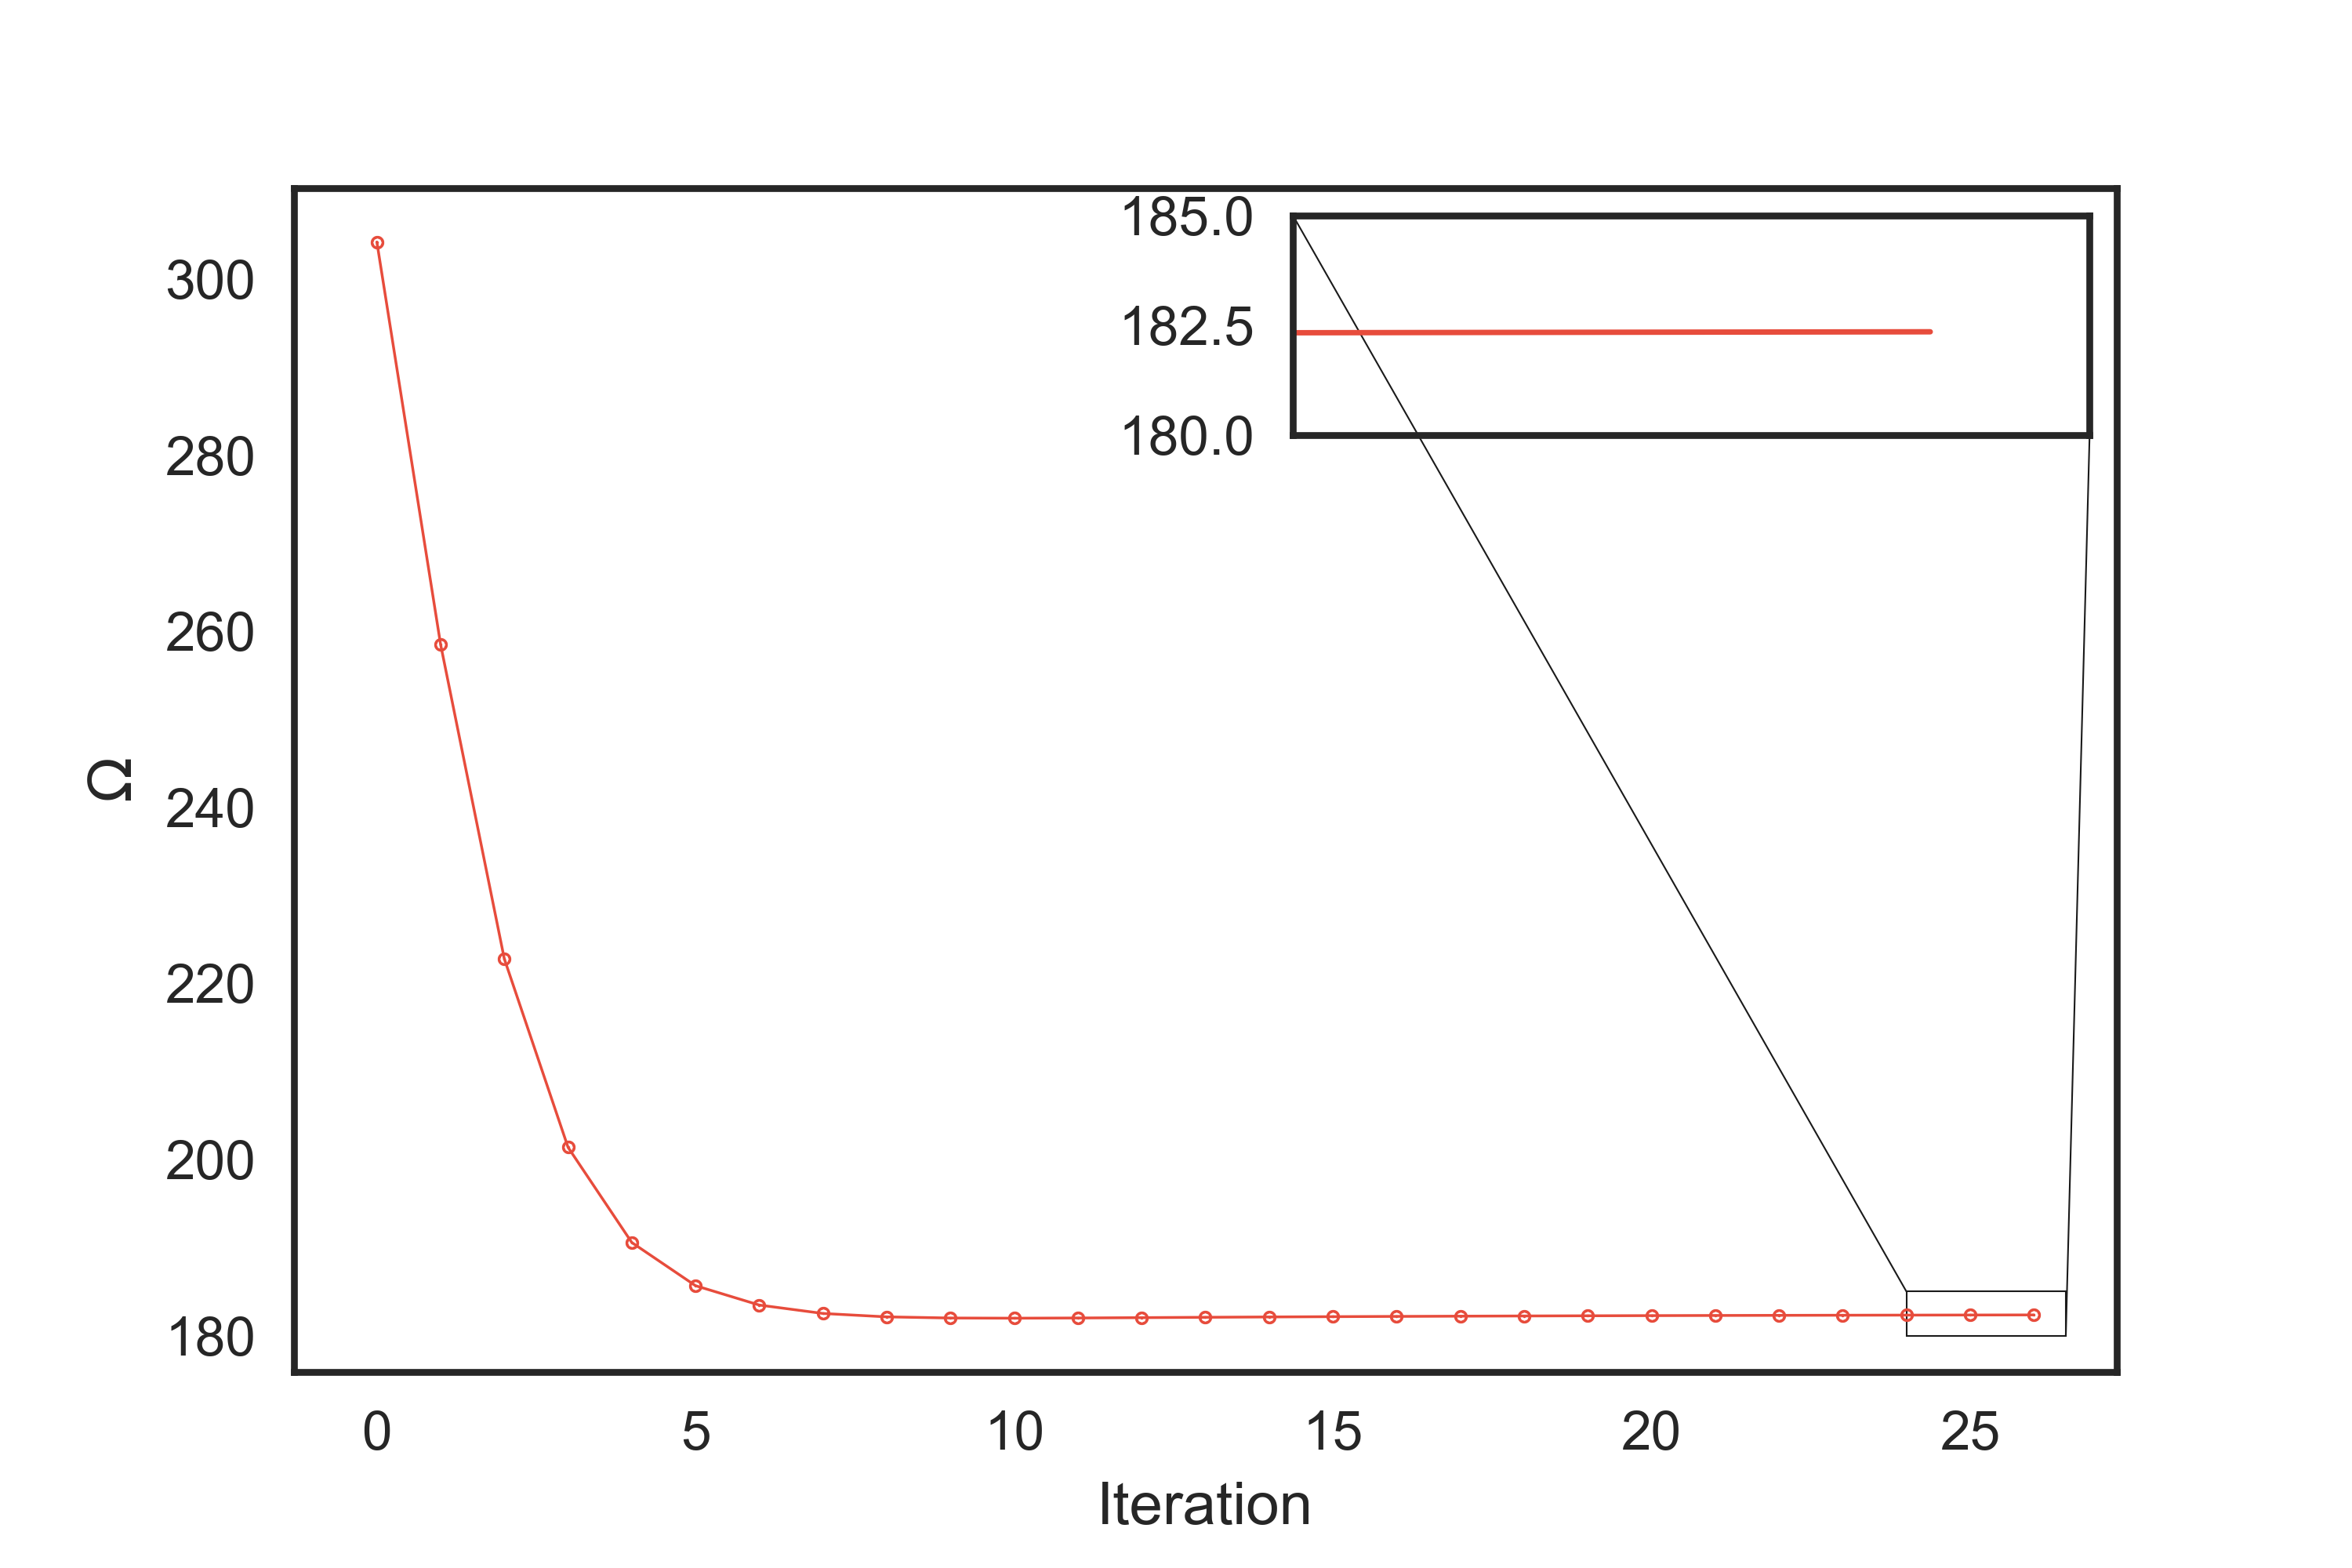
\includegraphics[scale=0.55]{Applications/grandpotMin_Nx=512_Ny=16_U=16_beta=2.png}
	\caption[Example of the minimization of the grandpotential functional.]{Example of the minimization of the grandpotential functional $\Omega$ for a TMD nanoribbon of width $N_y = 16$, at inverse temperature $\beta = 2 t $, at $U = 16$. \label{fig:grandPotMin}}
\end{figure}   
		\chapter{On the finite temperature Wick's theorem}
\label{ap:wick}

\pagebreak

\begin{equation}
\contraction{}{A}{B}{C}
\contraction[2ex]{A}{B}{C}{D}
ABCD
\end{equation}



$$
\contraction{}{A}{...}{B}
%
A...B
$$
		\cleardoublepage
	\end{appendix}
\end{appendices}


\end{document}